\documentclass[12pt]{article}
%!TEX root = ../notas_de_clase.tex

%preamble

 
\usepackage[letterpaper, portrait, margin=0.8in]{geometry}
%language
\usepackage[spanish,es-nodecimaldot]{babel}
\usepackage[utf8]{inputenc}
\usepackage{apacite}



%packages
\usepackage[Algoritmo]{algorithm}
\usepackage{algorithmicx}
\usepackage[noend]{algpseudocode}
\usepackage{mathtools}
\setlength {\marginparwidth }{2cm}
\usepackage{todonotes}
\usepackage{amsbsy}
\usepackage{amssymb}
\usepackage{amsmath,bm}

\usepackage{xcolor}
\providecommand{\red}[1]{\textcolor{red}{#1}}
\usepackage{graphicx}
\usepackage{fancybox}
\usepackage{booktabs}
\usepackage{caption}
\usepackage{float}
%\usepackage[longend,ruled,algochapter,linesnumbered,lined,boxed,commentsnumbered,spanish]{algorithm2e}
%\usepackage[algo2e]{algorithm2e}
\usepackage{amssymb}
\usepackage{amstext}
\usepackage{bm}
\usepackage{wrapfig}
\usepackage{subcaption} % para_unsupervised_chapter

%formatting


\ifx\byn\undefined
    \definecolor{my_blue}{HTML}{C2D5FF}
    \definecolor{my_red}{HTML}{FFC2C2}
\else
    \definecolor{my_blue}{HTML}{FFFFFF}
    \definecolor{my_red}{HTML}{FFFFFF}
\fi


\usepackage[framemethod=TikZ]{mdframed}
\mdfdefinestyle{discusion}{%
    %linecolor=black,
    %outerlinewidth=0pt,
    roundcorner=0pt,
    innertopmargin=\baselineskip,
    innerbottommargin=\baselineskip,
    innerrightmargin=20pt,
    innerleftmargin=20pt,
    backgroundcolor=my_blue}
    
\colorlet{Green}{green!90}

\mdfdefinestyle{pendiente}{%
    style = discusion, 
    backgroundcolor=my_red}


\RequirePackage{url}

%definitions
\def\td{{\text d}}
\def\R{{\mathbb R}}
\def\cN{{\mathcal N}}
\def\N{{\mathbb N}}
\def\datos{{\mathcal T}}
\def\eye{{\mathbb I}}
\def\ssum{{\scriptstyle\sum}}
\def\bepsilon{{\bm \epsilon}}
\def\tx{\tilde{x}}
\def\tX{\tilde{X}}
\newcommand{\gp}{\ensuremath{\mathcal{GP}}}
\newcommand{\pr}{\ensuremath{\mathbb{P}}}
\newcommand{\x}{\ensuremath{\mathbf{x}}}
\newcommand{\z}{\ensuremath{\mathbf{z}}}
\newcommand{\cvector}{\ensuremath{\mathbf{c}}}
\newcommand{\e}{\ensuremath{\mathbf{e}}}
\newcommand{\y}{\ensuremath{\mathbf{y}}}
\newcommand{\bx}{\ensuremath{\textcolor{blue}{X}}}
\newcommand{\by}{\ensuremath{\textcolor{blue}{Y}}}
\newcommand{\rx}{\ensuremath{\textcolor{red}{X_*}}}


\DeclareMathOperator*{\argmax}{arg\,max}
\DeclareMathOperator*{\argmin}{arg\,min}
\DeclareMathOperator{\E}{\mathbb{E}}
\DeclareMathOperator{\V}{\mathbb{V}}
\newcommand\deq{\stackrel{\mathclap{\normalfont\mbox{\tiny def}}}{=}}
%\newcommand{\E}[1]{\mathbb E \left[#1\right]}



%\newcommand{\R}{\mathbb{R}}
\author{{ Felipe Tobar}\\Universidad de Chile}
\title{\vspace{7cm} Aprendizaje de Máquinas}
%!TEX root = notas_de_clase.tex

% --------------------------------------------------------------------
% Definitions (do not change this)
% --------------------------------------------------------------------
\newcommand{\HRule}[1]{\rule{\linewidth}{#1}} 	% Horizontal rule

\makeatletter							% Title
\def\printtitle{%						
    {\centering \@title\par}}
\makeatother									

\makeatletter							% Author
\def\printauthor{%					
    {\centering \large \@author}}				
\makeatother							

% --------------------------------------------------------------------
% Metadata (Change this)
% --------------------------------------------------------------------
\title{	\normalsize \textsc{Notas de clase} 	% Subtitle
		 	\\[6.0cm]								% 2cm spacing
			\HRule{0.5pt} \\						% Upper rule
			 \textbf{\uppercase{\LARGE Aprendizaje de Máquinas}}	% Title
			\HRule{2pt} \\ [0.5cm]		% Lower rule + 0.5cm spacing
			\large Versión: \today			% Todays date
		}

\author{
		Felipe Tobar\\	
		Centro de Modelamiento Matemático\\	
		Universidad de Chile\\
        \texttt{ftobar@dim.uchile.cl} \\[1.0cm]
}

\begin{document}
% Maketitle
\thispagestyle{empty}		% Remove page numbering on this page
\printtitle					% Print the title data as defined above
  	\vfill
\printauthor				% Print the author data as defined above
\newpage
% 

%!TEX root = notas_de_clase.tex
\newpage
\section*{Prefacio}
Este apunte es una versión extendida de las notas de clase del curso \emph{MA5203: Aprendizaje de Máquinas Probabilístico} dictado en el Departamento de Ingeniería Matemática, Universidad de Chile. En este sentido, este apunte contiene estrictamente más contenidos que los vistos en clases en cada una de las unidades que componen el curso. 

El fin último de este apunte es ser un libro autocontendio y original de las temáticas vistas en el curso arriba mencionado. Sin embargo, un objetivo importante es también apoyar el desarrollo del curso para que los alumnos puedan avanzar en los contenidos de éste de forma independiente en base a una fuente unificada. Por esta razón, esta versión preliminar del apunte está disponible para los alumnos del curso, en donde hay aún inconsistencias de formato, figuras o completitud de contenidos. En este sentido, este apunte será continuamnete actualizado. 

Este esfuerzo ha sido posible gracias a la contribución de varios integrantes del cuerpo académico del curso MA5203 durante los años 2016, 2017 y 2018. Me gustaría reconocer la indispensable contribución de ayudantes del curso durante estos años, tanto en el desarrollo del curso mismo como en la escritura de secciones del apunte: Alejandro Cuevas, Gonzalo Ríos, Alejandro Veragua, Nicolás Aramayo, Lerko Araya, Mauricio Campos, Cristóbal Silva y Cristóbal Valenzuela. Sin la participación de todos ellos el éxito del curso y la composición de este apunte no habrían sido posible.


\bigskip
\begin{flushright}
  Felipe Tobar\par
  \today\par
  Santiago, Chile
\end{flushright}
\newpage


\tableofcontents
\newpage
%!TEX root = ../notas_de_clase.tex


\section{Introducción}


El aprendizaje de máquinas (AM) es una disciplina que reúne elementos de ciencias de la computación, optimización, estadística, probabilidades y ciencias cognitivas para construir el motor de aprendizaje dentro de la Inteligencia Artificial. Definido por Arthur Samuel en 1950, el AM es la disciplina que da a las máquinas la habilidad de aprender sin ser explícitamente programadas. Si bien existen enfoques al AM inspirados en sistemas biológicos, esta no es la única forma de construir métodos de aprendizaje: una analogía se puede identificar en los primeros intentos por construir máquinas voladoras, en donde se pretendía replicar el movimiento de las alas de un pájaro, sin embargo, estos intentos no fueron exitosos y no fue sino hasta la invención del primer avión, el cual no mueve sus alas, que el hombre logró construir la primera máquina voladora. Esto sugiere que el paradigma biológico no es exclusivo al momento de construir máquinas inteligentes que utilicen observaciones de su entorno para extraer información útil y generar predicciones. 


AM es una disciplina joven que ha experimentado un vertiginoso crecimiento en las últimas décadas, esto ha sido posible en gran parte gracias a los recientes avances computacionales y la cantidad de datos que permite entrenar modelos complejos. El uso masivo de técnicas AM se ha visto reflejado en distintas áreas que incluyen visión computacional, clasificación de secuencias de ADN, marketing, detección de fraude, diagnósticos médicos, análisis financiero y traducción de texto por nombrar algunas. Adicionalmente, si bien el objetivo de AM es desarrollar algoritmos de aprendizaje prescindiendo en gran medida de la intervención humana,  otra razón del éxito del AM es su facilidad para acoplarse con otras disciplinas aplicadas, en particular al área que hoy conocemos como \textit{Data Science}. 

\subsection{Orígenes: Inteligencia Artificial}

Nuestras habilidades cognitivas nos diferencian fuertemente del resto de las especies del reino animal y el dominio del \emph{Homo sapiens} sobre el planeta radica en estas habilidades: la inteligencia humana superior a la del resto de los animales nos permite adaptarnos a diferentes situaciones ambientales y sociológicas de forma rápida y sin la necesidad de un cambio evolutivo. Por ejemplo, para migrar desde África al norte de Europa y a Oceanía, el \emph{Homo sapiens} no se adaptó biológicamente a climas distintos, sino que manipuló herramientas y materiales para producir vestimenta adecuada y embarcaciones. Otra característica única del \emph{Homo sapiens} es su habilidad de creer en un imaginario colectivo que permite construir organizaciones con un gran número de individuos, lo cual nuevamente exclusiva a nuestra especie y consecuencia de nuestra inteligencia \cite{harari}. 

Nuestro interés en entender la inteligencia puede ser identificado desde los comienzos de la Filosofía y Sicología, disciplinas que se han dedicado al estudio de las forma en que entendemos, recordamos, razonamos y aprendemos. La inteligencia artificial (IA) es una disciplina mucho más reciente que las anteriores y va un paso más allá de la mera comprensión de la inteligencia, pues apunta a replicarla e incluso mejorarla \cite{bostrom_2014}. Hay varias definiciones de IA dependiendo de si (i) adoptamos un punto de vista de razonamiento versus comportamiento, o bien si (ii) identificamos las acciones inteligentes como humanas u objetivamente racionales, una de estas posiciones es la de Alan Turing, el que mediante el juego de la imitación \cite{turing_1950}, sentencia que una máquina es inteligente si es capaz de desarrollar tareas cognitivas a un nivel “humano” suficiente para engañar a un interrogador (también humano). En este contexto para que una máquina sea inteligente, o equivalentemente, apruebe el test de Turing, es necesario que posea \cite{russell_norvig_2009}:  
\begin{itemize}
	\item \textbf{procesamiento de lenguaje natural} para comunicarse con seres humanos, en particular, el interrogador,
	\item \textbf{representación del conocimiento} para guardar información recibida antes y durante la interrogación,
	\item \textbf{razonamiento automático} para usar la información guardada y formular respuestas y conclusiones, y
	\item \textbf{aprendizaje de máquinas} para adaptarse a nuevas circunstancias y descubrir patrones.
\end{itemize}

El test de Turing sigue siendo un tópico de investigación en Filosofía hasta el día de hoy, sin embargo, los avances actuales de la inteligencia artificial no están necesariamente enfocados en diseñar máquinas para aprobar dicho test. Si bien los inicios de la IA están en la Filosofía, actualmente los avances en IA apuntan a desarrollar metodologías para aprender de grandes volúmenes de información sin necesariamente actuar de forma humana, en particular, el componente de aprendizaje de máquinas en la lista anterior ha jugado un papel fundamental en esta nueva etapa, en donde su aporte en distintas áreas de aplicación es cada vez más evidente. 


\subsection{Breve historia del aprendizaje de máquinas}

En base a las definiciones de la inteligencia de máquinas asentadas por Turing en 1950, las primeras redes neuronales artificiales comenzaron a emerger en los trabajos seminales de (Minsky, 1952) que programó el primer simulador de una red neuronal,  (Farley \& Clark, 1954) que implementaron un algoritmo de prueba y error para el aprendizaje, y (Rosenblatt, 1958) que propuso el Perceptrón. En los años siguientes la investigación en redes neuronales se vio afectada por las limitaciones de dichas estructuras expuestas en (Minsky \& Papert, 1969) dando origen a lo que es conocido como el primer invierno de la inteligencia artificial, en donde el Profesor Sir James Lighthill expuso frente al parlamento inglés que la inteligencia artificial se fijaba objetivos no realistas y solo servía para escenarios básicos (Lighthill, 1973). Esta desconfianza en los alcances de la IA ralentizó su desarrollo, sin embargo, los conexionistas  seguirían investigando sobre formas de diseñar y entrenar redes neuronales, específicamente, los resultados de (Werbos, 1974) que culminarían en el algoritmo de backpropagation propuesto por (Rumelhart, Hinton, \& Williams, 1986) y los avances de  (Hopfield, 1982) en redes neuronales recurrentes permitirían terminar con el primer invierno de la inteligencia artificial.  
 
Durante el receso del conexionismo proliferaron los sistemas basados en reglas, en particular, los sistemas experto compuestos por una serie de reglas condicionales “si-entonces” (if-then) que replican el comportamiento de un humano experto, estos métodos se convirtieron en la primera herramienta exitosa de la IA en aplicaciones reales. Sin embargo, los sistemas experto no aprenden por sí solos, en el sentido de que las reglas si-entonces deben ser explícitamente programadas por un humano, esto tiene un costo considerable dependiendo de la complejidad del problema, por lo que hacia el comienzo de la década de los 90s los sistemas experto colapsaron debido a que la cantidad de información disponible aumentaba y dicho enfoque no es “escalable”. Un sistema basado en regla que aún se utiliza son los llamado árboles de decisión (Breiman, Friedman, Olshen, \& Stone, 1984), los cuales difieren de los sistemas experto en que las reglas no son definidas por un humano sino que descubiertas en base a la elección de variables que mejor segmentan los datos de forma supervisada.

Las redes neuronales vieron un resurgimiento en los 80s con el método de backpropagation que permitía entrenar redes neuronales de más de dos capas usando la regla de la cadena, esto permitió finalmente validar la premisa conexionista en tareas complejas, específicamente en reconocimiento de caracteres usando redes convolucionales como el Neocognitron (Fukushima, 1980) y LeNet-5 (LeCun, Boser, Denker, Henderson, R. E. Howard, \& Jackel, 1989), y reconocimiento de voz usando redes neuronales recurrentes (Hopfield, 1982). Luego de esto vino una segunda caída del conexionismo hacia fines de los 80s, debido a inexistencia de una clara teoría que explicara el desempeño de las redes neuronales, su tendencia a sobreajustar y su elevado costo computacional. A principios de los 90s, y basado en la teoría del aprendizaje estadístico (Vapnik \& Chervonenkis, 1971), surgieron los métodos basados en kernels, específicamente las máquinas de soporte vectorial (MSV) (Boser, Guyon, \& Vapnik, 1992), esta nueva clase de algoritmos estaba fundamentada en una base teórica que combinaba elementos de estadística y análisis funcional para caracterizar los conceptos de sobreajuste, optimalidad de soluciones y funciones de costo en el contexto del aprendizaje de máquinas. Además de sus fundamentos teóricos, las MSV mostraron ser una alternativa competitiva a las redes neuronales en cuanto a su desempeño y costo computacional en distintas aplicaciones. 

También en la década de los 90, surgieron nuevos enfoques de aprendizaje de máquinas en donde el manejo de incertidumbre era abordado usando teoría de probabilidades, este es probablemente es punto de mayor similitud entre AM y Estadística (Ghahramani, 2015). Este enfoque procede definiendo una clase de modelos generativos probabilísticos, es decir, se asume que los datos observados son generados por un modelo incierto y aleatorio, luego, el aprendizaje consiste en convertir la “probabilidad de los datos dado el modelo” en la “probabilidad del modelo dado los datos” mediante el teorema de Bayes. Este es un enfoque elegante y teóricamente sustentado que permitió reinterpretar enfoques anteriores, sin embargo, muchas veces la formulación probabilística resulta en que las estimaciones del modelo y las predicciones no tienen forma explícita, es por esto que para el éxito del AM bayesiano fue necesario recurrir a técnicas de inferencia aproximada basadas en Monte Carlo (Neal, 1993) o métodos variacionales (Jordan, Ghahramani, Jaakkola, \& Saul, 1999). El enfoque bayesiano permite definir todos los elementos del problema de aprendizaje (modelos, parámetros y predicciones) mediante distribuciones de probabilidad con la finalidad de caracterizar la incertidumbre en el modelo y definir intervalos de confianza en las predicciones, esto incluso permite hacer inferencia sobre modelos con infinitos parámetros (Hjort, Holmes, Müller, \& Walker, 2010). En estos casos, el espacio de parámetros pueden ser todas las posible soluciones de un problema de aprendizaje, por ejemplo, el conjunto de las funciones continuas en regresión (Rasmussen \& Williams, 2006), o el conjunto de todas las distribuciones de probabilidad en el caso de estimación de densidades (Ferguson, 1973).

Un nuevo resurgimiento de las redes neuronales (RN) se vio en los primeros años de la década del 2000, donde el área se renombró deep learning (Bengio, 2009). Progresivamente, el foco de la comunidad migró desde temáticas probabilistas o basadas en kernels para volver a RN pero ahora con un mayor número de capas. El éxito del enfoque conexionista finalmente logró objetivos propuestos hace décadas principalmente por dos factores: (i) la gran cantidad de datos disponibles, e.g., la base de datos ImageNet, y (ii) la gran capacidad computacional y paralelización del entrenamiento mediante el uso de tarjetas gráficas, esto permitió finalmente implementar RNs con billones de parámetros, las cuales eran complementadas con técnicas para evitar el sobreajuste. El hecho que los parámetros pierden significado para el entendimiento de las relaciones entre los datos aleja al AM de la Estadística, donde el objetivo es netamente predictivo y no la inferencia estadística: hasta el momento no hay otro enfoque que supere a deep learning en variadas aplicaciones, esto ha sido principalmente confirmado por los avances de Google, DeepMind y Facebook. De acuerdo a Max Welling, si bien la irrupción de deep learning aleja al AM de la Estadística, aún hay temáticas que las se nutren de ambas áreas como programación probabilista y computación bayesiana aproximada (Welling, 2015), adicionalmente, Yoshua Bengio cree que aún hay muchos aspectos inciertos de deep learning en los cuales los estadísticos podrían ayudar, tal como los especialistas de las ciencias de la computación se han dedicado a los aspectos estadísticos del aprendizaje de máquinas en el pasado (Bengio, 2016) 


\subsection{Taxonomía del aprendizaje de máquinas}

En la sección anterior se mencionaron distintos métodos de AM que son transversales a variados tipos de aprendizaje, en esta sección veremos los tres principales tipos de aprendizaje. Primero está el aprendizaje supervisado (AS), en donde los datos consisten en pares de la forma (dato, etiqueta) y el objetivo es estimar una función f(·) tal que etiqueta = f(dato) de acuerdo a cierta medida de rendimiento. El nombre supervisado viene del hecho que los datos disponibles están “etiquetados”, y por ende es posible supervisar el entrenamiento del algoritmo. Ejemplos de AS son la identificación de spam en  correos electrónicos (clasificación), como también la estimación del precio de una propiedad en función de su tamaño, ubicación y otras características (regresión) --- donde ambas aplicaciones requieren de un conjunto de entrenamiento construido por un humano. La segunda categoría es el aprendizaje no supervisado (AnS), en donde los datos no están etiquetados y el objetivo es encontrar estructura entre ellos, es decir, agrupar subconjuntos de datos que tienen algún grado de relación o propiedades en común, por ejemplo, el clustering de un gran número de artículos en distintas categorías basado en su frecuencia aparición de palabras (Salakhutdinov, 2006). La tercera categoría del AM es el aprendizaje reforzado (AR), en donde un agente aprende a tomar decisiones mediante la maximización de un funcional de recompensa, este es probablemente el tipo de aprendizaje más cercano a la forma en que los animales aprendemos, mediante prueba y error, como por ejemplo cuando entrenamos un perro para que aprenda algún truco recompensándolo con comida cada vez realiza la tarea correctamente. El reciente resultado de DeepMind donde una máquina aprendió a jugar Go usando una búsqueda de árbol y una red neural profunda es uno de los ejemplos más exitosos de este aprendizaje reforzado (Silver, et al., 2016). 


\subsection{Relación con otras disciplinas}

\textbf{AM y Estadística.} En el análisis de datos es posible identificar dos extremos: el aprendizaje inductivo en donde los datos son abundantes, los supuestos a priori sobre su naturaleza son vagos y el objetivo es realizar predicciones con algoritmos complejos que no necesariamente expliquen los datos. En el otro extremo está el aprendizaje deductivo, donde los datos no son masivos, se adoptan supuestos sobre su naturaleza y el objetivo es aprender relaciones significativas entre los datos usando modelos simples. Si bien en general al analizar datos nos movemos entre estos dos extremos, podemos decir que la estadística es más cercana al segundo extremo, mientras que el AM tiene componentes que son de enfoque deductivo y muy relacionado a estadística (inferencia bayesiana), y componentes de enfoque inductivo (redes neuronales). Una consecuencia de esto es la importancia que tienen los parámetros en distintos métodos de AM: En los métodos deductivos (estadísticos) los parámetros tienen un rol explicativo de la naturaleza del fenómeno en cuestión que es revelado por los datos, mientras que los métodos inductivos se caracterizan por tener una infinidad de parámetros sin una explicación clara, pues el objetivo muchas veces es directamente hacer predicciones. La relación entre estadística y algunos enfoques a AM es tan cercana que Robert Tibshirani se ha referido a AM como estadística pretenciosa (glorified statistics).

\textbf{AM y Programación Clásica.} La programación clásica construye algoritmos basados en reglas, es decir, una lista de instrucciones que son ejecutadas en una máquina, lo cual requiere que el programador conozca de antemano el algoritmo a programar, e.g., calcular la transformada de Fourier rápida (FFT) de una grabación de audio. Sin embargo, hay tareas en las cuales el algoritmo apropiado no es conocido, por lo tanto, el enfoque que adopta AM es programar directamente la máquina para que aprenda la lista de instrucciones. Tomemos el caso del ajedrez, de acuerdo a (Shannon, 1950) el número de combinaciones posibles para el juego de ajedrez es del orden de 1040, esto significa que usando programación clásica un programa ingenuo para jugar ajedrez tendría que tener al menos esa cantidad de instrucciones de la forma “para la combinación C, ejecutar la acción A”. Si todos los humanos sobre la faz de la tierra se uniesen para programar esta rutina y cada uno pudiese escribir 10 de estas instrucciones por segundo, nos tomaría 4x1021 años, esto es casi un billón (1012) de veces la edad de la tierra (4.54x109), lo cual hace impracticable adoptar un enfoque clásico de programación. Una alternativa basada en AM es un programa simple en el cual la máquina explora distintos posibles escenarios del tablero e inicialmente toma decisiones aleatorias de qué acción ejecutar para luego registrar si dicha movida llevó a ganar o perder el juego, este enfoque de programación no pretende programar la máquina para “jugar ajedrez” sino para “aprender a jugar ajedrez”. Una exitosa implementación de este concepto usando aprendizaje reforzado y redes neuronales profundas para el juego de Go puede verse en (Silver, et al., 2016).


\textbf{AM, Knowledge Discovery in Databases (KDD) y minería de datos.} KDD (Fayyad, Piatetsky-Shapiro, \& Smyth, 1996) es “el proceso no trivial de identificar patrones potencialmente válidos, novedosos, útiles y explicativos en datos”, y consta de 5 etapas: selección, preparación, transformación, minería e interpretación de datos. La etapa de minería de datos  consiste en extraer información desde datos disponibles, por ejemplo, agruparlos en subconjuntos afines o identificar situaciones anómalas. Para esto se usan herramientas de AM, especialmente de aprendizaje no-supervisado debido a la cantidad de los datos, los cuales en general no están no etiquetados y existe poco conocimiento a priori de su naturaleza. 

\textbf{AM y Data Science.} En línea con sus orígenes en la inteligencia artificial, el objetivo del AM es encontrar relaciones entre datos y hacer predicciones prescindiendo de la intervención humana, es decir, con poco o nada de conocimiento a priori. Sin embargo, las técnicas de AM pueden ser complementadas con el conocimiento de un problema específico, en donde especialistas en AM colaboran con especialistas de (i) el área en cuestión, (ii) minería de datos, y (iii) visualización. Esto es Data Science, una disciplina colaborativa donde especialistas de variadas áreas unen fuerzas para hacer un análisis detallado de los datos, con la finalidad de resolver un problema en particular, usualmente con fines comerciales. El perfil del Data Scientist es muy completo, pues debe tener conocimiento de AM, estadística, programación, minería de datos, interactuar con especialistas y entender el impacto comercial del análisis, de hecho, Data Scientist ha sido considerado el puesto de trabajo más sexy del siglo XXI según Harvard Business Review (Davenport \& Patil, 2012).

\subsection{Estado del aprendizaje de máquinas y desafíos}

El aprendizaje de máquinas es una reciente disciplina que provee de herramientas a una gran cantidad de disciplinas, pero también es un área de investigación en sí misma con una activa comunidad y muchas preguntas abiertas. Desde el punto de vista algorítmico es posible identificar en primer lugar el desafío del entrenamiento en línea, es decir, ajustar el algoritmo cada vez que se dispone de un nuevo dato para operar continuamente (e.g. análisis de series de tiempo), este es un concepto fundamental en procesamiento adaptativo de señales y no ha sido tomado en cuenta satisfactoriamente aún en AM. Otro desafío que tiene relación con la implementación de algoritmos es la capacidad de escalar el entrenamiento de AM para Big Data,  pues en general los métodos de AM son costosos ya que se enfocan en descubrir aprendizaje y no en procesar datos de alta dimensión per se, sin embargo, esta habilidad es cada vez más necesaria en la era de la información donde, los conceptos que actualmente se usan en Big Data son básicos comparados con es estado del arte de AM.

También es posible identificar desafíos en un plano teórico, como por ejemplo la transferencia de aprendizaje, en donde la experiencia adquirida en la realización de una tarea (e.g., reconocimiento de automóviles) sirve como punto de partida para una tarea relacionada (e.g., reconocimiento de camiones), de la misma forma en que un físico o matemático es contratado para trabajar en un banco sin tener conocimiento a priori de finanzas. Por otro lado, un desafío ético son los riegos del uso de AM: el avance de AM parece a veces descontrolado y abre interrogantes con respecto de la legislación sobre el actuar de máquinas inteligentes. Por ejemplo, ¿quién es responsable en un accidente en el que está involucrado un automóvil autónomo? Estos últimos dos desafíos revelan que hay un gran área que no hemos explorado y que, a pesar de los avances teóricos y sobretodo aplicados del AM, estamos lejos de entender la inteligencia. Como ha sido expuesto en (Gal, 2015), nuestra relación con el entendimiento de la inteligencia mediante el uso del AM puede ser entendido como el Homo erectus hace 400.000 años frotando dos ramas para producir fuego, ellos usaron el fuego para abrigarse, cocinar y cazar, sin embargo, esto no quiere decir que entendían por qué al frotar dos ramas generaban fuego o, peor aún, qué es el fuego. Estamos en una etapa temprana del entendimiento del aprendizaje, en la que usamos estas herramientas “inteligentes” para nuestro bienestar, sin embargo, estamos lejos de entender la ciencia que hay detrás. 



\newpage
%!TEX root = ../notas_de_clase.tex

\section{Regresión Lineal} 

El problema de regresión busca determinar la relación entre una variable denominada \emph{dependiente} (salida, respuesta o etiqueta) y una variable denominada \emph{independiente} (entrada, estímulo o instancia). Intuitivamente, un modelo de regresión permite entender cómo cambia la variable dependiente cuando la variable independiente es modificada. Esta relación entre ambas variables es representada por una función, consecuentemente, el problema de regresión es equivalente a encontrar una función. De esta forma, en base a (i) el espacio de posible funciones donde se busque dicha relación (por ejemplo el espacio de todos los polinomios de grado menor o igual a 5), y a (ii) el criterio de búsqueda que se aplique, se obtendrán distintos métodos de regresión. 

El modelo básico de regresión, y que sirve de base para modelos más expresivos, es el de regresión lineal. En este caso el espacio de funciones donde se busca la relación entre las variables dependientes e independientes es el de las funciones lineales afines. 

Específicamente, para un conjunto de observaciones de entradas ($x$) y salidas ($y$) de la forma
\begin{equation}
	\{(x_i,y_i)\}_{i=1}^N\subset \R^M \times \R,
	\label{eq:training_set}
\end{equation}
la regresión lineal busca encontrar un modelo lineal, es decir,  
\begin{align}
  f \colon \R^M &\to \R\nonumber\\
  x &\mapsto f(x)=a^\top x + b,\quad a\in\R^M,b\in\R,
 \label{eq:reg_lin_fn} 
\end{align}
que \emph{mejor represente} la forma en que la variable $y$ depende de la variable $x$, esto en base a las las observaciones descritas en la ecuación~\eqref{eq:training_set}. Antes de proceder a definir un criterio de \emph{mejor representación}, veremos algunas de las razones que justifican el estudio de los modelos lineales. 

\begin{mdframed}[style=discusion, frametitle={\center ¿Por qué consideramos el caso lineal en particular?}]

	Existen distintas razones para estudiar los modelos lineales. En primer lugar, con el criterio de mínimos cuadrados que veremos a continuación, la solución del problema de regresión considerando un modelo lineal es única posible de calcular de forma explícita (o, como diremos alternativamente, \emph{tiene forma cerrada}). Esto, además de permitirnos calcular dicha solución, nos permite interpretar sus propiedades y en qué casos dicha solución tiene sentido. En segundo lugar, los resultados que obtendremos a continuación requieren linealidad solo en los parámetros y no necesariamente en la variable independiente, por esta razón, el estudio del modelo lineal también incluye modelos no lineales del tipo
\begin{align}
  f \colon \R^M & \to \R\nonumber\\
  x &\mapsto f(x)=\theta^\top \phi(x) \quad \theta\in\R^{M'}
 \label{eq:reg_no_lin_fn} 
\end{align}
donde $\phi \colon \R^M \to \R^{M'}$ es una función no lineal que no tiene parámetros libres. Consecuentemente, cuando los parámetros a determinar en el problema de regresión afectan de forma no lineal a la variable dependiente, el análisis presentado a continuación no es válido y en general la solución óptima de mínimos cuadrados no existe en forma cerrada. 

\end{mdframed}



\subsection{Mínimos cuadrados} % (fold)
\label{ssub:min_cuad}
En el contexto recién presentado, aflora naturalmente la siguiente pregunta: \emph{¿cuál es la mejor representación de los datos?} o, equivalentemente, \emph{¿cómo cuantificar la bondad de un modelo de regresión lineal?} Una práctica ampliamente utilizada es elegir la función $f(\cdot)$ en la eq.~\eqref{eq:reg_lin_fn} siguiendo el criterio de \textbf{mínimos cuadrados}. Es decir, elegir la función $f(\cdot)$ que minimiza la suma del cuadrado de las diferencias entre las observaciones y las predicciones calculadas por la función es mínima denotada por el costo
\begin{equation}
	J = \frac{1}{2}\sum_{i=1}^N(y_i-f(x_i))^2.
	\label{eq:least_squares_cost}
\end{equation}
Es decir, la (o las) funciones que satisfacen el criterio de mínimos cuadrados están dadas por\footnote{La constante $\frac{1}{2}$ que multiplica al costo cuadrático no afecta la solución y está ahí por simplicidad de notación cuando se calculen las derivadas de esta expresión.} 
\begin{equation}
	f^\star = \argmin_{f} J.
\end{equation}
En el caso lineal, resolver este problema de optimización es equivalente a encontrar los parámetros $a$ y $b$ en la ec.~\eqref{eq:reg_lin_fn}. Es decir: 
\begin{equation}
	a^\star,b^\star = \argmin_{a,b} \frac{1}{2}\sum_{i=1}^N(y_i-a^
	\top x_i + b)^2
	\label{eq:lin_least_squares}
\end{equation}

Observe que la ecuación anterior es cuadrática en $a$ y $b$, por lo cual tiene un único mínimo que puede ser encontrado explícitamente. Para esto, como la función $f$ en la ecuación~\eqref{eq:reg_lin_fn} no es lineal sino que \emph{afín}, hacemos el siguiente cambio de variable:
\begin{equation}
  \left[ \begin{matrix}x \\  1\end{matrix}\right] \mapsto \tx\in\R^{M+1},\quad
  \left[ \begin{matrix}a \\  b\end{matrix}\right]\mapsto \theta\in\R^{M+1},
 \label{eq:truco_reg_lin} 
\end{equation}
con lo cual el funcional cuadrático a minimizar se convierte en
\begin{equation}
	J = \frac{1}{2}\sum_{i=1}^N(y_i-\theta^
	\top \tx_i)^2
	\label{eq:lin_least_squares2}
\end{equation} 
y el parámetro $\theta$ de mínimos cuadrados puede ser encontrado aplicando las condiciones de primer orden de la siguiente forma:
\begin{align}
\nabla_\theta J=0 &\Leftrightarrow \sum_{i=1}^N(y_i-\theta^\top \tx_i)\tx_i^\top=0  							&&\text{def. $J$}\nonumber\\  
&\Leftrightarrow \sum_{i=1}^Ny_i\tx_i^\top = \sum_{i=1}^N\theta^\top \tx_i\tx_i^\top					&&\text{ordenar}\nonumber\\
&\Leftrightarrow \theta^\top = \sum_{i=1}^Ny_i\tx_i^\top \left(\sum_{i=1}^N \tx_i\tx_i^\top\right)^{-1}	&&\text{despejar $\theta^\top$}\nonumber\\
&\Leftrightarrow \theta =  \left(\sum_{i=1}^N \tx_i\tx_i^\top\right)^{-1} \sum_{i=1}^N \tx_i y_i 		&&\text{transponer}\nonumber\\
&\Leftrightarrow \theta = \left(\tX^\top\tX \right)^{-1} \tX^\top Y 											&&\text{def. $\tX$ y $Y$} \label{eq:sol_mse}
\end{align}
donde $\tX$ y $Y$ son las matrices de datos definidas por

\begin{equation}
  \tX = \left[ \begin{matrix}\tx_1^\top \\\vdots \\ \tx_N^\top \end{matrix}\right]\in\R^{N\times (M+1)} ,\quad
  Y = \left[ \begin{matrix}y_1 \\\vdots \\y_N \end{matrix}\right] \in\R^{N}
 \label{eq:matrices_X} 
\end{equation}

La Figura \ref{fig:reg_lin_1} muestra un ejemplo de regresión lineal para observaciones de chirridos por segundo en función de la temperatura. 

\begin{figure}[H]
	\centering
	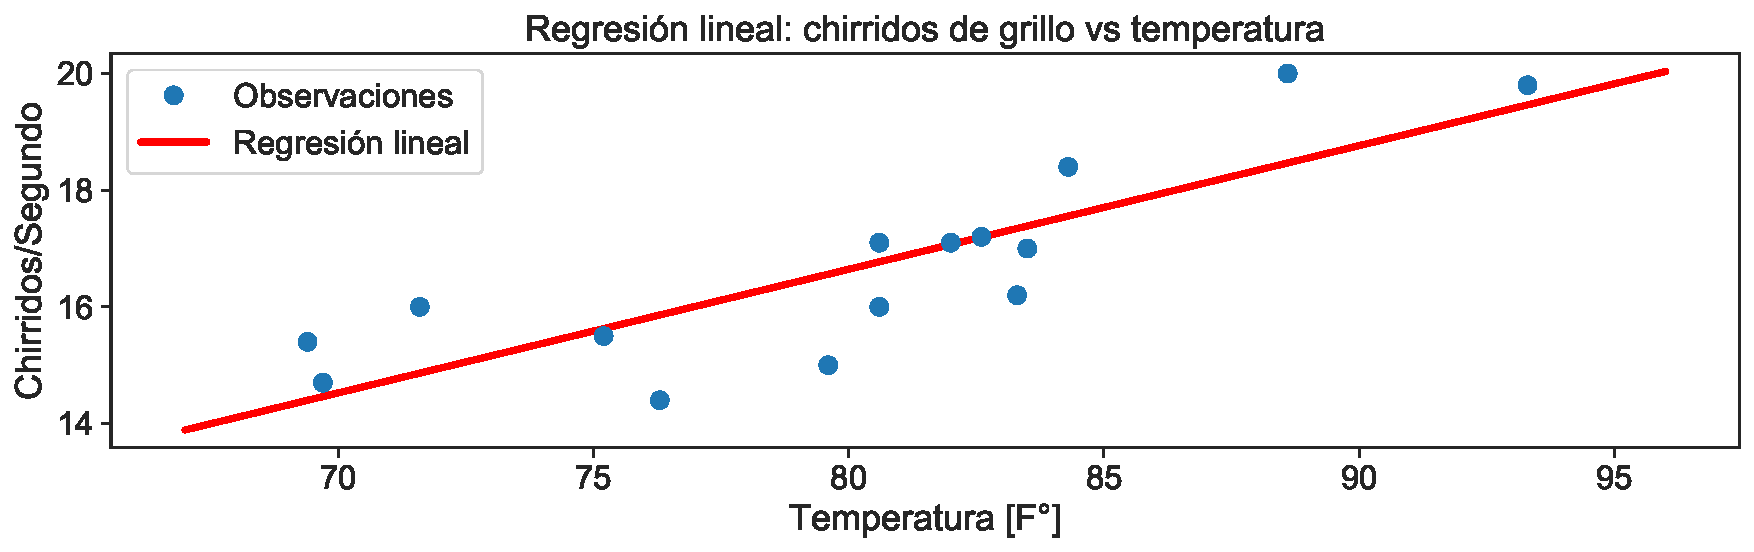
\includegraphics[width=0.9\textwidth]{img/cap1_chirridos.pdf}\\
	\caption{Ejemplo de regresión lineal.}
	\label{fig:reg_lin_1}
\end{figure}

La expresión $\left(\tX^\top\tX \right)^{-1} \tX^\top$ en la ecuación~\eqref{eq:sol_mse} es conocida como la pseudo-inversa de Moore-Penrose \cite[p.~7]{benisrael_greville_2006}. Observe que una condición necesaria para que esta pseudo-inversa esté bien definida es que la cantidad de observaciones ($N$) sea mayor o igual que las dimensiones ($M+1$). Esto es porque la matriz $\tX^\top\tX$ es de tamaño $(M+1)\times(M+1)$ y su rango es $\min \{N, M+1\}$, consecuentente, para que $\tX^\top\tX$ tenga rango completo (y por ende sea invertible) se debe cumplir al menos que $N\geq M+1$. Para encontrar una condición necesaria y suficiente para la existencia de la solución de mínimos cuadrados en la ecuación \eqref{eq:sol_mse}, además de el número de observaciones $N\geq M+1$ se requiere que éstas no sean colineales, pues de esta forma los términos que componen la pseudo-inversa son efectivamente linealmente independiente y ésta tiene rango completo. Es claro que para el caso de variables continuas es muy poco probable que dos observaciones sean perfectamente colinearles, sin embargo, en el caso de variables categóricas donde las observaciones son asignadas a un número finito de símbolos es probable que dos o más valores para la variable dependiente sean exactamente iguales. 

En la práctica, es usual que tengamos más observaciones que parámetros, cuando consideramos un modelo lineal (o lineal generalizado, como veremos a continuación). Sin embargo, es posible que las observaciones sean \emph{redundantes}, es decir, no exactamente iguales (y por ende linealmente independientes) pero suficientemente parecidas para que la inversa de Moore-Penrose esté \emph{cercana} a ser no invertible. Esto puede resultar en problemas de inestabilidad numérica al  calcular la inversa de $\tX^\top\tX$. Una forma de evitar este problema penalizar soluciones que son \emph{cercanas a ser no invertibles} o \emph{irregulares}, de forma similar que se penalizan funciones que no representan bien los datos, en el sentido del error cuadrático. Este procedimiento se refiere a \emph{regularizar} la solución.

\begin{mdframed}[style=pendiente, frametitle={\center ¿Por qué usamos el criterio de mínimos cuadrados?}]
1) Aproximación en $L^2$\\
2) Minimizar varianza del error, $x$ es variable aleatoria, $y=f(x)$ es determinista\\
3) Tanto $x$ como $y$ son variables aleatorias. Esperanza condicional.\\
4) Ejemplo: $X,Y$ conjuntamente gaussianos (definir MVN, contraejemplo, estimador óptimo). Analizar expresiones de la media y varianza posterior: interpretar.

	
\end{mdframed}


\begin{figure}[ht]
	\centering
	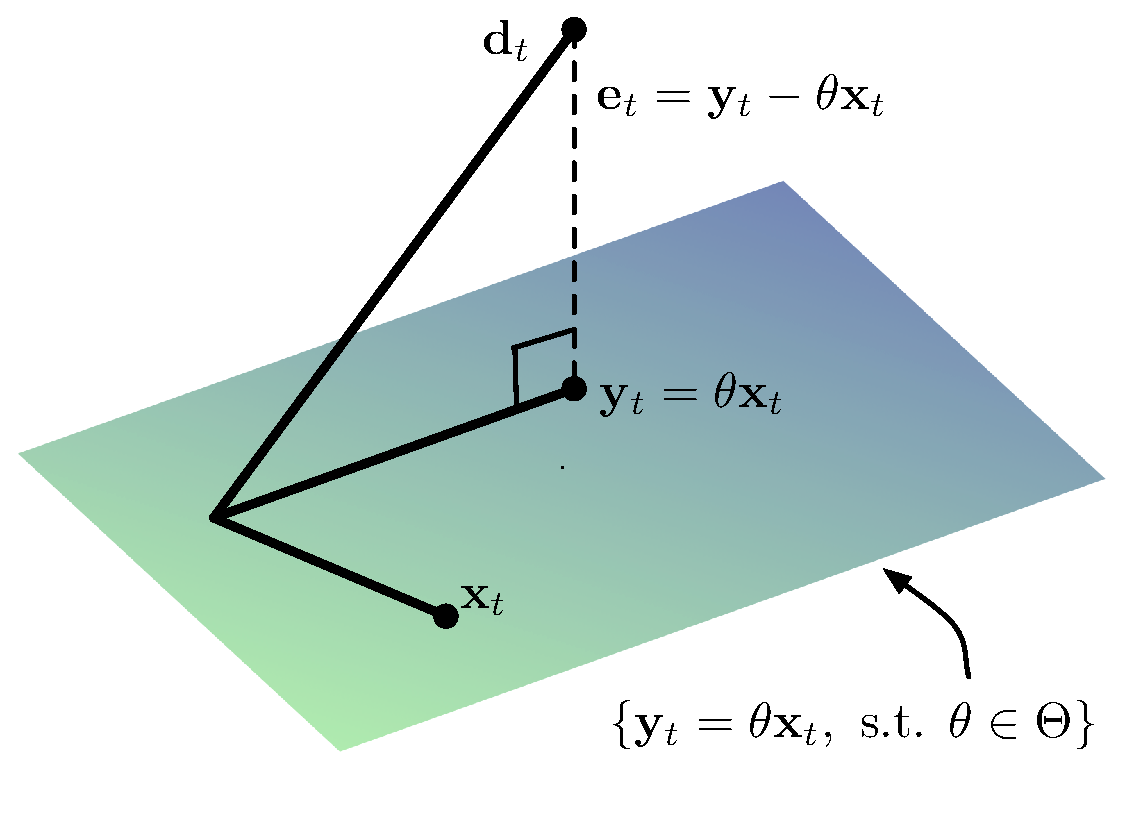
\includegraphics[width=0.5\textwidth]{img/projection.pdf}\\
	\caption{Interpretación geométrica de la regresión lineal y mínimos cuadrados}
	\label{fig:projection}
\end{figure}

% subsubsection Mínimos cuadrados (end)

\subsubsection{Mínimos cuadrados regularizados} % (fold)
\label{ssub:min_cuad_reg}

El criterio para encontrar los parámetros del modelo de regresión lineal puede, además de considerar el ajuste de la función a las observaciones, incluir ciertas penalizaciones sobre los modelos o soluciones a elegir. Estas penalizaciones pueden ser codificadas directamente en la función de costo, consecuentemente, ésta tiene ahora consta de un término que penaliza el ajuste de los datos y otro término que penaliza soluciones que se alejan de lo deseado. Un criterio estándar de penalización es la norma de los parámetros, es decir, 
\begin{equation}
	J_\rho = \frac{1}{2}\sum_{i=1}^N(y_i-\theta^
	\top \tx_i)^2 + \frac{\rho}{p}||\theta||_p^p,\ p\in\R_+,
	\label{eq:reg_least_squares}
\end{equation} 
donde $||\cdot||_p$ denota la norma $\ell_p$, es decir, $||\theta||_p=\left(\sum_{j=1}^N|\theta_j|^p\right)^\frac{1}{p}$ y el parámetro $\rho$ tiene el rol de balancear la importancia entre ajuste (primer término) y regularidad de la solución (segundo término). Distintos valores de $p$ inducen distintos propiedades sobre las soluciones, siendo las más usadas las correspondientes a $p=1$, conocido como \textbf{Lasso} \cite{tibshirani_1996}, y $p=2$ conocido como \textbf{regularización de Tikhonov} \cite{tikhonov_arsenin_1977} o bien \textbf{\emph{Ridge Regression}} \cite{hoerl_kennard_1970}.  

Una ventaja de la regularización de Tikhonov es que su solución, al igual que el caso de mínimos cuadrados no regularizados, puede ser encontrada en forma exacta. En efecto, para $p=2$ tenemos que el término de regularización puede ser expresado como $||\theta||_2 = \theta^\top\theta$, con lo que el minimizante del costo cuadrático regularizado está dado por: 
\begin{align}
\nabla_\theta J_\rho=0 &\Leftrightarrow \sum_{i=1}^N(\theta^\top \tx_i - y_i)\tx_i^\top + \rho\theta^\top=0  							&&\text{def. $J$}\\  
&\Leftrightarrow \sum_{i=1}^Ny_i\tx_i^\top = \sum_{i=1}^N\theta^\top \tx_i\tx_i^\top + \rho\theta^\top					&&\text{ordenar}\\
&\Leftrightarrow \theta^\top = \sum_{i=1}^Ny_i\tx_i^\top \left(\sum_{i=1}^N \tx_i\tx_i^\top + \rho \eye\right)^{-1}	&&\text{despejar $\theta^\top$}\\
&\Leftrightarrow \theta =  \left(\sum_{i=1}^N \tx_i\tx_i^\top +\rho \eye\right)^{-1} \sum_{i=1}^N \tx_i y_i 		&&\text{transponer}\\
&\Leftrightarrow \theta = \left(\tX^\top\tX +\rho \eye\right)^{-1} \tX^\top Y 											&&\text{def. $\tX$ y $Y$}
\end{align}

De la última expresión, es posible ver que el requerimiento de que las observaciones disponibles sean (i) más que la dimensión $M+1$ y que además (ii) éstas sean colineales ya no es necesario para que la solución esté bien definida. De hecho, la matriz $\tX^\top\tX$ puede efectivamente estar cercana a ser no invertible, sin embargo, es posible \emph{regularizar} la solución forzando que la matriz $\left(\tX^\top\tX +\rho \eye\right)$ sea efectivamente \emph{regular} aumentando el valor de $\rho$. 

En el caso de la regularización de Tikhonov, se entiende por soluciones regulares las que están definidas por parámetros que tienen una norma pequeña, tal como lo sugiere la ecuación \eqref{eq:reg_least_squares}. Sin embargo, es posible aplicar otros criterios de regularidad, por ejemplo, una solución regular puede ser una en la cual la mayoría de los de parámetros son idénticamente nulos, esto es conocido como una solución \textbf{rala} o \textbf{\emph{sparse}}. Usando por costo de regularización el número de parámetros no nulos (definido por la ``norma'' $l_0$) en la definición del costo en la ecuación \eqref{eq:reg_least_squares}, es posible determinar cuáles son las soluciones que utilizan menos variables independientes para representar la variable dependiente. Desafortunadamente, resolver encontrar la solución usando la ``norma'' $l_0$ es muy difícil, sin embargo, bajo ciertas condiciones la consideración de la norma $l_1$ puede llevar a la misma solución.

\begin{mdframed}[style=pendiente, frametitle={\center Regularización versus mínimos cuadrados}]
1) Referencias, Compressed sensing, sparse feature selection\\
2) ¿es justo comprar MC y RR en términos de MSE?\\
3) Elegir el coeficiente de regularización es crítico\\
4) Notar que la regularización mueve las estimaciones de los parámetros a cero, en particular RR manda a todos \emph{igualmente} a cero, sin fijar ninguno exactamente en cero. \\
5) cuando $\rho$ es suficientemente grande, lasso puede fijar parámetros exactamente cero, consecuentemente realizando \emph{selección de variables}\\
6) formulación con restricciones\\
7) interpretación geométrica\\
8) ¿cómo elegir $\rho$? y validación cruzada: subajuste, sobreajuste
\end{mdframed}

\subsubsection{Máxima verosimilitud} % (fold)
\label{ssub:max_ver}

Ahora tomaremos un enfoque distinto, en el cual no buscaremos el modelo \emph{aproximado} que tiene menor discrepancia con los datos. Por el contrario, nos enfocamos en modelos que han generado \emph{exactamente} los datos observados. Debido a la naturaleza de los datos, para este fin es necesario considerar modelos estocásticos, por lo que el mejor modelo estará dado por el que \emph{más probablemente} haya generado los datos. Específicamente, consideraremos un modelo compuesto por dos partes: la primera es determinística y paramétrica (al igual que los modelos anteriores) y una parte aleatoria la cual permitirá modelar exactamente las observaciones. 

En efecto, consideremos el siguiente modelo
\begin{equation}
	y = \theta^\top\tx + \epsilon,\quad \epsilon\sim\cN(0,\sigma_\epsilon^2) \ \text{i.i.d.},
	\label{eq:lin_gauss}
\end{equation}
donde la parte determinística ha sido elegida lineal en $\tx$ y la parte aleatoria es gaussiana. El modelo probabilístico en la ecuación~\eqref{eq:lin_gauss} puede expresarse en forma distribucional como 
\begin{equation}
	y|\tx \sim p(y|\tx,\theta) = \cN(y;\theta^\top\tx,\sigma_\epsilon^2).
\end{equation}

A diferencia del criterio de mínimos cuadradros, donde el entrenamiento del modelo (ajuste del parámetro $\theta$) se hacía en base a la función de pérdida cuadrática para un parámetro dado, en este caso el criterio de entrenamiento (en función de un conjunto de observaciones) es la \textbf{probabilidad de los datos} bajo el supuesto de un modelo dado o, equivalentemente, la \textbf{verosimilitud del modelo} dado los datos. Para aclarar este criterio, y antes de considerar optimización alguna, veamos que la verosimilitud del modelo lineal y gaussiano descrito arriba está dado, para un conjunto de observaciones $T=\{(x_i,y_i)\}_{i=1}^N$, por 
\begin{equation}
	l(\theta) \deq p(Y|\tX,\theta) = p(y_1,\ldots,y_N|\tx_1,\ldots,\tx_N,\theta)= \prod_{i=1}^Np(y_i|\tx_i,\theta) = \prod_{i=1}^N \cN(y_i;\theta^\top\tx_i,\sigma_\epsilon^2), \label{eq:verosimilitud}
\end{equation} 
donde la factorización de la probabilidad de los datos es posible dado que las observaciones son \textbf{condicionalmente independiente dado el modelo}.

El ajuste del modelo entonces puede entonces realizarse mediante la maximización (con respecto a $\theta$) de la función de verosimilitud $l(\theta)$ en la ecuación~\eqref{eq:verosimilitud}. Es decir: 
\begin{equation}
	\theta^{\text{MV}}= \argmax l(\theta),
\end{equation}
donde en superíndince ``MV'' denota ``máxima verosimilitud''. 

Para el caso lineal y gaussiano presentado en la ecuación~\eqref{eq:lin_gauss}, donde recordemos que las observaciones son condicionalmente independientes dado el modelo, el estimador $\theta^{\text{MV}}$ está dado por:
\begin{align}
	\theta^{\text{MV}} 	&= \argmax \prod_{i=1}^N \cN(y_i;\theta^\top\tx_i,\sigma_\epsilon^2) \\
						&= \argmax \prod_{i=1}^N \frac{1}{\sqrt{2\pi}\sigma_\epsilon} \exp\left({\frac{-1}{2\sigma_\epsilon^2}(y_i-\theta^\top\tx_i)^2}\right) \nonumber\\
						&= \argmin \sum_{i=1}^N (y_i-\theta^\top\tx_i)^2 \nonumber
\end{align}
Nótese que es posible identificar esta última expresión con la el costo cuadrático en la ecuación \eqref{eq:lin_least_squares2}, es decir, el estimador de máxima verosimilitud es el minimizante del mismo costo que el estimador de mínimos cuadrados. Consecuentemente, tenemos que ambos estimadores son iguales y de acuerdo a la ecuación \eqref{eq:sol_mse} dados por 
\begin{equation}
	\theta^{\text{MV}} = \theta^{\text{MC}} = \left(\tX^\top\tX +\rho \eye\right)^{-1} \tX^\top Y 
\end{equation}


\begin{mdframed}[style=discusion, frametitle={\center Discusión: A pesar de la equivalencia en el óptimo del parámetro, MV también permite optimizar la varianza del ruido}]
\end{mdframed}

\subsubsection{Regresión via inferencia bayesiana} % (fold)
\label{ssub:map}

\noindent\textbf{Tres pasos de inferencia bayesiana}
\begin{itemize}
	\item Definir un modelo conjunto para todas las cantidades involucradas, observaciones, valores futuros, parametros, etc
	\item Ajustar el modelo a la luz de observaciones
	\item Evaluar el modelo e interpretar resultados
\end{itemize}




En vez de maximizar la probabilidad de que los datos hayan sido generado por el modelo propuesto, podemos calcular la distribución condicional sobre modelos dado el conjunto de observaciones, es decir, $p(\theta|T)$. Esta es conocida como \emph{distribución posterior del modelo dado los datos} y mediante el teorema de Bayes puede expresarse como

\begin{equation}
	p(\theta|T)=\frac{p(Y|\theta,\tX)p(\theta,\tX)}{p(Y|\tX)}
	\label{eq:posterior}
\end{equation}

\noindent\textbf{Observaciones:}\\

\noindent 1) La constante de normalización es en general muy complicada de calcular, pues es la probabilidad de que la salida sea $Y$ para una entrada $\tx$ y \emph{cualquier} modelo, de hecho, 

\begin{equation}
		p(Y|\tX) 	= 	\int p(Y,\theta|\tX)\td \theta 
					= 	\int p(Y|\theta,\tX) p(\theta) \td \theta
\end{equation}

Sin embargo, nótese que $p(Y|\tX)$ es solo una constante de normalización y como $p(\theta|T)$ es una función de $\theta$, el denominador en ecuación~\eqref{eq:posterior} solo amplifica dicha función. Es decir 

\begin{equation}
	p(\theta|T)\propto p(Y|\theta,\tX)p(\theta,\tX)
	\label{eq:posterior2}
\end{equation}

La distribución posterior es entonces una \emph{mezcla} entre la distribución posterior (que representa la creencia en la variable antes de ver datos) y la verosimilitud (que representa la probabilidad de los datos condicional al modelo). Cuando la distribución a priori y a posteriori son de la misma familia, diremos que son distribuciones conjugadas y además que el prior es un \emph{prior} conjugado para la verosimilitud. Ejemplos de priors conjugados son las distribuciones gaussianas, por ejemplo, si consideramos $p(\theta,\tX) = \cN(0,\sigma_\theta^2)$ y una verosimilitud gaussiana (i.e., modelo linear con ruido gaussiano), tenemos

\begin{align}
	p(\theta|T)	&\propto p(Y|\theta,\tX)p(\theta,\tX)\\
				&= \cN(Y;\theta^\top\tX,\eye\sigma_\epsilon^2)\cN(\theta;0,\sigma_\theta^2)\\
				&=\cN(\theta; \mu,\Sigma)
\end{align}

\noindent\textbf{Observaciones:}\\
\noindent 1) ¿y la constante de normalización?

\doublebox{
\begin{minipage}{\linewidth}
\textbf{\underline{Ejemplo:}}

Otro caso de priors conjugados es la distribución binomial, que consiste en la probabilidad de obtener $s$ aciertos en $n$ intentos, cada uno independientes y equiprobables con probabilidad desconocida $q$.

\begin{equation}
	p(n, s) = \binom{n}{s} q^s (1-q)^{n-s}
\end{equation}

Donde su prior conjugado es la distribución Beta con parámetros ($\alpha, \beta$)

\begin{equation}
	p(q) = \frac{q^{\alpha-1}(1-q)^{\beta-1}}{\mathcal{B}(\alpha, \beta)}
\end{equation}

Donde $\mathcal{B}(x,y)$ es la función Beta que actua como factor normalizador.


Luego, si queremos obtener la posterior de $q$ con un prior Beta,

\begin{align}
	p(q|n,s) & = \frac{p(n.s|q)p(q)}{p(n,s)} \\
			 & = \frac{\binom{n}{s}q^s(1-q)^{n-s}q^{\alpha-1}(1-q)^{\beta-1}}{p(n,s)} \\
			 & = \textcolor{blue}{
			 \underbrace{\frac{\binom{n}{s}}{p(n,s)}
			 }}
			 q^s(1-q)^{n-s}q^{\alpha-1}(1-q)^{\beta-1}\\
			 & = \textcolor{blue}{\mathcal{B}(s+\alpha, \beta + n - s)} q^{s + \alpha-1} (1-q)^{n-s+\beta-1} && \text{Es una distribución Beta}
\end{align}
\textbf{\underline{Aplicación:}}

Se sabe que el $1\%$ de las mujeres tienen cancer de mamas, y se tiene un test para detectar si una mujer lo presenta o no. Si la paciente tiene cancer (C), el test dará postitivo (PT) con una probabilidad del $80\%$ y negativo (NT) con $20\%$, en cambio cuando la paciente está sana (NC), hay un $9.6\%$ de probabilidad que el test salga erroneo y si detecte cancer (PT).

Una paciente se realiza el test y este sale positivo, nos gustaría obtener la probabilidad de que en realidad tenga cancer dado este resultado.

\begin{align}
	p(C|PT) & =\frac{p(PT|C)p(C)}{p(PT)} \\
			& = \frac{p(PT|C)p(C)}{p(PT|C)p(C)+p(PT|NC)p(NC)} \\
			& = \frac{0.8 \cdot 0.01}{0.8 \cdot 0.01 + 0.096 \cdot 0.99}\\
			& = 0.0776
\end{align}

De esta misma forma podemos completar todos los casos.
\\
% \begin{table}%[H]
\centering
\begin{tabular}{c|cc}
\toprule
   & C ($1\%$) &  NC($99\%$) \\\hline
PT($10.3\%$) & $7.7\%$ & $92.3\%$\\
NT($89.6$\%) & $0.2\%$ & $99.8\%$ \\
\bottomrule
\end{tabular}
\captionof{figure}{Resumen de las probabilidades para el caso del test de cancer.}
\label{table:cancer}
% \end{table}

\end{minipage}}


% subsubsection máximo_a_posteriori (end)

\subsection{Maximo a posteriori} % (fold)
\label{sub:map}

¿Cuál es el equivalente a regularizar en es sentido probabilístico? La respuesta está en asignar más probabilidad \emph{a priori} antes de ver datos en vez de penalizar y encontrar (una) moda de la distribución posterior, es decir 


\begin{align}
	\theta_\text{MAP}^\star 	&= \argmax p(Y|\theta,\tX)p(\theta,\tX)\\
								&= \argmax \prod_{i=1}^Np(y_i|\tx_i,\theta)p(\theta,\tX)\\
								&= \argmax \prod_{i=1}^N \cN(y_i;\theta^\top\tx_i,\sigma_\epsilon^2)\cN(\theta;0,\sigma_\theta^2) \\
								&= \argmax \prod_{i=1}^N \frac{1}{\sqrt{2\pi}\sigma_\epsilon} \exp\left({\frac{-1}{2\sigma_\epsilon^2}(y_i-\theta^\top\tx_i)^2}\right)
											\frac{1}{(\sqrt{2\pi}\sigma_\theta)^{M+1}} \exp\left({\frac{-||\theta||^2}{2\sigma_\theta^2}}\right) \\
								&= \argmax  \frac{1}{\sqrt{2\pi}\sigma_\epsilon} \frac{1}{(\sqrt{2\pi}\sigma_\theta)^{M+1}}
											\exp\left( \sum_{i=1}^N{\frac{-1}{2\sigma_\epsilon^2}(y_i-\theta^\top\tx_i)^2} -{\frac{||\theta||^2}{2\sigma_\theta^2}}\right) \\
								&= \argmin \sum_{i=1}^N{(y_i-\theta^\top\tx_i)^2} +{\frac{\sigma_\epsilon^2}{\sigma_\theta^2}||\theta||^2}\quad {\tt (:|)}
\end{align}

\subsection{Predicciones} % (fold)
\label{sub:predicciones}
Una vez que el modelo está ajustado, ya sea con estimaciones paramétricas puntiales o distribucionales, ¿cómo hacemos predicciones? En el caso puntual, la predicción es simplemente evaluar el modelo en el parámetro encontrado $\theta$ y la entrada $x$. En el caso de la estimación bayesiana del parámetro, la predicción toma en cuenta todos los posibles valores del parámetro. En efecto, la distribución de la variable dependiente $y$ para una nueva entrada $x$ está dada por la distribución condicional del $y$ dado todos los datos de entrenamiento, es decir, 

\begin{equation}
 	p(y|x,\{(x_i,y_i)\}_{i=1}^N) = \int p(y|x, \theta)p(\theta|\{(x_i,y_i)\}_{i=1}^N) d\theta
 \end{equation} 

consecuentemente, la esperanza está dada por

\begin{align}
	\E{y|x,\{(x_i,y_i)\}_{i=1}^N} 
	&= \int y p(y|x,\{(x_i,y_i)\}_{i=1}^N) dy\\
	&= \int y p(y|x, \theta)p(\theta|\{(x_i,y_i)\}_{i=1}^N) d\theta dy\\
	&= \int y \cN(y;\theta^\top xp,\sigma_e^2)\cN(\theta;\mu_\theta, \sigma_\theta^2) d\theta dy\\
	&= \int \theta^\top x\cN(\theta;\mu_\theta, \sigma_\theta^2) d\theta \\
	&= \mu_\theta^\top x
\end{align}

% subsection predicciones (end)

\subsection{Ejercicios} % (fold)
\label{sub:ejercicios_regresion_lineal}

i) Considere el caso en que sus observaciones (entrada $x$, salida $y$) solo consisten en 
\begin{equation}
D = \{(1,a),(2,b)\}.
\end{equation}
Usando la expresión para la solución óptima de mínimos cuadrados de la ecuación \eqref{eq:sol_mse}, encuentre los parámetros del modelo lineal dado por 
\begin{equation}
	y = \theta_1 x +\theta_0 
\end{equation}
e interprete esta solución para distintos valores de $a$ y $b$.

ii) ¿Cuál es la estimador muestral de la covarianza entre $x$ e $y$ para las observaciones disponibles? 

ii) Interprete la correlación entre $x$ e $y$ 




\newpage
%!TEX root = notas_de_clase.tex

\section{Regresión No Lineal}
%El problema de regresión buscar encontrar la relación entre dos variables: entrada y salida, estímulo y respuesta, instancia y etiqueta, etc. El caso más simple, y que sirve de ilustración para modelos más expresivos es el de regresión lineal, donde dicha relación está restringida a ser lineal. 
El concepto de regresión lineal puede ser extendido para modelar relaciones no lineales entre variables de entrada y salida. Esto manteniendo los supuestos generales del modelo y la simpleza de la  solución de las ecuaciones que se desprenden. Para lograr esto se utiliza una familia de transformaciones no lineales.\\

Considere el conjunto de entrenamiento

\begin{equation}
	\{(x_i,y_i)\}_{i=1}^N,\quad (x_i, y_i)\in\R^M\times\R^1,\forall i=1,\ldots,N
	\label{eq:training_set_nl}
\end{equation}

Adicionalmente considere la función a valores vectoriales 
\begin{align}
  \Phi \colon \R^M &\to \R^D \nonumber\\
  x &\mapsto \Phi(x)=[\phi_1(x),\ldots,\phi_D(x)]
\end{align}
donde $\{ \phi_i \}_{j=1}^D$ son funciones escalares. \\

\noindent\textbf{Observaciones:}\\

\noindent 1) Nos referiremos a $\Phi(x)$ como \emph{características} y a $x$ simplementes como \emph{datos crudos}. \\

\noindent 2) La función $\Phi:x\mapsto\Phi(x)$ puede depender de parámentros, sin embargo, por ahora eso no es importante. \\

Usando el vector de características como entrada a un modelo lineal, podemos definir el siguiente modelo de regresión: 

\begin{equation}
    y = \Phi(x)\theta + \epsilon
\end{equation}
El cual puede ser escrito de forma vectorial de acuerdo a 
\begin{align}
    Y &= \Phi(X)\theta + \bepsilon\\
    Y &= [y_1,\ldots,y_N]^T \nonumber\\
    \Phi(X) &= \left[ \begin{matrix} \phi_1(x_1)& \ldots & \phi_D(x_1)\\
    \vdots & \ddots & \vdots \\
    \phi_1(x_N) & \ldots & \phi_D(x_N)\\
    \end{matrix} \right]
\end{align}

El ajuste, i.e., determinación de parámetros $\theta$ es entonces realizado mediante la minimización del siguiente funcional:
\begin{align}
    J &= \frac{1}{2} \sum_{i=1}^N(y_i - \Phi(x_i)\theta)^2\\
    &= \frac{1}{2} (Y-\Phi(X)\theta)^T(Y-\Phi(X)\theta)\\
    &= \frac{1}{2}Y^TY - \theta^T\Phi(X)^TY + \frac{1}{2}\theta^T\Phi(X)^T\Phi(X)\theta\\
\end{align}
El cual puede ser encontrado derivando $J$, es decir,

\begin{align}
    \frac{dJ}{d\theta} &= \Phi(X)^T\Phi(X)\theta - \Phi(X)^TY = 0\\
    \theta_{ML}&=\underset{\theta}{\argmin} J (\Phi(X)^T\Phi(X))^{-1}\Phi(X)^TY
\end{align}


De forma homologa al caso lineal, el caso regularizado es

\begin{equation}
    J_r = \frac{1}{2} \sum_{i=1}^N(y_i - \Phi(x_i)\theta)^2 + \rho\left \| \theta \right \|^2
\end{equation}

y su solución es

\begin{equation}
    \theta = (\Phi(X)^T\Phi(X)+\rho\mathbb{I})^{-1}\Phi(X)^TY
\end{equation}

\noindent\textbf{Observaciones:}

\noindent 1) Es importante notar que el modelo de regresión no lineal es \textbf{lineal en los parámetros}, no así en los datos.

\noindent 2) Como se mencionó anteriormente el modelo de regresión lineal es una generalización del caso lineal, esto es claro si se considera lo siguiente

\begin{align}
    \phi_0(x) &= 1, \phi_1(x) = x \nonumber\\
    \Phi &= [\phi_0, \phi_1] \nonumber\\
    \theta &= [\theta_0, \theta_1]^T \nonumber\\
    Y &= \Phi(X)\theta + \epsilon \nonumber
\end{align}

\noindent 3) La solución del caso no lineal $\theta_{nl} = (\Phi(X)^T\Phi(X))^{-1}\Phi(X)^TY$ es similar a la solución del caso lineal. Esto puede ser explicado por el hecho que hacer regresión no lineal con datos $\{(x_i,y_i)\}_{i=1}^N$ de $\R$ a $\R$, puede ser visto como una regresión lineal con datos $\{(\Phi(x_i),y_i)\}_{i=1}^N$ de $\R^D$ a $\R$.


\subsection{Bases de funciones}

La selección de la base de funciones es fundamental para el desempeño del método, si la familia de funciones no captura el comportamiento no lineal de los datos es muy improbable que el ajuste de la curva sea bueno. En general la elección de la base de funciones debe ser evaluada caso a caso.\\

A continuación se dan algunos ejemplos de bases de funciones que son usualmente utilizadas por su flexibilidad y/o simpleza.

\begin{itemize}
    \item{\textbf{Bases Polinomiales:}}
    La base es $\Phi=\{\phi_i\}_{i=0}^D$, donde $\phi_i(x)=x^i$, de esta forma
    
    \begin{equation}
        \Phi(X) = \left[ \begin{matrix} 1 & x_1 & x_1^2 & \ldots & x_1^D\\
        \vdots & \vdots & \vdots & \ddots & \vdots \\
        1 & x_N & x_N^2 & \ldots & x_N^D\\
        \end{matrix} \right]
    \end{equation}
    
    \item{\textbf{Bases Sinusoidales:}}
    La base es $\Phi=\{\phi_i\}_{i=0}^D$, donde 
    $\phi_i(x)=\cos(i\frac{2\pi}{2T}x)$, a medida que aumente $i$ mayor es la oscilación de la función, $T$ controla el periodo.
    
    \begin{equation}
        \Phi(X) = \left[ \begin{matrix}
        1 & \cos(i\frac{2\pi}{2T}x_1) & \ldots & \cos(D\frac{2\pi}{2T}x_1)\\
        \vdots & \vdots  & \ddots & \vdots \\
        1 & \cos(1\frac{2\pi}{2T}x_N) & \ldots & \cos(D\frac{2\pi}{2T}x_N)\\
        \end{matrix} \right]
    \end{equation}
    
    \item{\textbf{Escalones}}
    La siguiente base de funciones está compuesta funciones escalón que valen 1 dentro de un conjunto especifico y 0 en cualquier otro punto. Sean $c_1,c_2, \ldots,c_D$ una colección de valores crecientes, se define lo siguiente
    
    \begin{align}
        C_0(x) &= I_{(-\infty,c_1)}(x)\\
        C_i(x) &= I_{[c_i,c_{i+1})}(x), \quad \forall i=1,\ldots,D-1\\
        C_D(x) &= I_{[c_D,+\infty)}(x)\\
        I_A(x) &= \left\{\begin{matrix}
        1,\quad x\in A\\
        0,\quad x\notin A
        \end{matrix}\right.
    \end{align}
    
    De esta forma la base de funciones $\Phi=\{\phi_i\}_{i=0}^D$ queda definida por
    
    \begin{align}
        \phi_i(x) &= C_i(x),\quad \forall i=0,\ldots,D\\
        \Phi(X) &= \left[ \begin{matrix}
        1 & C_0(x_1) & \ldots & C_D(x_1)\\
        \vdots & \vdots  & \ddots & \vdots \\
        1 & C_0(x_N) & \ldots & C_D(x_N)\\
        \end{matrix} \right]
    \end{align}
    
    
    \item{\textbf{Polinomios por partes (Splines)}:}
    
    Una opción más flexible a hacer un ajuste polinomial en el dominio de los datos, es utilizar polinomios truncados definidos en intervalos, por ejemplo se puede ajustar
    
    \begin{equation}
        y = \left\{\begin{matrix}
        \beta_{01}+\beta_{11}x+\beta_{21}x^2+\beta_{31}x^3+\epsilon,\quad x < c\\
        \beta_{02}+\beta_{12}x+\beta_{22}x^2+\beta_{32}x^3+\epsilon,\quad x \geq c
        \end{matrix}\right.
    \end{equation}
    
    El problema con el modelo es que en el punto $c$ no existe ninguna restricción de continuidad. Para arreglar se considera la siguiente construcción.
    
    Se considera $\xi_1,\ldots,\xi_K$ una secuencia de puntos crecientes que serán los puntos en que cambia el régimen del polinomio, estos puntos se conocen como nudos. Ahora se define el polinomio truncado de grado $D$ con un nudo en $\xi_k$
    
    \begin{equation}
        (x-\xi_k)_+^D = \left\{\begin{matrix}
        0,\quad x < \xi_k\\
        (x-\xi_k)^D,\quad x \geq \xi_k
        \end{matrix}\right.
    \end{equation}
    
    Con esto polinomio truncado de grado $D$ y con $K$ nudos queda definido por
    
    \begin{equation}
        y = \beta_0 + \sum_{d=1}^D\beta_dx^d+\sum_{k=1}^K(x-\xi_k)_+^D
    \end{equation}
    
    \begin{equation}
        \Phi(X) = \left[ \begin{matrix} 1 & x_1 & x_1^2 & \ldots & x_1^D & \ldots & (x_1-\xi_1)_+^D & \ldots & (x_1-\xi_K)_+^D \\
        \vdots & \vdots & \vdots & \ddots & \vdots & \ddots & \vdots & \ddots & \vdots\\
        1 & x_N & x_N^2 & \ldots & x_N^D & \ldots & (x_N-\xi_1)_+^D & \ldots & (x_N-\xi_K)_+^D \\
        \end{matrix} \right]
    \end{equation}
    
\end{itemize}















\newpage
%!TEX root = notas_de_clase.tex

\subsection{Clasificación Lineal}

\subsubsection{Caso 2 clases}
%Dado un conjunto de datos en el plano donde cada punto pertenece a una dos categorías distintas $\mathcal{C}_1$ y $\mathcal{C}_2$, se quiere abordar el problema de clasificación utilizando un modelo lineal, el modelo más simple que se puede plantear es el siguiente:

\begin{minipage}{0.4\textwidth}
	Dado un conjunto de datos en el plano donde cada punto pertenece a una dos categorías distintas $\mathcal{C}_1$ y $\mathcal{C}_2$, se quiere abordar el problema de clasificación utilizando un modelo lineal, el modelo más simple que se puede plantear es el siguiente:
	
	\begin{equation}
		y(x) = \theta^Tx + w
	\end{equation}
	
	Este modelo funciona de la siguiente manera, $x$ será asignado a $\mathcal{C}_1$ si $y(x) \geq 0$ y será asignado $\mathcal{C}_2$ en el caso contrario.
\end{minipage}\hfill
%[AGREGAR IMAGEN]
\begin{minipage}{0.5\textwidth}
	\centering
	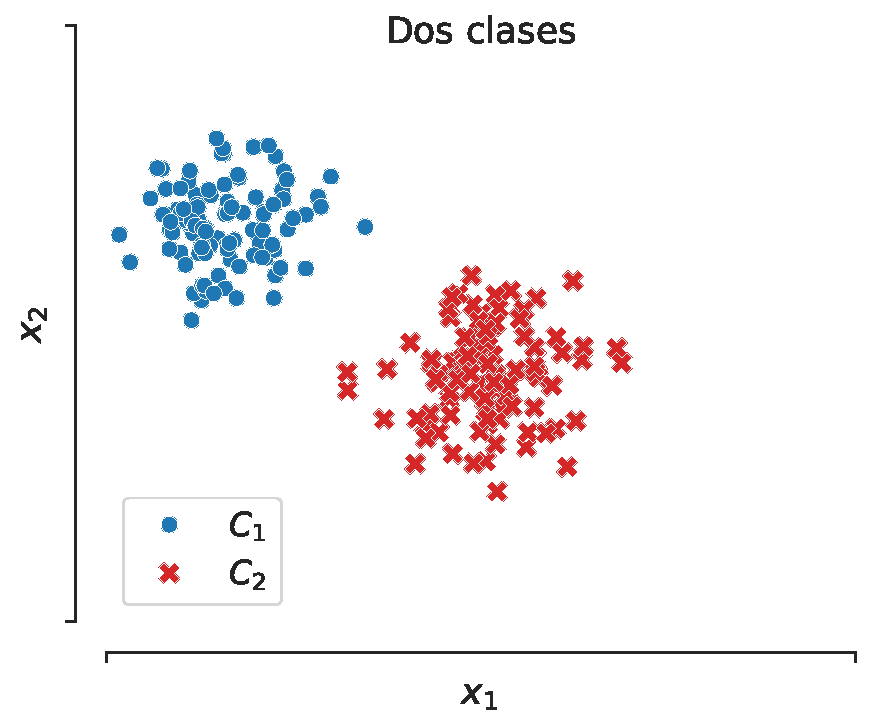
\includegraphics[width=0.8\textwidth]{img/cap2_dosclases}\\
	\captionof{figure}{Ejemplo de datos, los puntos\\ en azul pertenecen a $\mathcal{C}_1$, los rojos a $\mathcal{C}_2$.}
	\label{fig:puntos_2d}
\end{minipage}

\vspace{1cm}
La superficie de decisión queda definida por $y(x)=0$, si $x\in\R^D$, entonces la superficie de decisión corresponde a un hiperplano de dimensión $D-1$.

Sean $x_1,x_2$ dos puntos en la superficie de decisión, entonces se cumple lo siguiente:

\begin{align}
	0 &= y(x_1) - y(x_2) \nonumber\\
	  &= \theta^Tx_1 + w - \theta^Tx_2 - w \nonumber\\
	  &= \theta^T(x_1-x_2)
\end{align}

Esto muestra que $\theta$ es ortogonal a cualquier vector que esté contenido dentro del hiperplano de decisión, esto nos dice que el vector $\theta$ controla la inclinación del hiperplano.

Por otro lado, si $y(x)=0$:

\begin{equation}
	\frac{\theta^Tx}{\left \| \theta \right \|} = -\frac{w}{\left \| \theta \right \|}
\end{equation}

Esto muestra que la distancia normal de un punto $x$ en la superficie de decisión al origen está dada por el parámetro $w$.

Más aun $y(x)$ da una media con signo sobre cuanto es la distancia perpendicular $r$ entre el punto $x$ y la superficie de decisión. Dado cualquier punto $x$, este puede ser descompuesto en su proyección ortogonal sobre la superficie de decisión $x_{\bot}$ y la componente restante respecto al vector $\theta$, de forma que:

\begin{align}
	x &= x_{\bot}+r\frac{\theta}{\left \| \theta \right \|}\\
	y(x) &= \theta^Tx+w\\
	&= \theta^Tx_{\bot} + r\frac{\theta^T\theta}{\left \| \theta \right \|} + w\\
	\Rightarrow \quad r &= \frac{\theta^T+w}{\left \| \theta \right \|} 
	= \frac{y(x)}{\left \| \theta \right \|}
\end{align}

\newpage
\subsubsection{Caso multi clase}

Si se tienen $K$ clases $\mathcal{C}_k$ distintas, un enfoque posible para abordar el problema de clasificación es considerar $K$ discriminantes lineales.

\begin{equation}
	y_k(x) = \theta_k^Tx + w_k, \quad k=1,\ldots,K
\end{equation}

Donde $x$ será asignado a la clase $\mathcal{C}_k$ si y solo si $y_k(x) > y_j(x),\quad \forall j\neq k$, es decir:

\begin{equation}
	\mathcal{C}(x) = \underset{k}{\argmax}\hspace{1mm} y_j(x)
\end{equation}

\subsubsection{Clasificación con mínimos cuadrados}

Ya planteado el modelo, la pregunta que queda por responder pasa a ser como determinar $\theta$ y $w$, dado los métodos presentados en las clases anteriores el enfoque de mínimos cuadrados parece una respuesta natural a este problema, en primer lugar se introducirá un poco de notación para plantear el problema de una forma cómoda.

Dadas $\{\mathcal{C}_k\}_{k=1}^K$ clases distintas y un punto $x$ usaremos el vector $t\in\{0,1\}^K$ para codificar la pertenencia de $x$ a una clase especifica, por ejemplo: si $x\in\mathcal{C}_j$ entonces el vector $t$ asociado estará compuesto 

\begin{equation}
	x\in\mathcal{C}_j \Leftrightarrow t_j=1 \wedge t_i=0, \quad i\neq j
\end{equation}

esta codificación también es conocida como 'one-hot'.

Cada clase $\mathcal{C}_k$ posee su propio modelo lineal:

\begin{equation}
	y_k(x) = \theta_k^Tx + w_k \nonumber
\end{equation}

El sistema puede ser reescrito de forma matricial como:

\begin{equation}
	y(x) = \tilde{\Theta}^T\tilde{x}
\end{equation}

Donde la $K$-esima columna de $\tilde{\Theta}$ es un vector de $D+1$ dimensiones definido por $\tilde{\theta}=(w_k, \theta_k^T)^T$ y $\tilde{x}=(1,x^T)^T$ corresponde al vector $x$ aumentado. De esta forma un punto $x$ será asignado a la clase que tenga mayor $y_k=\tilde{\theta}_k^T\tilde{x}$.

Considerando un conjunto de entrenamiento $\{x_n,t_n\}_{n=1}^N$, definimos las siguientes matrices:

\begin{align}
	T &= [t_1, t_2,\ldots, t_N]^T\\
	\tilde{X} &= [\tilde{x}_1, \tilde{x}_2, \ldots, \tilde{x}_N ]^T
\end{align}

Finalmente para determinar los coeficientes de $\tilde{\Theta}$, minimizamos la suma de los errores cuadráticos de forma similar al problema de regresión, la función de costo puede ser escrita de la siguiente manera:

\begin{equation}
	E_D(\tilde{\Theta}) = Tr\{(\tilde{\Theta}\tilde{X}-T)^T(\tilde{\Theta}\tilde{X}-T)\}
\end{equation}

Donde $Tr$ corresponde al operador traza, al derivar e igualar a 0 la expresión (92), la solución es:

\begin{equation}
	\tilde{\Theta} = (\tilde{X}^T\tilde{X})^{-1}\tilde{X}T = \tilde{X}^*T
\end{equation}

Donde $\tilde{X}^*$ denota la pseudo-inversa de la matriz $\tilde{X}$, finalmente la solución es:

\begin{equation}
y(x) = T^T(\tilde{X}^*)\tilde{x}
\end{equation}

El problema con este enfoque es que mínimos cuadrados es muy sensible a la presencia de puntos aislados, dada la penalización cuadrática, los puntos lejanos al promedio de los datos tiene una influencia mucho mayor, lo que puede empeorar considerablemente los resultados.


\begin{figure}[H]
	\centering
	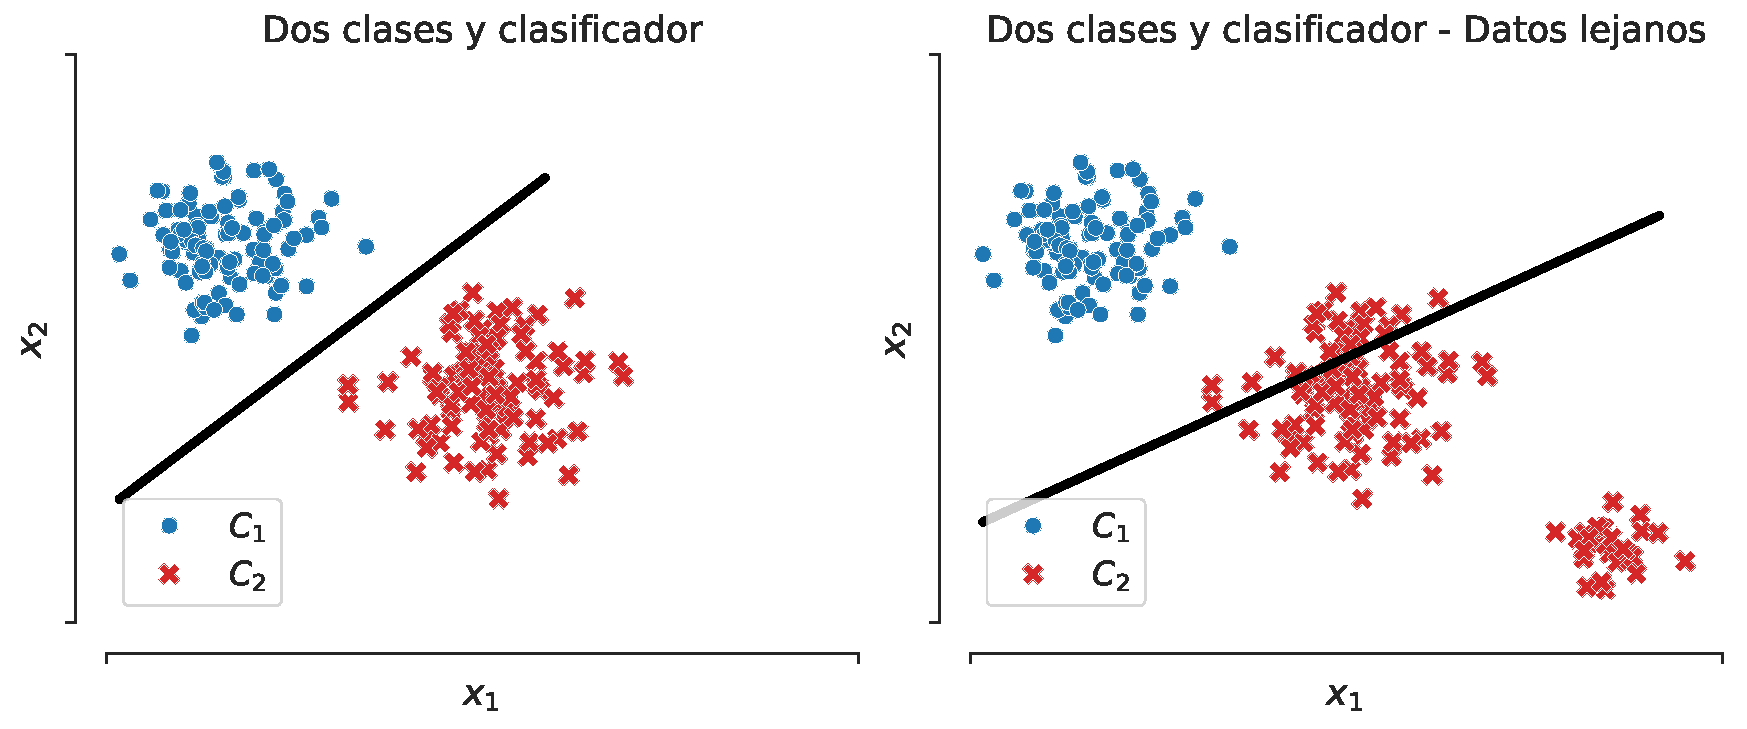
\includegraphics[width=0.7\textwidth]{img/cap2_dosclases_clasificador.pdf}\\
	\caption{Ejemplo ilustrativo sobre como los puntos lejanos pueden afectar negativamente los resultados.}
	\label{fig:clasif_mse}
\end{figure}

\subsubsection{Discriminante lineal de Fisher}

Una forma de ver un modelo de clasificación es en termino de reducción de dimensionalidad. Consideremos el caso en que hay 2 clases y un vector $x\in R^D$ que proyectamos a 1 dimensión de la siguiente manera:

\begin{equation}
	y = \theta^Tx
\end{equation}

Si definimos un umbral $w$, asignamos $x$ a $\mathcal{C}_1$ si $y\geq-w$ y $x$ a $\mathcal{C}_2$ en el caso contrario, recuperamos el modelo lineal que se discutido a través de esta capítulo.

En general al proyectar $D$ dimensiones a 1 se pierde gran cantidad de la información, esto se expresa en el hecho que clases claramente separadas en el espacio $D$-dimensional pueden traslaparse al ser proyectadas a 1 dimensión. Sin embargo al ajustar las componentes de $\theta$, podemos seleccionar una proyección que maximice la separación entre clases.

Para comenzar sean $N_1 = |\mathcal{C}_1|$ y $N_2 = |\mathcal{C}_2|$, con esto calculamos los promedios por clase.

\begin{equation}
	\text{m}_1=\frac{1}{N_1}\sum_{n\in\mathcal{C}_1}x_n
	\quad\quad\quad
	\text{m}_2=\frac{1}{N_2}\sum_{n\in\mathcal{C}_2}x_n
\end{equation}

La medida más simple de separación entre las clases cuando son proyectadas sobre $\theta$ es la separación entre los promedios de clase, esto sugiere elegir un $\theta$ que maximice la siguiente expresión

\begin{equation}
	m_1 - m_2 = \theta^T(\text{m}_1-\text{m}_2)
\end{equation}

Donde $m_k= \theta^T\text{m}_k$ corresponde al promedio de la clase $\mathcal{C}_k$ proyectado sobre $\theta$. Esta expresión puede ser arbitrariamente grande si escalamos $\theta$, para evitar imponemos que $\left \| \theta \right \|_2=1$. Usando multiplicadores de Lagrange para optimizar el problema restringido se llega a que $\theta\propto(\text{m}_1-\text{m}_2)$. El problema con esta solución es que pueden existir 2 clases bien separadas en el espacio $D$-dimensional, pero al proyectar los datos sobre la recta que une sus promedios, las proyecciones de cada clase se traslapen.

\begin{figure}[H]
	\centering
	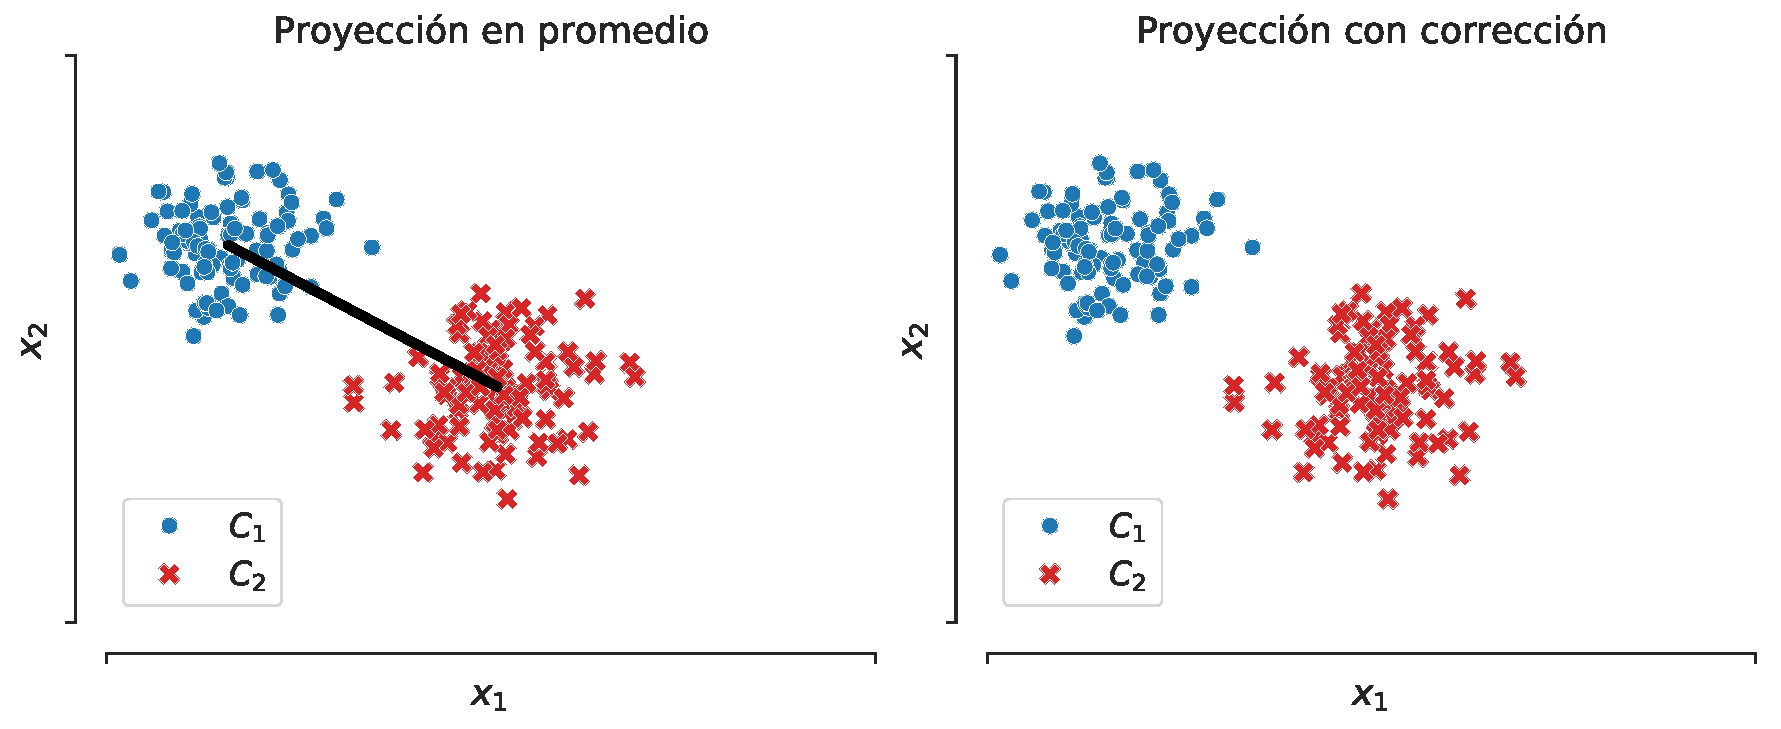
\includegraphics[width=0.7\textwidth]{img/cap2_dos_clases_proyeccion.pdf}\\
	\caption{(a) Resultado obtenido al proyectar sobre la recta que une los promedios de cada clase. (b) Resultado al considerar una corrección que considera minimizar la dispersión entre clases.}
	\label{fig:ej_fda}
\end{figure}

Para resolver este problema Fisher propuso maximizar una función que de como resultado una gran separación entre clases distintas, pero que al mismo tiempo minimice la separación dentro de una misma clase, de esta forma el traslape entre clases disminuye. 

Definimos la varianza dentro una clase como:

\begin{align}
	s_k^2 &= \sum_{n\in \mathcal{C}_k}(\theta^T(x_n-\text{m}_k))^2\\
	&= \sum_{n\in \mathcal{C}_k}(y_n-m_k)^2
\end{align}
Con esto se define la nueva función objetivo de la siguiente manera:

\begin{equation}
J(\theta) = \frac{m_1-m_2}{s_1^2+s_2 ^2}
\end{equation}

Podemos usar la ecuaciones descritas anteriormente para escribir $J(\theta)$ de forma explicita respecto a $\theta$.

\begin{equation}
	J(\theta) = \frac{\theta^TS_B\theta}{\theta^TS_W\theta}
\end{equation}

Donde $S_B$ es la matriz de covarianza entre clases dada por:

\begin{equation}
	S_B = (\text{m}_1-\text{m}_2)(\text{m}_1-\text{m}_2)^T
\end{equation}

$S_W$ es la matriz total de covarianza dentro de clases, dada por:

\begin{equation}
	S_W = \sum_{n\in \mathcal{C}_1}(x_n-\text{m}_1)(x_n-\text{m}_1)^T+
	\sum_{n\in \mathcal{C}_2}(x_n-\text{m}_2)(x_n-\text{m}_2)^T
\end{equation}

Al derivar $J(\theta)$ se encuentra que la función es maximizada cuando:

\begin{equation}
	(\theta^TS_B\theta)S_W\theta = (\theta^TS_W\theta)S_B\theta
\end{equation}

Por la definición de $S_B$, vemos que $S_B\theta$ es co-lineal con $(\text{m}_1-\text{m}_2)$. Más aun no es importante la norma de $\theta$, solo interesa la orientación, por esta razón descartamos los escalares $(\theta^TS_B\theta)$ y $(\theta^TS_W\theta)$, al despejar $\theta$ vemos que la solución es:

\begin{equation}
	\theta \propto S_W^{-1}(\text{m}_1-\text{m}_2)
\end{equation}
\newpage
\subsection{Clasificación No Lineal}

\subsubsection{El Perceptrón}

El perceptrón de Rosenblatt es un modelo de clasificación binario que tuvo mucha importancia en el área de reconocimiento de patrones. El modelo consiste en una función no-lineal fija usada para transformar $x$ en un vector de características $\phi(x)$, que luego es usado para generar un modelo lineal generalizado de la siguiente forma:

\begin{align}
	y(x) &= f(\theta^T\phi(x))\\
	f(a) &= \left\{\begin{matrix}
	+1,\quad a\geq 0\\
	-1,\quad a<0
	\end{matrix}\right.
\end{align}

Típicamente el vector $\phi(x)$ contiene un intercepto para la recta, es decir $\phi_0\equiv1$. El modelo asigna $x$ a la clase $\mathcal{C}_1$ si $y(x)=+1$ y asignará $x$ a la clase $\mathcal{C}_2$ cuando $y(x)=-1$.

Para encontrar el vector $\theta$ suele usarse un criterio basado en los datos que fueron clasificados incorrectamente llamado el criterio del perceptrón, este puede deducirse notando que se quiere encontrar un vector de pesos $\theta$ tal que para los $x\in\mathcal{C}_1$ cumpla $\theta^T\phi(x) > 0$ y para los $x\in\mathcal{C}_2$ cumpla $\theta^T\phi(x) < 0$, usando el hecho que $y(x)\in\{1,-1\}$, ambas condiciones pueden ser cubiertas por la expresión:

$$\theta^T\phi(x)y(x) > 0,\quad \forall x \in \mathcal{C}_1\cap\mathcal{C}_2$$

El criterio del perceptrón asocia a los puntos clasificados correctamente 0 error y a los puntos mal clasificados error $-\theta^T\phi(x)y(x)$, de esta forma si denotamos como $\mathcal{M}$ el conjunto de puntos mal clasificados, se debe minimizar la siguiente función objetivo:

$$ E_p(\theta) = -\sum_{i\in\mathcal{M}}\theta^T\phi(x_i)y(x_i) $$

Para minimizar esta función se usa descenso de gradiente estocástico, las actualizaciones son de la siguiente manera:

\begin{align}
	\theta^{\tau+1} &= \theta^\tau - \eta \nabla E_p(\theta)\\
	&= \theta^\tau + \eta \phi(x_n)y(x_n)
\end{align}

La constante $\tau$ corresponde a un entero que indexa las iteraciones. Por otra lado $\eta$ es una constante que se conoce como tasa de aprendizaje, dado que la función del perceptŕon $y(x)=y(x,\theta)$ no cambia si se multiplica $\theta$ por una constante cualquiera, sin perdida de generalidad podemos asumir que $\eta=1$. Es importante notar que al actualizar el vector $\theta$, el conjunto de puntos mal clasificados $\mathcal{M}$ va a cambiar.

La interpretación del algoritmo usado para ajustar el perceptrón es simple, se recorre el conjunto de puntos de entrenamiento $\{x_n\}_{n=1}^N$, si el punto $x_n$ fue clasificado correctamente el vector de pesos de mantiene igual, por otro lado si $x_n$ fue clasificado incorrectamente, el vector $\theta^\tau$ es actualizado según (89).
\newpage
\subsubsection{Clasificación Probabilista}

Los modelos que hemos mencionado anteriormente son de tipo discriminativo, es decir modelan directamente la probabilidad condicional $\mathbb{P}(\mathcal{C}_k|x)$, que da la probabilidad de pertenencia a una clase dado un dato.

Otro paradigma más poderoso a considerar es un enfoque generativo en el cual modelamos $\mathbb{P}(x|\mathcal{C}_k)$ junto con un prior $\mathbb{P}(\mathcal{C}_k)$ para las clases, luego podemos calcular la densidad posterior usando el Teorema de Bayes.

\begin{equation}
	\mathbb{P}(\mathcal{C}_k|x) = \frac{\mathbb{P}(x|\mathcal{C}_k)\mathbb{P}(\mathcal{C}_k)}{\mathbb{P}(x)}
\end{equation}

Considere el siguiente desarrollo, para el caso con 2 clases:

\begin{align}
	\mathbb{P}(\mathcal{C}_1|x) &= \frac{\mathbb{P}(x|\mathcal{C}_1)\mathbb{P}(\mathcal{C}_1)}{\mathbb{P}(x)}\\
	&= \frac{\mathbb{P}(x|\mathcal{C}_1)\mathbb{P}(\mathcal{C}_1)}{\mathbb{P}(x|\mathcal{C}_2)\mathbb{P}(\mathcal{C}_2)+\mathbb{P}(x|\mathcal{C}_1)\mathbb{P}(\mathcal{C}_1)}\\
	&=\frac{1}{1+\frac{\mathbb{P}(x|\mathcal{C}_1)\mathbb{P}(\mathcal{C}_1)}{\mathbb{P}(x|\mathcal{C}_2)\mathbb{P}(\mathcal{C}_2)}}\\
	&=\frac{1}{1+\exp(-a)} = \sigma(a)\\
\end{align}

Donde $a = \ln(\frac{\mathbb{P}(x|\mathcal{C}_1)\mathbb{P}(\mathcal{C}_1)}{\mathbb{P}(x|\mathcal{C}_2)\mathbb{P}(\mathcal{C}_2)})$.

\begin{itemize}
	\item La función logística está se define como $\sigma(a) = \frac{1}{1+e^{-a}}$.
	
	\item Tiene propiedades útiles como $\sigma(-a)=1-\sigma(a)$ y $\frac{d}{da}\sigma(a)=\sigma(a)(1-\sigma(a))$
	
	\item La inversa de la función logística se conoce como logit y es definida por $a(\sigma)=\ln(\frac{\sigma}{1-\sigma})$
\end{itemize}

Para el caso multi-clase, se puede hacer un desarrollo similar:

\begin{align}
	\mathbb{P}(\mathcal{C}_i | x) &= \frac{\mathbb{P}(x | \mathcal{C}_i)\mathbb{P}(\mathcal{C}_i)}{\sum_{j\neq i}\mathbb{P}(x | \mathcal{C}_j)\mathbb{P}(\mathcal{C}_j)}\\
	&= \frac{\exp(a_i)}{\sum_{j\neq i}\exp(a_j)}\\
	a_i &= \mathbb{P}(x | \mathcal{C}_i)\mathbb{P}(\mathcal{C}_i)
\end{align}

La función que aparece se conoce como softmax y corresponde a una generalización de la función logística a más dimensiones, adicionalmente tiene la propiedad de ser una aproximación suave de la función máximo.

\newpage

\noindent{\textbf{-Ejemplo:}} Normal class-conditional densities

Suponemos que las densidades condicionales de clase distribuyen como una normal multivariada, $p(x|\mathcal{C}_k) \sim \mathcal{N} (\mu_k,\Sigma)$ :

\begin{align}
p(x|\mathcal{C}_k)&=\frac{1}{(2\pi)^\frac{D}{2}|\Sigma|^\frac{1}{2}}\exp(-\frac{1}{2}(x-\mu_k)^T\Sigma^{-1}(x-\mu_k))\\
\Rightarrow \quad a &= \ln(\exp(-\frac{1}{2}(x-\mu_1)^T\Sigma^{-1}(x-\mu_1) +\frac{1}{2}(x-\mu_2)^T\Sigma^{-1}(x-\mu_2)))\\
&= \theta^Tx+w
\end{align}

Donde:

\begin{align}
\theta &= \Sigma^{-1}(\mu_1-\mu_2)\\
w &= \frac{1}{2}(\mu_1^T\Sigma^{-1}\mu_1+\mu_2^T\Sigma^{-1}\mu_2)
+\ln(\frac{p(\mathcal{C}_1)}{p(\mathcal{C}_1)})\\
\Rightarrow \quad p(\mathcal{C}_k|x) &= \sigma(\theta^Tx+w)
\end{align}

¿Como ajustar los parámetros de las condicionales a la clase y priors respectivamente?

\begin{itemize}
	\item\textbf{Parámetros:}
	\begin{align}
	p(\mathcal{C}_1)&=\pi \quad \Rightarrow \quad p(\mathcal{C}_2)=1-\pi\\
	p(x|\mathcal{C}_k) &= \mathcal{N}(\mu_k,  \Sigma); k=1,2
	\rightarrow \mu_1,\mu_2,\Sigma
	\end{align}
	
	\item\textbf{Datos:}
	\begin{align}
	T&=(t_1,t_2,\ldots,t_N) \in \{0,1\}^N\\
	X&=(x_1,x_2,\ldots,x_N)
	\end{align}
	
	\item\textbf{Likelihood:}
	
	Se recuerda que $p(x,\mathcal{C}_k)=p(x|\mathcal{C}_k)p(\mathcal{C}_k)=p(\mathcal{C}_k)\mathcal{N}(x|\mu_k,\Sigma)$, se procede a calcular la función de verosimilitud de los datos:
	
	\begin{align}
	p(X,T|\pi,\mu_1,\mu_2,\Sigma) &= \prod_{i=1}^{N}p(x_i,t_i|\pi,\mu_1,\mu_2,\Sigma)\\
	&= \prod_{i=1}^{N}p(x_i,\mathcal{C}_1)^{t_i}p(x_i,\mathcal{C}_0)^{1-t_i}\\
	&= \prod_{i=1}^{N}(\pi\mathcal{N}(x_i|\mu_1,\Sigma))^{t_i}
	((1-\pi)\mathcal{N}(x_i|\mu_2,\Sigma))^{1-t_i}
	\end{align}
	
	Más facil que el likelihood, es log-likelihood:
	
	\begin{equation}
	\log(L) := \sum_{i=1}^{N}t_i(\log(\pi)+\log(\mathcal{N}(x_i|\mu_1,\Sigma)))+(1-t_i)(\log(1-\pi)+\log(\mathcal{N}(x_i|\mu_2,\Sigma)))
	\end{equation}
	
	\newpage
	\noindent \textbf{1)}Derivada con respecto a $\pi$:
	
	\begin{align}
	\frac{\partial\log(L)}{\partial\pi} &= \sum_{i=1}^N \frac{t_i}{\pi}+\frac{1-t_i}{1-\pi}=0\\
	\Rightarrow \quad & (i-\pi)\sum_{i=1}^Nt_i = \pi\sum_{i=1}^N(1-t_i)\\
	\Rightarrow \quad & \sum_{i=1}^Nt_i=\pi N \quad\Rightarrow\quad \pi = \frac{\sum_{i=1}^Nt_i}{N} = \frac{N_1}{N_1+N_2}
	\end{align}
	
	Observamos que el valor encontrado para $\pi$ corresponde al promedio de las clases.
	
	\noindent \textbf{2)}Derivada con respecto a $\mu_1$:
	
	\begin{align}
	\frac{\partial\log(L)}{\partial\mu_1} &= \sum_{i=1}^N t_i
	\frac{\partial}{\partial \mu_1}(-\frac{1}{2}(x_i-\mu_1)^T\Sigma^{-1}(x_i-\mu_1))\\
	&= \sum_{i=1}^N t_i(\Sigma^{-1}(x_i-\mu_1)) =
	\Sigma^{-1}\sum_{i=1}^N t_i(x_i-\mu_1) = 0\\
	\Rightarrow\quad & \sum_{i=1}^Nt_ix_i= \mu_1\sum_{i=1}^N t_i
	\quad\Rightarrow\quad \mu_1 = \frac{1}{N_1}\sum_{i=1}^Nt_ix_i
	\end{align}
	
	De forma análoga:
	\begin{equation}
	\mu_2 = \frac{1}{N_2}\sum_{i=1}^N(1-t_i)x_i
	\end{equation}
	
\end{itemize}

\subsubsection{Regresión Logística v/s Modelo Generativo}

Los supuestos hechos sobre el modelo generativo resultaron en:

\begin{equation}
p(\mathcal{C}_1|x) = \sigma(w^Tx) = \frac{1}{1+e^{-w^Tx}}
\end{equation}

Encontrar $w$ de forma directa es mucho más fácil que ajustar todos los parámetros del modelo generativo.

Para dejar este punto en claro, se calculará la verosimilitud de la regresión logística con datos $\{x_i,y_i\}_{i=1}^N$, para hacer la notación más compacta denotamos $\sigma_i = \sigma(w^Tx_i)$.


\begin{align}
p(y_{1:N}|x_{1:N},w) &= \prod_{i=1}^{N}p(y_i|x_i,w)\\
&= \prod_{i=1}^{N}\sigma_i^{y_i}(1-\sigma_i)^{1-y_i}\\
NLL &= -\log(p(y_{1:N}|x_{1:N},w))\\
&= -\sum_{i=1}^N y_i\log(\sigma_i) + (1-y_i)\log(1-\sigma_i)
\end{align}

Se procede a calcular el gradiente de $NLL$ respecto a $w$:

\begin{align}
\nabla_w NLL &= -\sum_{i=1}^N y_i\frac{\sigma_i(1-\sigma_i)}{\sigma_i}x_i
+ (1-y_i)\frac{-\sigma_i(1-\sigma_i)}{\sigma_i}x_i\\
&= -\sum_{i=1}^N y_i(1-\sigma_i)x_i - (1-y_i)\sigma_ix_i\\
&= \sum_{i=1}^N (\sigma_i-y_i)x_i
\end{align}\newpage
%!TEX root = notas_de_clase.tex

\newpage
\centerline{--------------------------------- clase X/4/18 ---------------------------------}
\section{Selección de Modelo}
Supongamos que tenemos un montón de datos, de los cuales podemos ajustar un millón de modelos, tanto como la imaginación nos limite. Entonces ¿Con cuál te quedarías al final?
Cuando nos enfrentamos a la decisión de elegir un modelo usualmente lo que más interesa es la preciso del modelo a la hora de generalizar. El problema de solo buscar precisión es claro: \emph{overfitting} (ver figura \ref{fig:overfitting}).
\begin{figure}[h!]
    \centering
    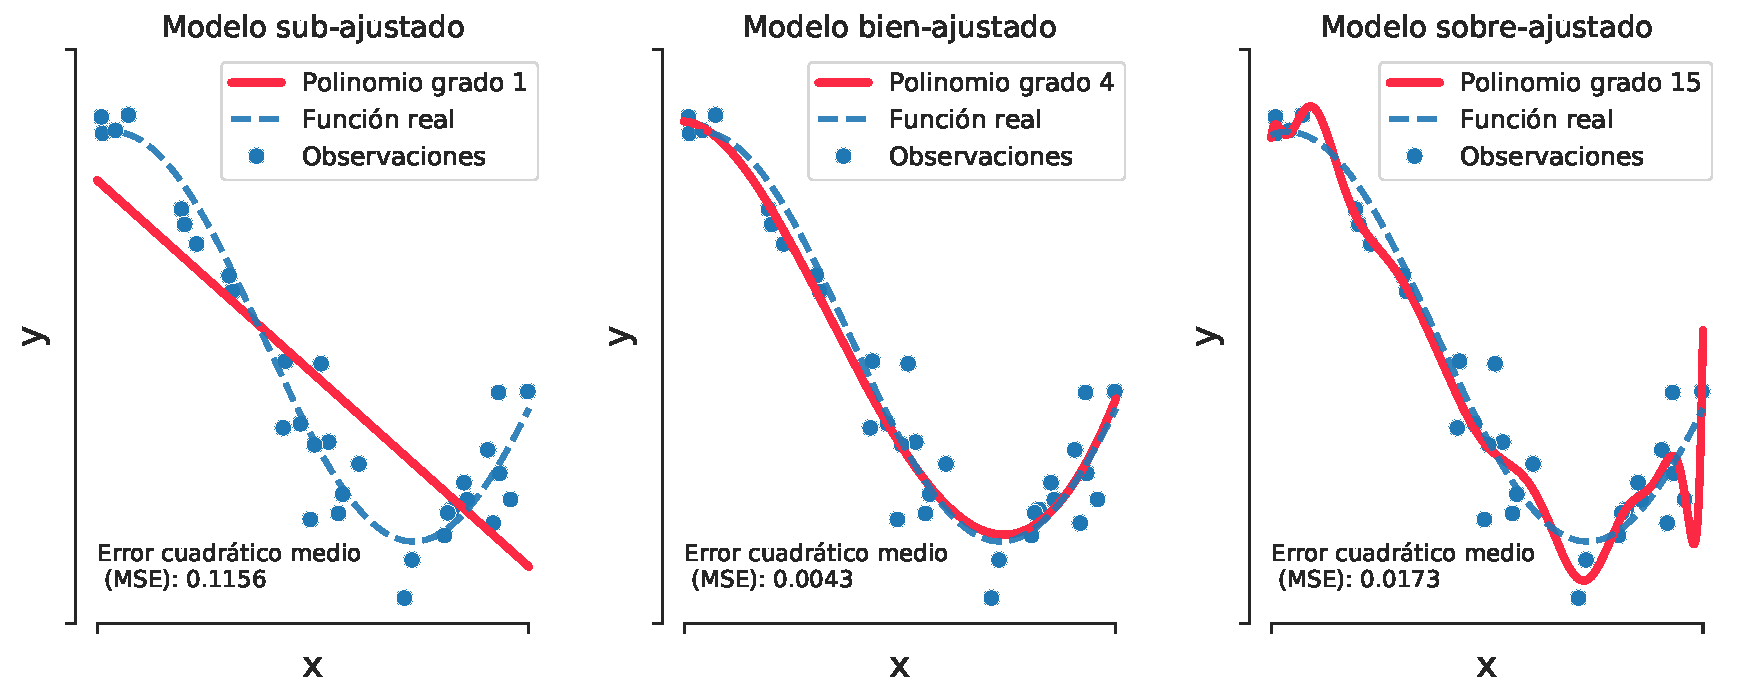
\includegraphics[width = 0.9\linewidth]{img/cap3_ajuste.pdf}
    \caption{Ejemplos de sub, sobre y correcto ajuste.}
    \label{fig:overfitting}
\end{figure}

La elección de modelo es uno de los problemas más recurrentes en análisis de datos, un ejemplo es la elección de las variables para la regresión ¿Por qué elegir un modelo cuadrático y no uno cúbico? ¿Por qué no incorporar todas las variables cruzadas ($X_1X_2, X_1X_3, ..., X_nX_m$)? Estas preguntas son fácilmente abordables si volvemos a la realidad y queremos correr los modelos en nuestros computadores: Incorporar más variables usualmente aumenta la complejidad computacional y con esto el tiempo de cómputo.

Bajo la filosofía anterior, encontrar un  \textit{trade-off} entre \emph{bias} (la flexibilidad del modelo de ajustarse a los datos) y performance sería lo ideal. Es por esta razón que crear un estadístico que pudiera expresar correctamente el compromiso precisión - flexibilidad ayudaría en la elección de modelo. Esto último es lo que busca relizar el \emph{Akaike Information Criterion} (AIC) y el \emph{Bayesian Information Criterion} (BIC) los cuales son dos enfoques distintos para abordar esta problemática.

\subsection{Criterio de Información Akaike}
La siguiente aproximación es válida cuando $N \to \infty$:

\begin{equation*}
-2\mathbb{E}[\log P_{\hat{\theta}}(Y)] \approx \frac{-2}{N}\mathbb{E}[\log L] + 2\frac{d}{N},
\end{equation*}

en donde $d$ es la cantidad de parámetros del modelo y  $L$ es la función de verosimilitud definida por:

\begin{equation}
L = \prod_{i=1}^N P(y_i|\hat{\theta}).
\end{equation}

De esta manera se define el estadístico AIC de la forma:

\begin{equation}
AIC(M) = 2d-2\log(L)
\end{equation}

Otros autores definen el estadístico como:

\begin{equation}
AIC(M) = 2\frac{d}{N}-2\frac{log(L)}{N}.
\end{equation}
Donde N es la cantidad de observaciones.

\textbf{\underline{Ejemplo:}} Si tenemos un conjunto de modelos $f_{\alpha}(x)$ indexados por un parámetro $\alpha$ de modo que el modelo $\alpha$ sigue un modelo gaussiano, es decir:
$$
\log(L) = -\sum_{i}(y_i-\hat{f}(x_i))^2/(2\sigma_e^2),
$$

\noindent entonces el estimador AIC se puede escribir como
\begin{equation}
\text{AIC}(M) = 2d(\alpha)-\overline{err}(\alpha),
\end{equation}
en donde la función $d(\alpha)$ denota una medida de la complejidad del modelo y $\overline{err}(\alpha)$ denota el error promedio del modelo $\alpha$.

\subsection{Criterio de Información Bayesiano}
Nuevamente, si nuestro setting nos permite obtener el máximo de la función de verosimilitud. Podemos utilizar el \emph{Bayesian Information Criterion} (BIC) el cual está definido por:

\begin{equation}
\text{BIC}(M) = log(N)d-2\log(L)
\end{equation}

En donde N es la cantidad de observaciones, $d$ es la cantidad de parámetros del modelo y L es el máximo de la función de verosimilitud. Este criterio también es conocido como \emph{Schwarz criterion}. Este estadístico se dice bayesiano por que se obtiene de realizar una aproximación de laplace sobre sobre $\log\mathbb{P}(X|M)$ obteniéndose:

\begin{equation}
\log\mathbb{P}(X|M) \approx \log\mathbb{P}(X|\hat{\theta}_m, M) - \frac{d_m}{2}(\log(N)-\log(2\pi))
\end{equation}

Donde $\hat{\theta}_m$ es el máximo del estimador de verosimilitud. Luego para $N$ muy grande se observa que la expresión $-2\log\mathbb{P}(X|M) = BIC(M)$.

\textbf{\underline{Ejemplo:}} Asumiendo que el modelo sigue un modelo gaussiano, es decir:
$$
\log(L) = -\sum_{i}(y_i-\hat{f}(x_i))^2/(2\sigma_e^2),
$$se tiene que el estadístico BIC está dado por:

\begin{equation}
BIC(M) = \frac{N\overline{err}(M)}{\sigma_e^2} + log(N)d
\end{equation}


\subsection{Evaluación y comparación de modelos}
Existen varias formas de evaluar un modelo, una de ella podría ser simplemente evaluar la precisión de sus predicciones. A veces fijarse es natural fijarse en la precisión, como en los problemas de pronóstico. Otras veces la precisión es importante para evaluar diferentes modelos y elegir uno de ellos. En esta sección presentaremos dos maneras distintas de evaluar modelos, cada forma sirve en distintos escenarios, los cuales se discutirán a través de la predicción puntal, que resume la predicción de un conjunto de datos en una solo valor.

\subsubsection{Error cuadrático medio}

El ajuste del modelo a nuevos datos se puede resumir en una predicción puntual llamada error cuadrático medio, el cual está definido por:

\begin{equation}
MSE(\theta) = \frac{1}{n}\sum_{i=1}^N (y_i-\mathbb{E}(y_i|\theta))^2
\end{equation}

o su versión ponderada:

\begin{equation}
MSE(\theta) = \frac{1}{n}\sum_{i=1}^N \frac{(y_i-\mathbb{E}(y_i|\theta))^2}{\mathbb{V}\text{ar}(y_i|\theta)}
\end{equation}

\subsubsection{log-densidad predictiva o log-verosimilitud}
Otra forma de realizar esta evaluación es utilizando el estadístico \emph{log-densidad preditiva} $\log p(y|\theta)$ el cual es proporcional a error cuadrático medio si el modelo es normal con varianza constante. Estudiaremos el caso de un solo punto, para luego extrapolar a más de un punto.

\textbf{Predictive accuracy para un punto}: Sea $f$ el modelo real, $y$ las observaciones (es decir, una realización del dataset $y$ de la distribución $f(y)$), y llamaremos $\tilde{y}$ a la data futura o un dataset alternativos que podemos ver. El ajuste predictivo out-of-sample para un nuevo punto $\tilde{y}_i$ está dado por:

\begin{equation}
\log p_{\text{post}}(\tilde{y}_i) = \log \mathbb{E}[p(\tilde{y}_i|\theta)] = \log \int p(\tilde{y}_i|\theta)p_{\text{post}}(\theta)d\theta
\end{equation}

\textbf{Promedio de las distribuciones para un punto}: Al tener un dato nuevo $\tilde{y}_i$ entonces se puede calcular el la log-densidad predictiva (elpd, por su sigla en inglés) para el nuevo punto:
\begin{align}
\notag \text{elpd} & = \mathbb{E}_f[\log p_{\text{post}}(\tilde{y}_i)]\\
& = \int \log p_{\text{post}}(\tilde{y}_i) f(\tilde{y}_i)d\tilde{y}
\end{align}

\textbf{Promedio de las distribuciones para datasets futuros}: Como usualmente, no se tiene solo un punto, se debe realizar la suma sobre el conjunto de puntos, calculando así la log-densidad predicitiva puntual (elppd, por su sigla en inglés).

\begin{align}
\text{elppd} & = \sum_{i=1}^N \mathbb{E}_f[\log p_{\text{post}}(\tilde{y}_i)]
\end{align}

En la práctica, como siempre se tiene la distribución de todos los modelos y la expresión anterior requiere de esto, se suele calcular el estadístico sobre una estimación de un modelo $\hat{\theta}$ (como por ejemplo, el máximo de la función de verosimilitud):

\begin{align}
\text{elppd}|\hat{\theta} & = \sum_{i=1}^N \mathbb{E}_f[\log p_{\text{post}}(\tilde{y}_i|\hat{\theta})]
\end{align}

Finalmente, una última extensión de este estadístico es cuando se puede tener \emph{draws} de la posterior, es decir, tenemos $\{ \theta^s\}_{s=1}^S$, entonces el lppd computado es:

\begin{equation}
\text{computed lppd} = \sum_{i=1}^N \left( \frac{1}{S} \sum_{s=1}^S p(y_i|\theta^s)\right)
\end{equation}

\subsubsection{Otros métodos}
Existen otros estadísticos o métodos que se pueden utilizar para comparar modelos. 

\begin{itemize}
    \item \textbf{Deviance Information Criterion:} Se podría decir que es una versión bayesiana de AIC, donde se realizan dos cambios principales 1) se cambia la estimación del estimador de máxima verosimilitud, por el promedio de la posterior y 2) se reemplaza k con una perrción de sesgo de los datos. Formalizando:
    
    \begin{equation}
        \text{DIC} = -2 \log(y|\hat{\theta}_{Bayes}) + 2p_{\text{DIC}},
    \end{equation}
    donde $p_{\text{DIC}}$ está dado por:
    
    \begin{equation}
        p_{\text{DIC}} = 2(\log(p(y|\hat{\theta}_{Bayes})- \mathbb{E}_{\text{post}}(\log(p(y|\theta)).
    \end{equation}
    
    Nuevamente, puede haber un versión \emph{computada} que está dada por:
    
    \begin{equation}
        \text{computed }p_{\text{DIC}} = 2[\log(p(y|\hat{\theta}_{Bayes})- \frac{1}{S}\sum_{s=1}^S \log (p(y|\theta^s))].
    \end{equation}
    %-------------------------------
    \item \textbf{Watanabe-Akaike o widely available information criterion:} WAIC es un forma aún más bayesiana para abordar el problema de asginación de evaluación. 
    
    \begin{equation}
        \text{WAIC} = -2 \text{lppd} + 2 p_{\text{WAIC}}
    \end{equation}
    
    donde hay dos formas de calcular $p_{\text{WAIC}}$.
    
    \begin{align}
    p_{\text{WAIC}1} &= 2 \sum_{i= 1}^n \left( \log(\mathbb{E}_{\text{post}}[p(y_i|\theta)]) - \mathbb{E}_{\text{post}}[\log (p(y_i|\theta))\right)\\
    p_{\text{WAIC}2} &= \sum_{i= 1}^n \left( \mathbb{V}\text{ar}_{\text{post}}[\log(p(y_i|\theta))]\right).
    \end{align}
    %-------------------------------    
    \item \textbf{Leave-one-out cross-validation:} También se puede usar validación cruzada bayesiana para estimar $-2\text{lppd} + 2\text{lppd}_{\text{loo-cv}}$ la cual sirve como estadístico de comparación:
    
    \begin{equation}
    \text{lppd}_{\text{loo-cv}} = \sum_{i=1}^n \log p_{\text{post}(-i)}(y_i)
    \end{equation}
    
    que se calcula como:
    
    \begin{equation}
    \text{computed lppd}_{\text{loo-cv}} = \sum_{i=1}^n \log \left( \sum_{s=1}^S \frac{1}{S} p(y_i|\theta^{is})\right)
    \end{equation}
    
    también se puede calcular a versión insesgada, la cual no se utiliza mucho pero se presenta por completitud:
    \begin{equation}
    \text{lppd}_{\text{cloo-cv}} = \text{lppd}_{\text{loo-cv}} + b.
    \end{equation}
    Donde $b$ está dado por:
    
    \begin{align}
    b = \text{lppd}_{-i} - \overline{\text{lppd}_{-i}},
    \end{align}
    
    con 
    
    \begin{align}
    \overline{\text{lppd}_{-i}} & = \frac{1}{n} \sum_{i=1}^n\sum_{j=1}^n \log p_{\text{post}(-i)}(y_j)\\
    \text{computed }\overline{\text{lppd}_{-i}} & = \frac{1}{n} \sum_{i=1}^n\sum_{j=1}^n \log \left( \frac{1}{S}\sum_{s=1}^S p(y_j|\theta^{is})\right).
    \end{align}
    
\end{itemize}

\subsection{Promedio de Modelos}
Hay veces que no queremos elegir solo un modelo, puesto que quizás nos interesan las estimaciones de dos o más modelos. Para estos casos, se puede utilizar la técnica de \emph{Model Averaging}, la cual consiste en simplemente ponderar los modelos de la siguiente forma:

\begin{equation}
\hat{\mu} = \sum_{s\in A} c(s) \hat{\mu}_s
\end{equation}
donde $A$ es el conjunto de todos los modelos. Además, se debe cumplir que:
\begin{equation}
\sum_{s\in A} c(s) = 1
\end{equation}

Notemos que la elección:

\begin{equation}
c(s) =
\begin{cases}
1 & \text{modelo con mejor criterio.}\\
0 & \sim
\end{cases}
\end{equation}

es una elección de pesos posible.

\subsubsection{Elección de pesos mediante softmax}

La principal dificultad para elegir los pesos, está en que se debe asegurar 1) la suma de los pesos sea unitaria, 2) que los pesos sean todos positivos. Una forma de asegurar esto es aplicar una función $f$ positiva sobre una función $g$ de \emph{score}, de modo que:

\begin{equation}
\sum_{s\in A} (f\circ g)(s) > 0
\end{equation}

Así los pesos quedan se pueden definir cómo:

\begin{equation}
c_f(s) = \frac{(f\circ g)(s)}{\sum_{z\in A} (f\circ g)(s)}
\end{equation}

La elección más común de para $f(x) = \text{softmax}(x)$, mientras que para la función de \emph{score} se puede utilizar las recién estudiadas AIC o BIC.

\begin{align}
c_{AIC}(s) = \frac{\exp\{ \frac{1}{2} \text{AIC}_s\}}{\sum_{z\in A} \exp\{ \frac{1}{2} \text{AIC}_z\}} & & c_{BIC}(s) = \frac{\exp\{ \frac{1}{2} \text{BIC}_s\}}{\sum_{z\in A} \exp\{ \frac{1}{2} \text{BIC}_z\}}
\end{align}


\subsubsection{Bayesian Model Averaring}

Supongamos que tenemos $\{M_j\}_{j=1}^k$ modelos, de los cuales todos realizan estimaciones razonables de una cantidad $\mu$, dado los datos $y$.
Para realizar el modelo promedio bayesiano de estos modelos es necesario encontrar la distribución posterior de $\mu$ dado los datos $y$ sin condicionar a un modelo en específico. De este modo, es necesari:
\begin{enumerate}
    \item Cada modelo tenga los mismos puntos de interpolación.
    \item Prior para cada modelo $p(M_j)$.
    \item Prior sobre los parámetros de los modelos $\pi(\theta_i|M_j)$\footnote{Se puede obtener mediante MCMC.}.
\end{enumerate}


Luego se puede calcular la función de verosimilitud para los parámetros:

\begin{equation}
\mathcal{L}_{\theta_j}(y) = p(y|\theta_j)
\end{equation}

Luego se marginaliza sobre los parámetros para obtener la función de verosimilitud del modelo:

\begin{align}
\lambda_{M_j}(y) & = p(y|M_j)\\
& = \int \mathcal{L}_{\theta_j}(y) \pi(\theta_i|M_j) d\theta_j\label{eq:lambda}
\end{align}

La expresión \eqref{eq:lambda} es también densidad marginal de las observaciones. Con esto la densidad posterior del modelo es:

\begin{align}
p(M_j|y) = \frac{p(M_j)\lambda_{M_j}(y)}{\sum_{l=1}^k p(M_{l})\lambda_{M_{l}}(y)}    
\end{align}

Finalmente, se puede obtener la distribución posterior para $\mu$ asumiendo que el modelo $M_j$ es verdadero ($\pi(\mu|M_j,y)$), y así, la distribución posterior buscada:

\begin{equation}
\pi(\mu|y) = \sum_{j = 1}^k p(M_j|y)\pi(\mu|M_j,y)
\end{equation}

\newpage
%!TEX root = notas_de_clase.tex

\newpage
\centerline{--------------------------------- clase X/4/18 ---------------------------------}
\section{Redes Neuronales - Editado}

\subsection{Introducci\'on y Arquitectura}

\subsubsection{Conceptos B\'asicos}

Los modelos escenciales de redes neuronales se conocen como \textbf{feedforward neural networks}, o \textbf{multilayer perceptrons} (MLPs). Una red neuronal busca aproximar una funci\'on $f^*$. Una red feedforward define un mapping $\bm{y}=f(\bm{x}; \bm{\theta})$ y aprende los par\'ametros $\bm{\theta}$ que resultan en la mejor aproximaci\'on posible.

Estos modelos se conocen como redes ya que que t\'ipicamente son el resultado de composiciones sucesivas de varios tipos de funciones. Por ejemplo, sean $f^{(1)}$, $f^{(2)}$ y $f^{(3)}$ funciones, estas se 'conectan' para formar $f(\bm{x}) = f^{(3)}(f^{(2)}(f^{(1)}(\bm{x})))$, se dice que $f^{(1)}$ es la primera \textbf{capa} de la red, $f^{(2)}$ la segunda y $f^{(3)}$ la tercera. El largo de esta cadena define la \textbf{profundidad} de la red. El uso de redes neuronales con m\'ultiples capas se conoce como \textbf{deep learning}, aunque este t\'ermino se usa para problemas m\'as espec\'ificos de aprendizaje de m\'aquinas usando redes neuronales profundas (ver secci\'on 3.5).

Durante el entrenamiento de una red neuronal se busca que $f(\bm{x}) \approx f^*(\bm{x})$, donde la data de entrenamiento provee aproximaciones ruidosas de $f^*(\bm{x})$. Cada dato $\bm{x}$ viene acompa{\~{n}}ado de una etiqueta, $y \approx f^*(\bm{x})$. Los datos de entrenamiento indica qu\'e debe reproducir la red en su \'ultima capa, lo cual debe ser un valor aproximado de $y$. El comportamiento del resto de las capas no tiene una interpretación tan directa como la última capa, por lo que el algoritmo de aprendizaje debe decidir c\'omo adaptar las capas para que el output producido por la red sea lo m\'as cercano posible a $y$, la etiqueta, para cada punto $\bm{x}$. Es por esto que estas capas intermedias se denominan \textbf{capas ocultas}.

Estas redes se llaman \textit{neuronales} por su inspiraci\'on neurocient\'ifica. Cada capa oculta de la red corresponde a un vector. Se podr\'ia pensar que cada elemento de estos vectores tiene un rol similar al de una neurona, en vez de pensar cada capa como una funci\'on que produce un mapping de vector a vector, podr\'ia considerarse que una capa consiste en muchas \textbf{unidades} que act\'uan en paralelo, cada una representando un mapping de vector a escalar. La elecci\'on de las funciones $f^{(i)}(\bm{x})$, conocidas como \textbf{funciones de activaci\'on}, en varios casos ha sido guiada por observaciones sobre el comportamiento de neuronas biol\'ogicas.

\begin{figure}[H]
\captionsetup{font=small,labelfont=small}
\caption{Ejemplo de una red neuronal de 1 capa: (\textit{izquierda}) Se muestra la red con inputs $x_1$ y $x_2$, que luego pasan a la capa oculta para producir el output $y$. (\textit{derecha}) Misma red con una representaci\'on vectorial de las capas. La matriz ${\bm{W}}$ describe el mapping de ${\bm{x}}$ a ${\bm{h}}$, y la matriz $w$ el mapping de ${\bm{h}}$ a $y$.}
\centering
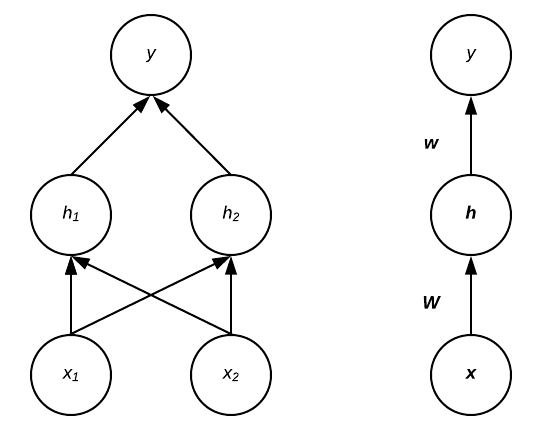
\includegraphics[scale=.5]{img/F1NN1L.png}
\end{figure}

Como se puede apreciar en la figura, los coeficientes ${\bm{W}}$ y $w$ se usan para producir el output para la siguiente capa (denominados \textbf{pesos}), por lo que la primera operaci\'on de esta red ser\'a entregar $h_{1}$ y $h_{2}$ mediante la transformaci\'on ${\bm{W}^{T}}\bm{x} + \bm{b}^{(1)}$. Luego, esta red aplica $w^{T} \boldsymbol{h} + b^{(2)}$ para producir el output $y$. Los coeficientes $\bm{b}^{(1)}$ y  $b^{(2)}$ se conocen como t\'erminos de \textbf{bias} (sesgo). Todos los parámetros de la red neuronal, los pesos y \textit{bias}, serán agrupados en el t\'ermino $\bm{\theta}$.

\subsubsection{Funci\'on de Costos, Unidades de Output y la Formulaci\'on como un Problema Probabil\'istico}

Una de las principales diferencias entre los modelos lineales antes vistos y una red neuronal, es que el uso de ciertas funciones de activaci\'on hacen que la funci\'on de costos no sea convexa, esto hace que el entrenamiento realizado en base a descenso de gradiente no entregue garant\'ias de que se alcanzar\'a el \'optimo global, o una buena solución en términos generales, ya que el algoritmo podría estancarse en un optimo local que entregue resultados pobres. 

En la mayor\'ia de los casos, el modelo param\'etrico define una distribuci\'on $p(y|\bm{x}; \bm{\theta})$, por lo que los par\'ametros del modelo se estimar\'an usando m\'axima verosimilitud, as\'i, se optimizar\'a la log-verosimilitud negativa, es decir, la \textbf{funci\'on de costos} a usar ser\'a la \textbf{cross-entropy}:

\begin{equation}
J(\bm{\theta}) = -\E_{\bm{x},\bm{y}\sim \hat{p}_{\textrm{data}}}(\textrm{log}\; p_{\textrm{modelo}}(\bm{y}|\bm{x}))
\end{equation}

De esta forma la elecci\'on de la \textbf{unidad de output} definir\'a la forma que toma la funci\'on de costos, pero no ser\'a necesario definir una funci\'on especifica para cada problema; en general siempre se resolver\'a el problema por m\'axima verosimilitud. La elecci\'on en la unidad de output depender\'a del tipo de problema que se quiera resolver. Cuando se quiera retornar la media de una distribuci\'on Gaussiana condicional, $p(\bm{y}|\bm{x}) = \mathcal{N}(\bm{y}|\hat{\bm{y}};\bm{I})$, la unidad de output deber\'a ser un modelo lineal, $\hat{\bm{y}} = \bm{W}^{T}\bm{h} + \bm{b}$, en donde $\bm{h}$ es el output de la red que proviene de todas las capas ocultas anteriores. En este caso, maximizar la log-verosimilitud es equivalente a minimizar el error cuadr\'atico medio, por esta razón este tipo de output es adecuada para un problema de regresión.

Cuando el problema objetivo es clasificaci\'on binaria, una unidad de output apropiada es la funci\'on sigmoidal. Para resolver el problema de m\'axima verosimilitud, se modela utilizando una distribuci\'on Bernoulli en $y$ condicional en $\bm{x}$. Una unidad de output sigmoidal se define como $\hat{{y}} = \sigma(\bm{w}^{T}\bm{h} + {b})$. Esto entrega como output $P(y=1|\bm{x})$, por lo que se podr\'a decidir a qu\'e clase pertenece $y$ basado en el output de la red, esto se interpreta como la probabilidad de que la observaci\'on sea de la clase 1.

Para un problema de clasificaci\'on multiclase, la unidad de output apropiada es la generalizaci\'on de la funci\'on sigmoidal, conocida como softmax. El problema es predecir a cu\'al de $n$ clases pertenece $y$, por lo que se requiere producir un vector $\hat{\bm{y}}$, con $\hat{y_{i}} = P(y=i|\bm{x})$, por lo que se usar\'a una distribuci\'on multinoulli. Primero, una capa lineal predice las log-probabilidades no normalizadas, $\bm{z} = \bm{W}^{T}\bm{h} + \bm{b}$, y luego se aplica la funci\'on softmax para obtener los valores de $\hat{\bm{y}}$ antes descritos:

\begin{equation}
\textrm{log softmax}(\bm{z})_{i} = \textrm{log}\frac{\textrm{exp}(z_{i})}{\sum_{j=1}^{n}\textrm{exp}({z_{j}})} = z_{i} - \textrm{log}\sum_{j=1}^{n}\textrm{exp}({z_{j}})
\end{equation}

\subsubsection{Estructura Interna de la Red}

Las capas escondidas proveen a la red neuronal la flexibilidad necesaria para aprender funciones extremadamente complejas, esto mediante el uso de activaciones no lineales. En varios casos estas funciones son incluso no diferenciables, lo que llevar\'ia a pensar de que no son v\'alidas para ser usadas en conjunto con algoritmos que usan descenso de gradiente, pero en la pr\'actica tienen un desempe\~{n}o suficientemente bueno para ser usadas en tareas de aprendizaje de m\'aquinas. En general, las funciones de activaci\'on para las unidades escondidas toman como input un vector $\bm{x}$ para el cual obtienen una transformaci\'on af\'in $\bm{z} = \bm{W}^{T}\bm{x} + \bm{b}$, para luego aplicar una transformaci\'on no lineal $g(\bm{z})$. Las unidades escondidas m\'as comunes son las \textbf{rectified linear units} o \textbf{ReLUs}, $g(\bm{z}) = \textrm{max}(0, \bm{z})$, y sus generalizaciones como \textbf{leaky ReLU}, $g(\bm{z})_{i} = \textrm{max}(0, \bm{z}_{i}) + \alpha_{i}\textrm{min}(0, \bm{z}_{i})$, con $\alpha_{i}$ una constante peque\~{n}a como 0.01; la funci\'on sigmoidal $g(\bm{z}) = \sigma(\bm{z})$; y la tangente hiperb\'olica $g(\bm{z}) =  \textrm{tanh}(\bm{z}) = 2\sigma(2\bm{z}) - 1$. A diferencia de las funciones lineales por partes, las unidades sigmoidales se saturan en la mayor parte de su dominio (su gradiente se aproxima a 0) haciendo imposible el aprendizaje por el gradiente cuando esto ocurre, por lo que su uso como unidades escondidas ha sido desalentado.

\subsubsection{Dise\~{n}o de Arquitectura y Teorema de Aproximaci\'on Universal}

La \textbf{arquitectura} de una red neuronal se refiere a la totalidad de su estructura: la cantidad de capas, la cantidad de unidades escondidas, la conexi\'on entre las unidades, etc. Bajo la estructura mostrada para una red feedforward, la primera capa y la segunda capa son de la forma:

\begin{equation}
\begin{split}
\bm{h}^{(1)} = g^{(1)}(\bm{W}^{(1) T}\bm{x} + \bm{b}^{(1)}) 
\\
\bm{h}^{(2)} = g^{(1)}(\bm{W}^{(2) T}\bm{h}^{(1)} + \bm{b}^{(2)})
\end{split}
\end{equation}

En una arquitectura de este tipo, la principal consideraci\'on respecto al dise\~{n}o es la profundidad y ancho (cantidad de unidades por capa) de cada capa. Una red con solo 1 capa escondida puede ser suficiente para ajustar el set de entrenamiento, cabe destacar que la cantidad de neuronas necesarias en esta única capa podría ser muy grande y la capacidad de generalización puede ser baja, dependiendo de la complejidad de los datos con los que se pretende trabajar. Redes m\'as profundas generalmente permiten disminuir el n\'umero de unidades por capa (de esta forma tener una menor cantidad par\'ametros en total), como as\'i tambi\'en una mejor capacidad de generalización en el set de testeo, con esto se hace referencia a la capacidad de la red para clasificar correctamente ejemplos que no fueron usados para el proceso de entrenamiento, naturalmente hacer más intrincado el diseño de la red hará que el proceso de optimización para ajustar los parámetros sea más costoso. La arquitectura ideal se debe encontrar por experimentaci\'on con distintas estructuras acompañado de conocimiento sobre el tipo de datos, esto se apoya mediante el monitoreo del error en el set de validaci\'on.

Una de las principales justificaciones para usar redes neuronales se debe al \textbf{Teorema de Aproximaci\'on Universal} (Horniket al., 1989; Cybenko, 1989), el cual muestra que una red feedforward con una capa de output lineal y al menos una capa escondida con funci\'on de activaci\'on sigmoidal (y otras similares) puede aproximar cualquier funci\'on Borel medible \footnote{En particular cualquier funci\'on continua en un subconjunto cerrado y acotado de $\R^{n}$ es Borel medible, la clase de funciones Borel medibles es mucho más rica y variada que las funciones continuas.} de un espacio dimensión finita a otro, con un nivel de error arbitrariamente pequeño, provisto de que hayan suficientes unidades escondidas. Una red neuronal tambi\'en puede aproximar un mapping de cualquier espacio dimensional finito y discreto a otro, y este teorema tambi\'en se ha probado para una amplia gama de funciones de activaci\'on, como para la m\'as com\'unmente usada ReLU (Leshno et al., 1993). La desventaja del teorema es que a pesar que asegura que la red podr\'a aproximar cualquiera de estas funciones, esto no implica que necesariamente podr\'a \textit{aprender} la funci\'on en sí. Una razón posible es que el algoritmo de optimizaci\'on podr\'ia no encontrar los par\'ametros de la red que alcancen el nivel de error deseado. Tampoco especifica la cantidad de unidades que son necesarias para alcanzar un nivel de error dado, lo cual podr\'ia ser excesivamente grande. Sin embargo en muchos casos modelos m\'as profundos necesitar\'an menos unidades y potencialmente permiten reducir el error de generalizaci\'on.

\subsection{Entrenamiento de una Red Neuronal}

\subsubsection{Forward Propagation y Back-Propagation}

Al usar una red neuronal feedforward, la informaci\'on fluye a trav\'es de la red desde el ingreso de un input $\bm{x}$ hasta producir un output $\hat{\bm{y}}$. Esto se conoce como \textbf{forward propagation}. Durante el entrenamiento, \textit{forward propagation} contin\'ua hasta producir el costo escalar $J(\bm{\theta})$.

El algoritmo de \textbf{back-propagation} permite que la informaci\'on del costo fluya en sentido inverso a trav\'es de la red para calcular el gradiente de manera computacionalmente eficiente. El gradiente se calculará de esta forma ya que, aunque es posible obtener una expresi\'on anal\'itica para este, evaluar la expresi\'on puede ser muy caro computacionalmente. Luego de obtener el gradiente, otro algoritmo como descenso de gradiente estoc\'astico (ver secci\'on 4) realiza el aprendizaje usando la expresión que fue calculada. En algoritmos de aprendizaje el gradiente que m\'as com\'unmente se requiere obtener es $\nabla_{\bm{\theta}}J(\bm{\theta})$, aunque el algoritmo de \textit{back-propagation} no se limita a esto y puede ser usando para otras tareas que involucren obtener derivadas.

Sea $\bm{x} \in \R^{m}, \bm{y} \in \R^{n}, g:\R^{m} \rightarrow \R^{n}, f:\R^{n} \rightarrow \R, \bm{y} = g(\bm{x})$ y $z = f(\bm{y})$, la regla de la cadena indica que:

\begin{equation}
\frac{\partial z}{\partial x_{i}} = \sum_{j}\frac{\partial z}{\partial y_{j}}\frac{\partial y_{j}}{\partial x_{i}}
\end{equation}

O de manera equivalente visto en su forma vectorial:

\begin{equation}
\nabla_{\bm{x}}z = (\frac{\partial \bm{y}}{\partial \bm{x}})^{T}\nabla_{\bm{y}}z
\end{equation}

en donde $\frac{\partial \bm{y}}{\partial \bm{x}}$ es la matriz Jacobiana de $g$, con esto se puede ver que para obtener el gradiente con respecto a la variable $\bm{x}$, basta multiplicar la matriz Jacobiana por el gradiente con respecto a $\bm{y}$.% El algoritmo de \textit{back-propagation} consiste en realizar este tipo de operaciones iterativamente, calculando la regla de la cadena con un orden espec\'ifico de operaciones que lo hace altamente eficiente.


Usualmente se aplicar\'a \textit{back-propagation} a \textbf{tensores} de dimensionalidad arbitraria, no solo vectores. Se denota entonces el gradiente de $z$ con respecto a un tensor $\textrm{\textbf{X}}$ como $\nabla_{\textrm{\textbf{X}}}z$. Sean $\textrm{\textbf{Y}} = g(\textrm{\textbf{X}})$ y $z = f(\textrm{\textbf{Y}})$, entonces la regla de la cadena se escribe como:

\begin{equation}
\nabla_{\textrm{\textbf{X}}}z = \sum_{j}(\nabla_{\textrm{\textbf{X}}}\textrm{Y}_{j})\frac{\partial z}{\partial \textrm{Y}_{j}}
\end{equation}

%\newpage
%[AGREGAR DESCRIPCIÓN DE BACK-PROPAGATION]

Antes de proseguir a revisar los algoritmos de \textit{forward-propagation} y \textit{back-propagation} se realizará una breve deducción de \textit{back-propagation} que permitirá comprender de mejor manera el proceso de entrenamiento en una red neuronal, en primer lugar de analizará una red neuronal con solo una capa escondida, luego veremos que esto puede ser extendido de forma fácil a arquitecturas más complejas (osea, más capas).

Sea $\{ (x_i,y_i) \}_{i=1}^N$ un conjunto de puntos sobre los que se quiere ajustar los pesos de una red neuronal, el conjunto de entrenamiento es tal que  $x_i \in \R^p, y_i \in \R^K \quad \forall i=1,...,N$, el problema planteado corresponde a uno de clasificación sobre $K$ clases distintas. Adicionalmente se tiene que el error (función de perdida) puede ser escrito como:

\begin{equation}
J(\theta) = \sum_{i=1}^N J_i = \sum_{i=1}^N L(y_i, f(x_i;\theta))
\end{equation}

Donde $J_i$ corresponde a la discrepancia entre $y_i$ y el valor entregado por la red $f(x_i;\theta)$ evaluado por la función de perdida $L$. Para fijar ideas, la arquitectura de la red está compuesta por $p$ unidades de entrada, la capa escondida tiene $M$ neuronas con funciones de activación sigmoides ($\sigma(x)=\frac{1}{1-e^{-t}}$) y la capa de salida (output) tendrá $K$ unidades y una función de salida $g$. De esta forma el problema puede ser planteado como:

\begin{align}
	Z_m &= \sigma(\alpha_{0m} + \alpha_{m}^TX), \quad \forall m=1,...,M\\
	N_k &= \beta_{0k} + \beta_k^TZ, \quad\quad\quad \forall k=1,...,K\\
	O_k &= g_k(N), \quad\quad\quad\quad \forall k=1,...,K\\
	f(X) &= O\\
\end{align}

Donde $Z=(Z_1,...,Z_M)$, $N=(N_1,...,N_K)$, $O=(O_1,...,O_K)$ y se puede ver que $g:\R^K \rightarrow \R^K$, de esta forma los parámetros $\theta$ del modelo son:

\begin{align*}
\{\alpha_{0m}, \alpha_m; \quad m &= 1,...,M \} \quad M(p+1) \quad \text{pesos}\\
\{\beta_{0k}, \beta_k; \quad k &= 1,...,K \} \quad K(M+1) \quad \text{pesos}\\
\end{align*}

De ahora en adelante $J\equiv J(\theta)$, también es importante distinguir que es distinto calcular la derivada de $J$ respecto a un peso que está en la capa de salida y un peso que pertenece a una capa escondida, siendo el primer caso mucho más fácil de calcular, esto se justifica por el hecho que los valores de la capa de salida participan directamente en el calculo del error $J$, mientras que los valores de las neuronas escondidas no, esto se hará evidente en los cálculos. Como último preámbulo se definen las siguientes variables que nos ayudaran a hacer los cálculos más claros:

\begin{align*}
z_{mi} &= \sigma(\alpha_{0m} + \alpha_{m}^Tx_i)\\
z_i &= (z_{1i},...,z_{Mi})\\
n_{ki} &= \beta_{0k} + \beta_k^Tz_i\\
n_i &= (n_{1i},...,n_{Ki})\\
o_{i} &= g(n_i)\\
o_{ki} &= (o_i)_k\\
\end{align*}

Considerando que derivar es una operación lineal calcularemos la derivada de $J_i$, a partir de este termino podemos obtener la derivada de $J$ sumando sobre todo $i=1,...,N$.

\begin{align}
\frac{\partial J_i}{\partial \beta_{km}}&=
\frac{\partial J_i}{\partial o_{ki}}
\frac{\partial o_{ki}}{\partial n_{ki}}
\frac{\partial n_{ki}}{\partial \beta_{km}}\\
&= \frac{\partial J_i}{\partial o_{ki}}
g'_k(n_{ki})z_{mi}
\label{BP_beta}
\end{align}

Dado que $o_{ki}$ pertenece a la capa de salida, esto implica que participa directamente en la expresión de $J_i$ y por lo tanto la derivada $\frac{\partial J_i}{\partial o_{ki}}$ puede ser calculada directamente. El calculo recién hecho se conoce como regla delta ('delta rule') y es el paso principal de \textit{back-propagation}, este consiste en usar la regla de la cadena 2 veces sucesivamente.

Como se mencionó con anterioridad calcular la derivada de $J_i$ respecto a un peso perteneciente a una capa escondida es más engorroso, ya que las neuronas en las capas intermedias no participan directamente en el error, aún así es posible y el calculo entrega una formula recursiva que permite llegar a una expresión cerrada y explicita.

\begin{align}
\frac{\partial J_i}{\partial \alpha_{ml}}&=
\frac{\partial J_i}{\partial z_{mi}}
\frac{\partial z_{mi}}{\partial \alpha_{ml}}\\
&= \left [ \sum_{k=1}^K
\frac{\partial J_i}{\partial o_{ki}}
\frac{\partial o_{ki}}{\partial n_{ki}}
\frac{\partial n_{ki}}{\partial z_{mi}}
\right ]
\frac{\partial z_{mi}}{\partial \alpha_{ml}}\\
&= \left [ \sum_{k=1}^K
\frac{\partial J_i}{\partial o_{ki}}
\frac{\partial o_{ki}}{\partial n_{ki}}
\frac{\partial n_{ki}}{\partial z_{mi}}
\right ]\sigma'(\alpha_0+\alpha_mx_i)x_{il}\\
&= \left [ \sum_{k=1}^K
\frac{\partial J_i}{\partial o_{ki}}
g'(n_{ki})
\beta_{km}
\right ]\sigma'(\alpha_0+\alpha_mx_i)x_{il}\\
&=  \sum_{k=1}^K
\frac{\partial J_i}{\partial o_{ki}}
g'(n_{ki})
\beta_{km}
\sigma'(\alpha_0+\alpha_mx_i)x_{il}
\label{BP_alfa}
\end{align}

Al llegar a la expresión final se puede ver que todos los términos pueden ser calculados de forma explicita, en este punto se puede apreciar porqué el nombre \textit{back-propagation}, a partir de los cálculos obtenidos en las capas exteriores se pueden obtener derivadas de los pesos en capas anteriores, en este sentido la información se propaga 'hacia atrás' en la red. Finalmente reescribimos (\ref{BP_beta}) y (\ref{BP_alfa}) como:

\begin{equation}
	\frac{\partial J_i}{\partial \beta_{km}} = \delta_{ki}z_{mi}
	\quad\quad
	\frac{\partial J_i}{\partial \alpha_{ml}} = s_{mi}x_{il}
\end{equation}

Donde:

\begin{align}
\delta_{ki} &= 
\frac{\partial J_i}{\partial o_{ki}}
g'_k(n_{ki})\\
s_{mi} &= 
\sigma'(\alpha_0+\alpha_mx_i)\sum_{k=1}^K\beta_{km}\delta_{ki}
\end{align}

Las cantidades $\delta_{ki}$ y $s_{mi}$ son errores del modelo en la capa de salida y capas escondidas respectivamente, las 4 ultimas ecuaciones presentadas son conocidas como como ecuaciones de \textit{back-propagation}. Para extender el desarrollo a una red neuronal con más capas es importante notar que a partir de la capa final y la anterior se logró calcular todas las derivadas del gradiente del error, si se considerará la capa de entrada (input) como otra capa escondida más, se pueden repetir los mismos razonamientos y extenderlos a un nivel de profundidad arbitrario. 

%\newpage
A continuaci\'on se presentan los algoritmos de \textit{forward propagation} y \textit{back-propagation} para una red MLP en donde se conectan todas las unidades de una capa con la siguiente (fully connected MLP).

\begin{algorithm}[H] % H = forzar está posición 
\caption{Forward Propagation}\label{ML:Algorithm1}
\textbf{Requerir}: Profundidad de la red, $l$ \\
\textbf{Requerir}: $\bm{W}^{(i)}, i \in \{1,...,l\}$, pesos de la red \\
\textbf{Requerir}: $\bm{b}^{(i)}, i \in \{1,...,l\}$, parámetros bias de la red \\
\textbf{Requerir}: $\bm{x}$, el input \\
\textbf{Requerir}: $\bm{y}$, el output target \\
$\;\;\bm{h}^{(0)} = \bm{x}$\\
$\;\; \textrm{for} \;k = 1,...,l$:\\
$\;\;\;\;\;\;\bm{a}^{(k)} = \bm{b}^{(k)} + \bm{W}^{(k)}\bm{h}^{(k-1)}$\\
$\;\;\;\;\;\;\bm{h}^{(k)} = f(\bm{a}^{(k)})$\\
$\;\;\bm{\hat{y}} = \bm{h}^{(l)}$\\
$\;\;J = L(\bm{\hat{y}},\bm{y})$
\end{algorithm}

\begin{algorithm}[H] % H = forzar está posición
\caption{Back-Propagation}\label{ML:Algorithm2}
Luego de completar forward propagation: \\
$\bm{g} \leftarrow \nabla_{\bm{\hat{y}}} J = \nabla_{\bm{\hat{y}}} L(\bm{\hat{y}},\bm{y})$\\
$\textrm{for} \;k = l,l-1,...,1:$\\
$\;\;\;\;\nabla_{\bm{a}^{(k)}} J = \bm{g}\odot f'(\bm{a}^{(k)})$\\
$\;\;\;\;\nabla_{\bm{b}^{(k)}} J = \bm{g}$\\
$\;\;\;\;\nabla_{\bm{W}^{(k)}} J = \bm{g}\bm{h}^{(k-1)T}$\\
$\;\;\;\;\bm{g} \leftarrow \nabla_{\bm{h}^{(k-1)}} J = \bm{W}^{(k)T}\bm{g}$
\end{algorithm}

Con este algoritmo se obtienen los gradientes con respecto a todos los par\'ametros hasta la primera capa, propagando el gradiente desde una capa a la anterior mediante la \'ultima actualizaci\'on del algoritmo para cada iteraci\'on.

\subsection{Regularizaci\'on para una Red Neuronal}

Las redes neuronales y algoritmos de deep learning son aplicados a tareas extremadamente complejas como lo son el procesamiento de im\'agenes, audio, y texto. Controlar la complejidad de un modelo no solo se reduce a encontrar el tamaño y cantidad de parámetros adecuados, como se ha visto para otros modelos de aprendizaje de m\'aquinas, sino que en la pr\'actica el modelo con el mejor ajuste por lo general ser\'a un modelo grande (profundo) que ha sido regularizado apropiadamente.%El rol que juega la regularizaci\'on en un escenario como este no es solo controlar la complejidad del modelo buscando un modelo con tama{\~{n}}o  adecuado con el correcto n\'umero de par\'ametros, como se ha visto para otros modelos de aprendizaje de m\'aquinas, si no que en la pr\'actica el modelo con el mejor ajuste ser\'a un modelo grande (profundo) que ha sido regularizado apropiadamente.

\subsubsection{Regularizaci\'on $\bm{L}^{2}$}

Una regularizaci\'on que se basa en limitar la norma de los parámetros del modelo es la ya conocida \textbf{regularizaci\'on} $\bm{L}^{2}$ (o \textbf{ridge regression}), mediante la cual se obtiene la funci\'on objetivo regularizada $\tilde{J}$:

\begin{equation}
\tilde{J}(\bm{\theta};\bm{X},\bm{y}) = J(\bm{\theta};\bm{X},\bm{y}) + \frac{\alpha}{2}||\bm{\theta}||^{2}_{2}
\end{equation}

en donde el hiperpar\'ametro $\alpha \in [0,\infty[\ $ indica que tanta importancia se le da al termino de regularización sobre el objetivo, no habrá regularizaci\'on cuando $\alpha = 0$ y se observará un mayor efecto regularizador a medida que $\alpha$ crece. Cabe destacar que t\'ipicamente en una regularizaci\'on por la norma solo se regularizan los \textit{pesos}, dejando los t\'erminos de \textit{bias} sin regularizar. Esto ya que cada t\'ermino de \textit{bias} controla el comportamiento de solo 1 variable implicando que no se introduce mucha varianza \textbf{[(\textit{overfitting}), no se si es pertinente esta acotación]*} al dejarlos sin regularizar, por otro lado regularizar los \textit{bias} puede inducir un alto nivel de \textit{underfitting}.

\subsubsection{Dropout}

\textbf{Bagging} consiste en entrenar m\'ultiples modelos y evaluarlos en cada dato del set de testeo. Esto no es pr\'actico para redes neuronales\textbf{[Duda, según lo que vi baggin se refiera a cuando se entrenan muchos clasificadores y luego votan sobre el resultado]*}, ya que un solo modelo puede ser muy caro de entrenar y evaluar. \textbf{Dropout} provee una aproximaci\'on barata (computacionalmente) para entrenar y evaluar \textit{bagged} ensambles compuestos por una cantidad exponencial de redes neuronales. Dropout entrena los ensambles de posiblemente todas las subredes que se puedan formar al remover unidades (que no sean las de output) de un modelo de red neuronal (ver figura). Esto se puede realizar al multiplicar por 0 el output de alguna unidad para la mayor\'ia de los casos. Espec\'ificamente, para entrenar con dropout se usa un algoritmo por mini-batches (ver secci\'on 4) para que en cada iteraci\'on se entrene una subred aplicando una m\'ascara binaria a todas las capas de input y escondidas. Los hiperpar\'ametros de este m\'etodo de regularizaci\'on corresponden al dise{\~{n}}o de la m\'ascara binaria, especificando la probabilidad de que se incluya una unidad de input y la probabilidad de que se incluya una unidad escondida. T\'ipicamente se usan los valores 0.8 y 0.5, respectivamente, sin embargo estos deben ser ajustados para controlar el nivel de regularizaci\'on (mayor valor para las probabilidades implica menor efecto regularizador) para obtener un desempe{\~{n}}o \'optimo en el set de validaci\'on.

\begin{figure}[H]
\captionsetup{font=small,labelfont=small}
\caption{Dropout entrena potencialemente todas las subredes que se puedan formar a partir de la red neuronal original (primer recuadro) al apagar el output que producen las distintas unidades}
\centering
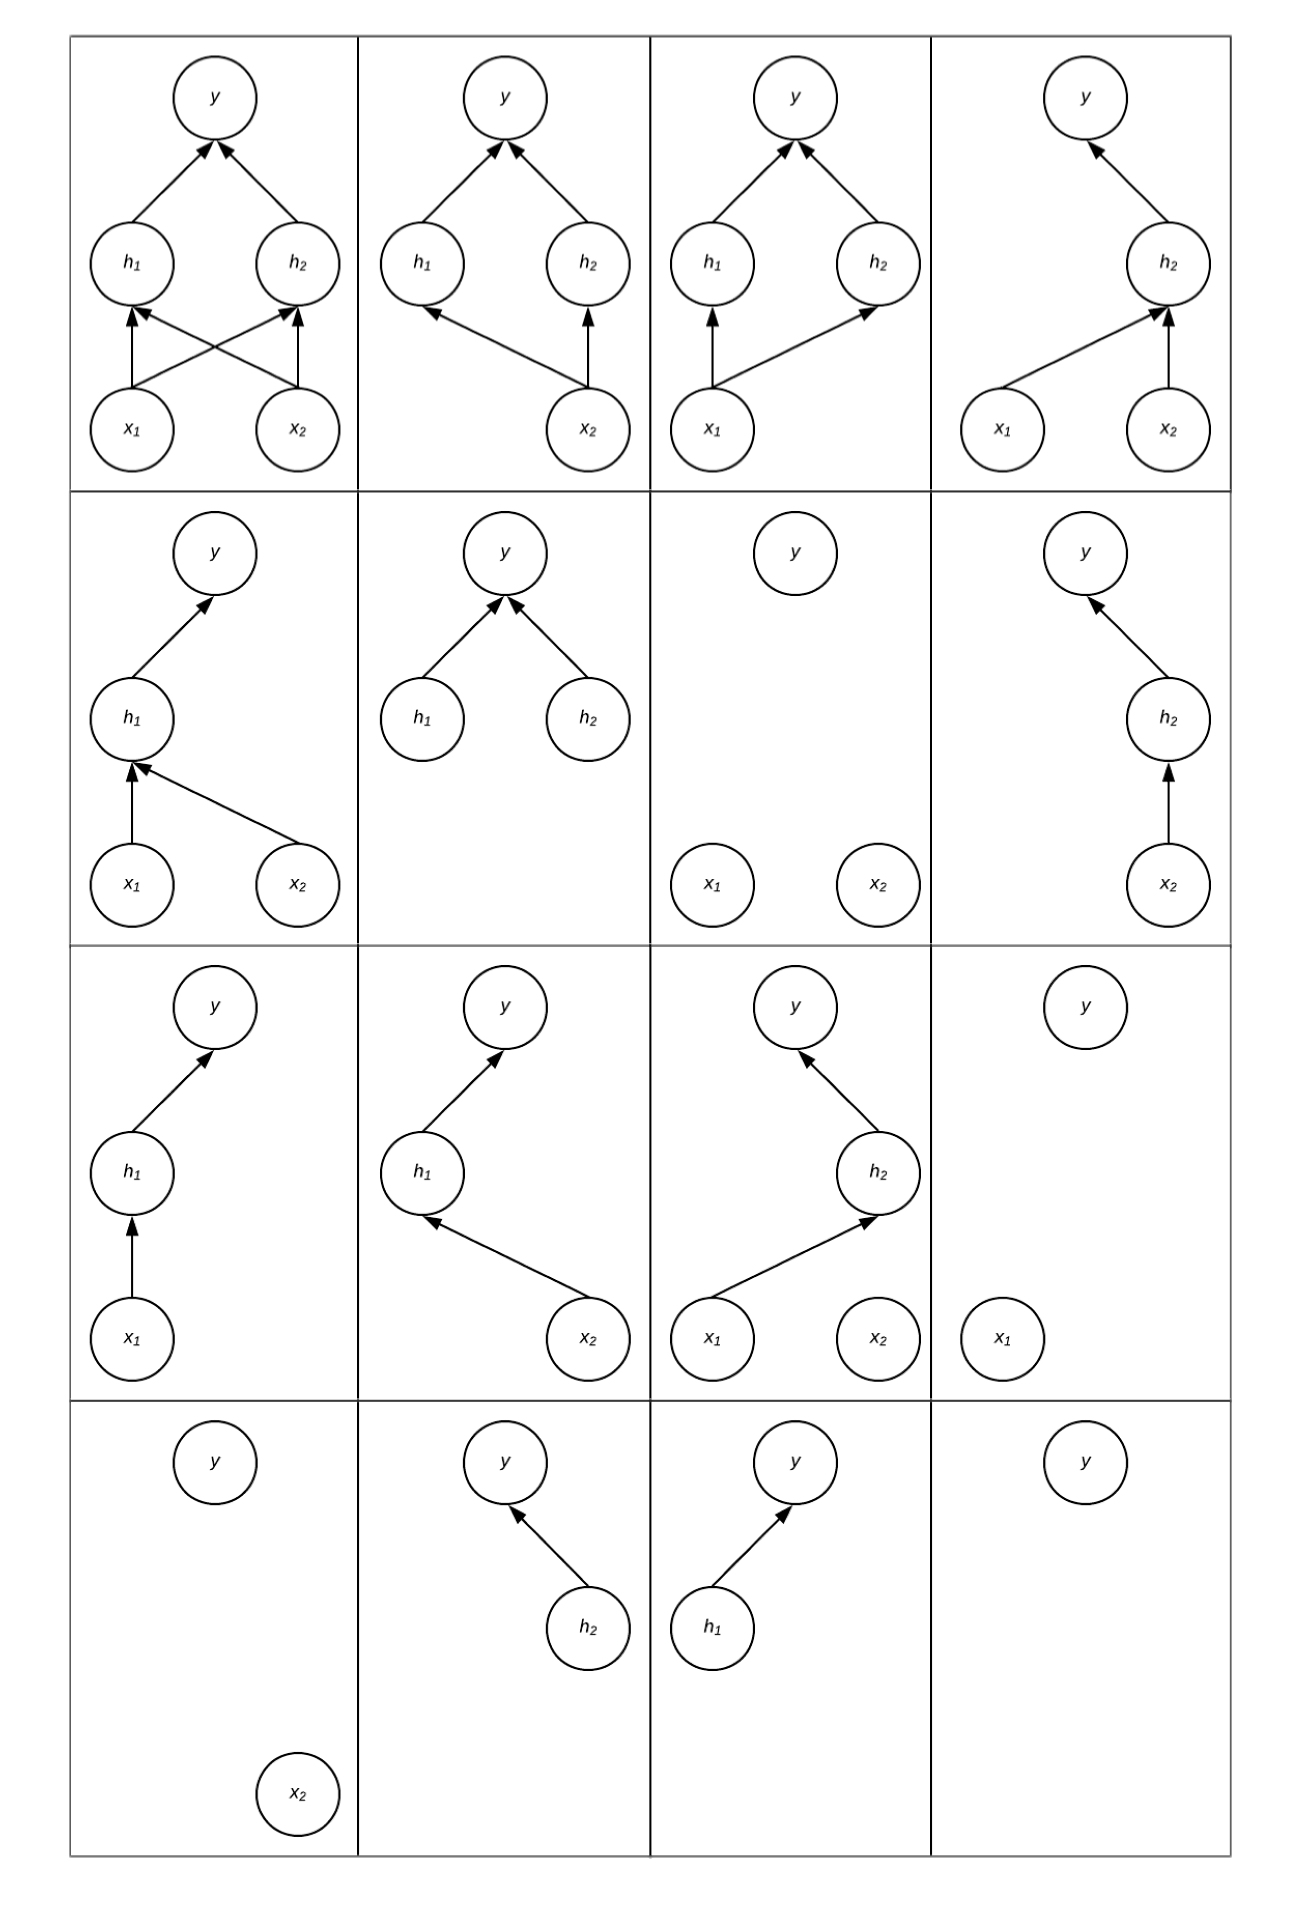
\includegraphics[scale=.25]{img/Dropout.png}
\end{figure}

\subsubsection{Otros M\'etodos de Regularizaci\'on}
Otras formas de regularizaci\'on tambi\'en buscan introducir alguna fuente de ruido (como en dropout) para que la red neuronal aprenda principalmente los par\'ametros m\'as importantes, as\'i logrando un bajo error de generalizaci\'on. Una de estas t\'ecnicas es \textbf{dataset augmentation}, que consiste en generar nuevos datos de entrenamiento (inyectando ruido en el set de entrenamiento), creando datos $\bm{x}$ falsos para los cuales se pueda tener una etiqueta $y$ (por ejemplo, una imagen invertida de un gato sigue siendo un gato), o \textbf{entrenamiento adversarial}, en donde se perturban ejemplos para fortalecer a la red (por ejemplo, cambiar pixeles de una imagen que generen cambios imperceptibles para un humano pero que pueden afectar fuertemente la capacidad de predicci\'on de un modelo). Otra t\'ecnica es \textbf{noise injection} en los pesos (Jim et al., 1996; Graves, 2011), lo cual se puede interpretar como una implementaci\'on estoc\'astica de inferencia Bayesiana sobre los pesos, debido a que el aprendizaje considerar\'ia que los pesos son inciertos y, por lo tanto, representables mediante una distribuci\'on de probabilidad.

Tambi\'en, por supuesto, \textbf{early stopping} es una t\'ecnica v\'alida para regularizar redes neuronales.

\subsection{Algoritmos de Optimizaci\'on}

Como ya se ha comentado, la optimizaci\'on en redes neuronales busca resolver un problema particular: encontrar los par\'ametros $\bm{\theta}$ que disminuyan significativamente $J(\bm{\theta})$, que depende de alguna medida de desempe{\~{n}}o evaluada en la totalidad del set de entrenamiento, luego se evaluá el error en el set de validaci\'on para tener una idea del desempeño, finalmente se ven los resultados en el set de testeo. 

Esto se reduce a minimizar la esperanza del error sobre la distribuci\'on generadora de los datos, $p_{\textrm{data}}$:

%[ posiblemente minimizando mediante hiperpar\'ametros tambi\'en una funci\'on de costos regularizada $\tilde{J}(\bm{\theta})$ ]

\begin{equation}
J^{*}(\bm{\theta}) = \E_{(\bm{x},y)\sim {p}_{\textrm{data}}}L(f(\bm{x};\bm{\theta}),y)
\label{gradiente_completo}
\end{equation}

Reemplazamos la expresión anterior por un problema sustituto, que consiste en escribir la funci\'on de costos como un promedio sobre el set de entrenamiento, como se puede observar la diferencia entre las dos expresiones radica en el hecho que se considera que los datos fueron generados por distribuciones de probabilidad distintas (${p}_{\textrm{data}}$ en la primera expresión, $\hat{p}_{\textrm{data}}$ en la segunda):

\begin{equation}
J(\bm{\theta}) = \E_{(\bm{x},y)\sim \hat{p}_{\textrm{data}}}L(f(\bm{x};\bm{\theta}),y) = \frac{1}{m}\sum_{i=1}^m L(f(x^{(i)};\theta),y^{(i)})
\end{equation}

\subsubsection{Descenso del Gradiente Estoc\'astico y por Batches}

Los algoritmos de optimizaci\'on para aprendizaje de m\'aquinas t\'ipicamente actualizan los par\'ametros usando un valor esperado del costo, obtenido a trav\'es de un subset de los t\'erminos de la funci\'on de costos. La propiedad m\'as usada respecto de la funci\'on objetivo (1) es sobre el gradiente, este cumple la siguiente expresión:

\begin{equation}
\nabla_{\bm{\theta}}J(\bm{\theta}) = -\E_{\bm{x},y\sim \hat{p}_{\textrm{data}}}\nabla_{\bm{\theta}}\textrm{log}\; p_{\textrm{modelo}}(y|\bm{x})
\end{equation}

Calcular esta expresi\'on es computacionalmente caro, ya que requiere evaluar cada ejemplo del set de entrenamiento, por lo que se puede optar por samplear un peque{\~{n}}o n\'umero de ejemplos para obtener este valor esperado, calculando el promedio usando solo estos ejemplos. Los algoritmos de optimizaci\'on que usan el set de entrenamiento completo para actualizar los par\'ametros en cada iteraci\'on se conocen como \textbf{m\'etodos de batch} o \textbf{determin\'isticos}. Los algoritmos que usan un solo ejemplo a la vez se conocen como \textbf{m\'etodos estoc\'asticos} u \textbf{online} (aunque el t\'ermino \textit{online} se suele usar para describir un entrenamiento con un flujo continuo de nuevos ejemplos). La mayor\'ia de los algoritmos usados pertenecen a una categor\'ia intermedia, estos son los \textbf{m\'etodos de minibatch} o \textbf{minibatch estoc\'astico}, los cuales usan un subconjunto de tamaño reducido de la totalidad de los ejemplos. Un criterio gu\'ia para decidir el n\'umero de batches a usar, es que batches m\'as grandes proveen estimadores m\'as precisos del gradiente, en este caso se obtienen retornos menores a uno lineal.

Una motivaci\'on importante para usar descenso de gradiente por mini-batches es que sigue el gradiente del costo que considera el error de generalizaci\'on (\ref{gradiente_completo}) mientras no se repitan ejemplos. En la pr\'actica las implementaciones de descenso del gradiente por mini-batches desordenan el set de datos una vez y luego pasan por \'el m\'ultiples veces.

\subsubsection{Algoritmos con Momentum}

Aunque los métodos de descenso de gradiente estoc\'astico sigue siendo un algoritmo popular, el aprendizaje a veces puede ser lento. Los algoritmos que incorporan momentum fueron dise{\~{n}}ados para acelerar el aprendizaje, especialmente en presencia de altas curvaturas, cuando se tienen gradientes peque{\~{n}}os pero consistentes o gradientes ruidosos. El algoritmo \textbf{descenso de gradiente estoc\'astico con momentum} acumula un decaimiento exponencial de media m\'ovil de los gradientes pasados y contin\'ua su movimiento en esta direcci\'on. Un hiperpar\'ametro $\alpha$ determina qu\'e tan r\'apido las contribuciones de gradientes pasados decaen exponencialmente. Se actualiza mediante:

\begin{gather*}
\bm{v} \longleftarrow \alpha\bm{v} - \epsilon\nabla_{\bm{\theta}}\Big(\frac{1}{m}\sum_{i=1}^{m}L(f(\bm{x}^{(i)};\bm{\theta}),y^{(i)})\Big)
\\
\theta \longleftarrow \theta + \bm{v}
\end{gather*}

Con $\epsilon$ el learning rate y $\bm{v}$ la velocidad o momentum.

\subsubsection{Algoritmos con Learning Rates Adaptativos}

En la pr\'actica el learning rate resulta ser uno de los hiperpar\'ametros m\'as dif\'iciles de ajustar debido a su importante efecto en el desempe{\~{n}}o del modelo. La funci\'on de costos suele ser altamente sensible (a crecer o decrecer) en algunas direcciones en el espacio de los par\'ametros e insensible en otras, por lo que hace sentido usar un learning rate distinto para cada par\'ametro y autom\'aticamente adaptar este par\'ametro durante el aprendizaje. El algoritmo \textbf{AdaGrad} adapta el learning rate de todos los par\'ametros al escalarlos de manera inversamente proporcional a la ra\'iz cuadrada de la suma de todos las ra\'ices cuadradas hist\'oricas del gradiente. Los par\'ametros con derivadas parciales m\'as grandes tienen un r\'apido decrecimiento en su learning rate, mientras que los par\'ametros con derivadas parciales peque{\~{n}}as decrecen en menor cantidad su learning rate. El efecto neto es mayor progreso en zonas m\'as planas del espacio de los par\'ametros. Se actualiza mediante:

\begin{gather*}
\delta = 10^{-7}; \bm{r} = 0
\\
\bm{g} \longleftarrow \frac{1}{m}\nabla_{\bm{\theta}}\sum_{i=1}^{m}L(f(\bm{x}^{(i)};\bm{\theta}),y^{(i)})
\\
\bm{r} \longleftarrow \bm{r} + \bm{g}\odot \bm{g}
\\
\bigtriangleup\bm{\theta} \longleftarrow -\frac{\epsilon}{\delta+\sqrt{\bm{r}}}\odot \bm{g}
\\
\bm{\theta} \longleftarrow \bm{\theta}+\bigtriangleup\bm{\theta}
\end{gather*}

Con $\delta$ una constante peque{\~{n}}a para estabilidad num\'erica (puede ser otra), $\bm{r}$ la variable de acumulaci\'on del gradiente, $\bm{g}$ el gradiente para el batch, y $\bigtriangleup\bm{\theta}$ la actualizaci\'on de los par\'ametros al final de una iteraci\'on.

Otras generalizaciones populares son el algoritmo \textbf{RMSProp}, que modifica el algoritmo AdaGrad para tener un mejor desempe{\~{n}}o en funciones no convexas al cambiar la acumulaci\'on del gradiente por una media m\'ovil que decae exponencialmente, y el algoritmo \textbf{Adam}, que combina RMSProp con momentum (con algunas distinciones importantes).

Hasta el momento no hay un algoritmo que tenga un desempe{\~{n}}o superior al de los dem\'as en distintos escenarios (Schaul et al., 2014), por lo que se recomienda usar el algoritmo de optimizaci\'on con el que el usuario se sienta m\'as c\'omodo al momento de ajustar los hiperpar\'ametros.

\subsection{Deep Learning y Otros Tipos de Redes Neuronales}

El t\'ermino \textbf{deep learning} se asocia a resolver problemas m\'as intuitivos (y f\'aciles) para los humanos que hasta hace solo algunos a{\~{n}}os eran extremadamente dif\'iciles para una m\'aquina, como lo son el reconocimiento de objetos en im\'agenes (visi\'on de computadores), la traducci\'on de texto desde un lenguaje a otro (machine translation), reconocimiento de voz, entre otros. Los problemas m\'as dif\'iciles para los humanos ya se han estado resolviendo hace mucho tiempo antes del deep learning, como divisar una estrategia ganadora en ajedrez (\url{https://en.wikipedia.org/wiki/Deep_Blue_versus_Garry_Kasparov}), aunque las redes neuronales profundas han seguido progresando en resolver este tipo de problemas (\url{https://deepmind.com/research/alphago/}). Las arquitecturas principales que han permitido resolver estos problemas en los \'ultimos a{\~{n}}os (sumado a los avances en poder de computaci\'on y cantidad de datos que existen hoy) se presentan en esta secci\'on: las \textbf{redes convolucionales} para procesamiento de im\'agenes, y las \textbf{redes recurrentes} para modelar series de tiempo (e.g., texto, audio). Tambi\'en se presentan otras arquitecturas que son tema activo de investigaci\'on en deep learning.: los \textbf{autoencoders} y las \textbf{redes generativas adversariales}.

\subsubsection{Redes Neuronales Convolucionales}

Las \textbf{redes neuronales convolucionales} (o \textbf{CNNs}) son un tipo de redes neuronales que fueron dise{\~{n}}adas para procesar datos con una tipolog\'ia tipo-\textit{grid} (grilla). Una serie de tiempo que tiene observaciones en intervalos regulares de tiempo se puede pensar como un \textit{grid} de 1 dimensi\'on. Las im\'agenes se pueden pensar como \textit{grids} de 2-D de pixeles. El nombre de esta arquitectura hace referencia a que usan una operaci\'on matem\'atica conocida como convoluci\'on.

La operaci\'on de \textbf{convoluci\'on} se define como:

\begin{equation}
s(t) = (x * w)(t) = \int x(a)w(t-a)da
\end{equation}

En el contexto de CNNs, el primer argumento a convolucionar, $x$, es el \textbf{input}, y el segundo argumento, $w$, se conoce como el \textbf{kernel}. El output, $s(t)$ se conoce como \textbf{feature map}. En aplicaciones de aprendizaje de m\'aquinas, el input ser\'an un arreglo multidimensional de datos, y el kernel un arreglo multidimensional de par\'ametros que se buscar\'an aprender. Usualmente, al trabajar con datos en un computador el tiempo se considerar\'a discreto, por lo que resulta conveniente definir la operaci\'on de convoluci\'on discreta:

\begin{equation}
s(t) = (x * w)(t) = \sum_{a=-\infty}^{\infty} x(a)w(t-a)
\end{equation}

Se asumir\'a que las funciones son 0 en todo su dominio excepto en el set finito de puntos para el cual se guardan valores, permitiendo realizar estas sumatorias infinitas. Las librer\'ias de redes neuronales implementan la funci\'on \textbf{cross-correlation} y la llaman convoluci\'on. Para una imagen $I$ de 2 dimensiones y un kernel K de 2 dimensiones, esto es: 

\begin{equation}
S(i,j) = (I * K)(i,j) = \sum_{m}\sum_{n} I(i+m,j+n)K(m,n)
\end{equation}

Esto es equivalente a la operaci\'on de convoluci\'on discreta con la diferencia que el operador no es conmutativo, $S(i,j) = (I * K)(i,j) \neq (K * I)(i,j)$, lo cual no es importante para implementaciones de redes neuronales. 

%[, con la diferencia de que no se puede cambiar el kernel relativo al input]

La motivaci\'on por usar convoluciones surge de 3 importantes propiedades: interacciones \textit{sparse}, \textit{parameter sharing}, y representaciones equivariantes. \textbf{Interacciones sparse} se refiere a que hay menos conexiones que en una red \textit{fully connected}, esto mediante el uso de kernels de menor dimensionalidad que el input, lo cual implica una eficiencia en t\'erminos de memoria por tener que almacenar menos par\'ametros, y eficiencia computacional por realizar menos operaciones. \textbf{Parameter sharing} se refiere a usar los mismo par\'ametros para distintas funciones dentro del modelo. Esto implica usar los pesos aprendidos en m\'ultiples partes del input (como para reconocer bordes, por ejemplo). Que una funci\'on sea \textbf{equivariante} significa que si el input cambia, el output cambia de la misma forma. Esto permite que en im\'agenes la convoluci\'on cree un map 2-D d\'onde ciertos atributos aparecen en el input.

Una capa t\'ipica de una red convolucional consta de 3 etapas: primero, aplicar varias convoluciones para producir un set de activaciones lineales. Luego, aplicar una activaci\'on no lineal (\textbf{detector stage}). Finalmente, una funci\'on de \textit{pooling} para modificar a\'un m\'as el output de la capa (ver figura). Una funci\'on de \textbf{pooling} reemplaza el output de la red en alguna locaci\'on por estad\'isticos de los outputs cercanos. 

\begin{figure}[H]
\captionsetup{font=small,labelfont=small}
\caption{Capa de una red convolucional}
\centering
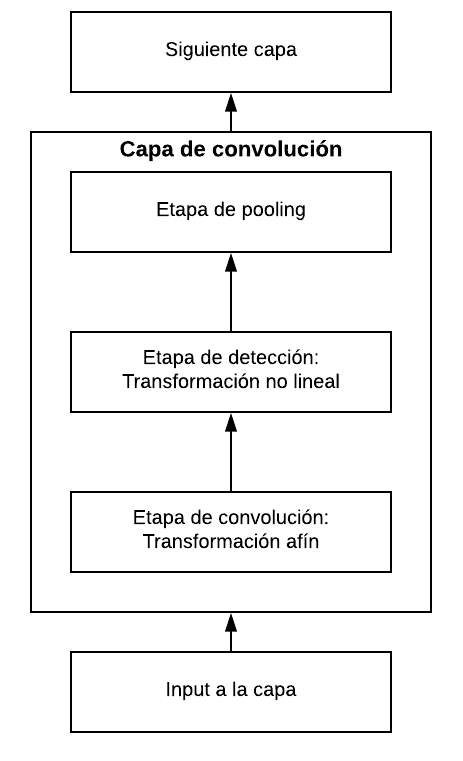
\includegraphics[scale=.8]{img/CNN.png}
\end{figure}

\textbf{Max pooling} retorna el valor m\'aximo de un output en una vecindad rectangular. Las operaciones de pooling permiten que la red sea invariante a peque{\~{n}}as transformaciones en el input. Pooling tambi\'en es escencial para procesar inputs de tama{\~{n}}o variable (por ejemplo im\'agenes de distinto tama{\~{n}}o).

Otras diferencias con respecto a la operaci\'on de convoluci\'on en el contexto de redes neuronales son, por ejemplo, el aplicar m\'ultiples convoluciones en paralelo, esto permite extraer distintos tipos de atributos en vez de 1 solo. Por otro lado, el \textbf{stride} hace referencia a cada cu\'antos pixeles se quieren convolucionar en cada direcci\'on en el output. En la figura se muestra el ejemplo de una convoluci\'on con stride. Esta operaci\'on permite reducir nuevamente el costo computacional. Esto tambi\'en implica que el output disminuye su tama{\~{n}}o en cada capa. El uso de \textit{padding} puede revertir esto. \textbf{Padding} se refiere a agrandar el input con ceros para hacerlo m\'as amplio. Una convoluci\'on en la que no se usa \textbf{zero-padding} se conoce como \textbf{valid}. Una convoluci\'on que mantiene el tama{\~{n}}o desde el input al output se conoce como \textbf{same} (ver figura). En la pr\'actica, las capas de una red convolucional usan operaciones entre una convoluci\'on valid y same.

\begin{figure}[H]
\captionsetup{font=small,labelfont=small}
\caption{Convoluci\'on con un stride igual a 2}
\centering
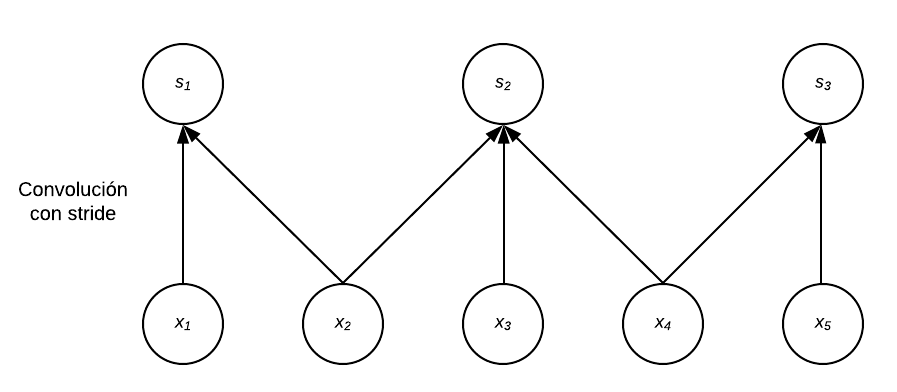
\includegraphics[scale=.8]{img/stride.png}
\end{figure}

\begin{figure}[H]
\captionsetup{font=small,labelfont=small}
\caption{Efecto de no usar zero-padding en una red convolucional (Arriba) y efecto de usar zero padding en una red convolucional (Abajo) en cuanto al tama{\~{n}}o de la red}
\centering
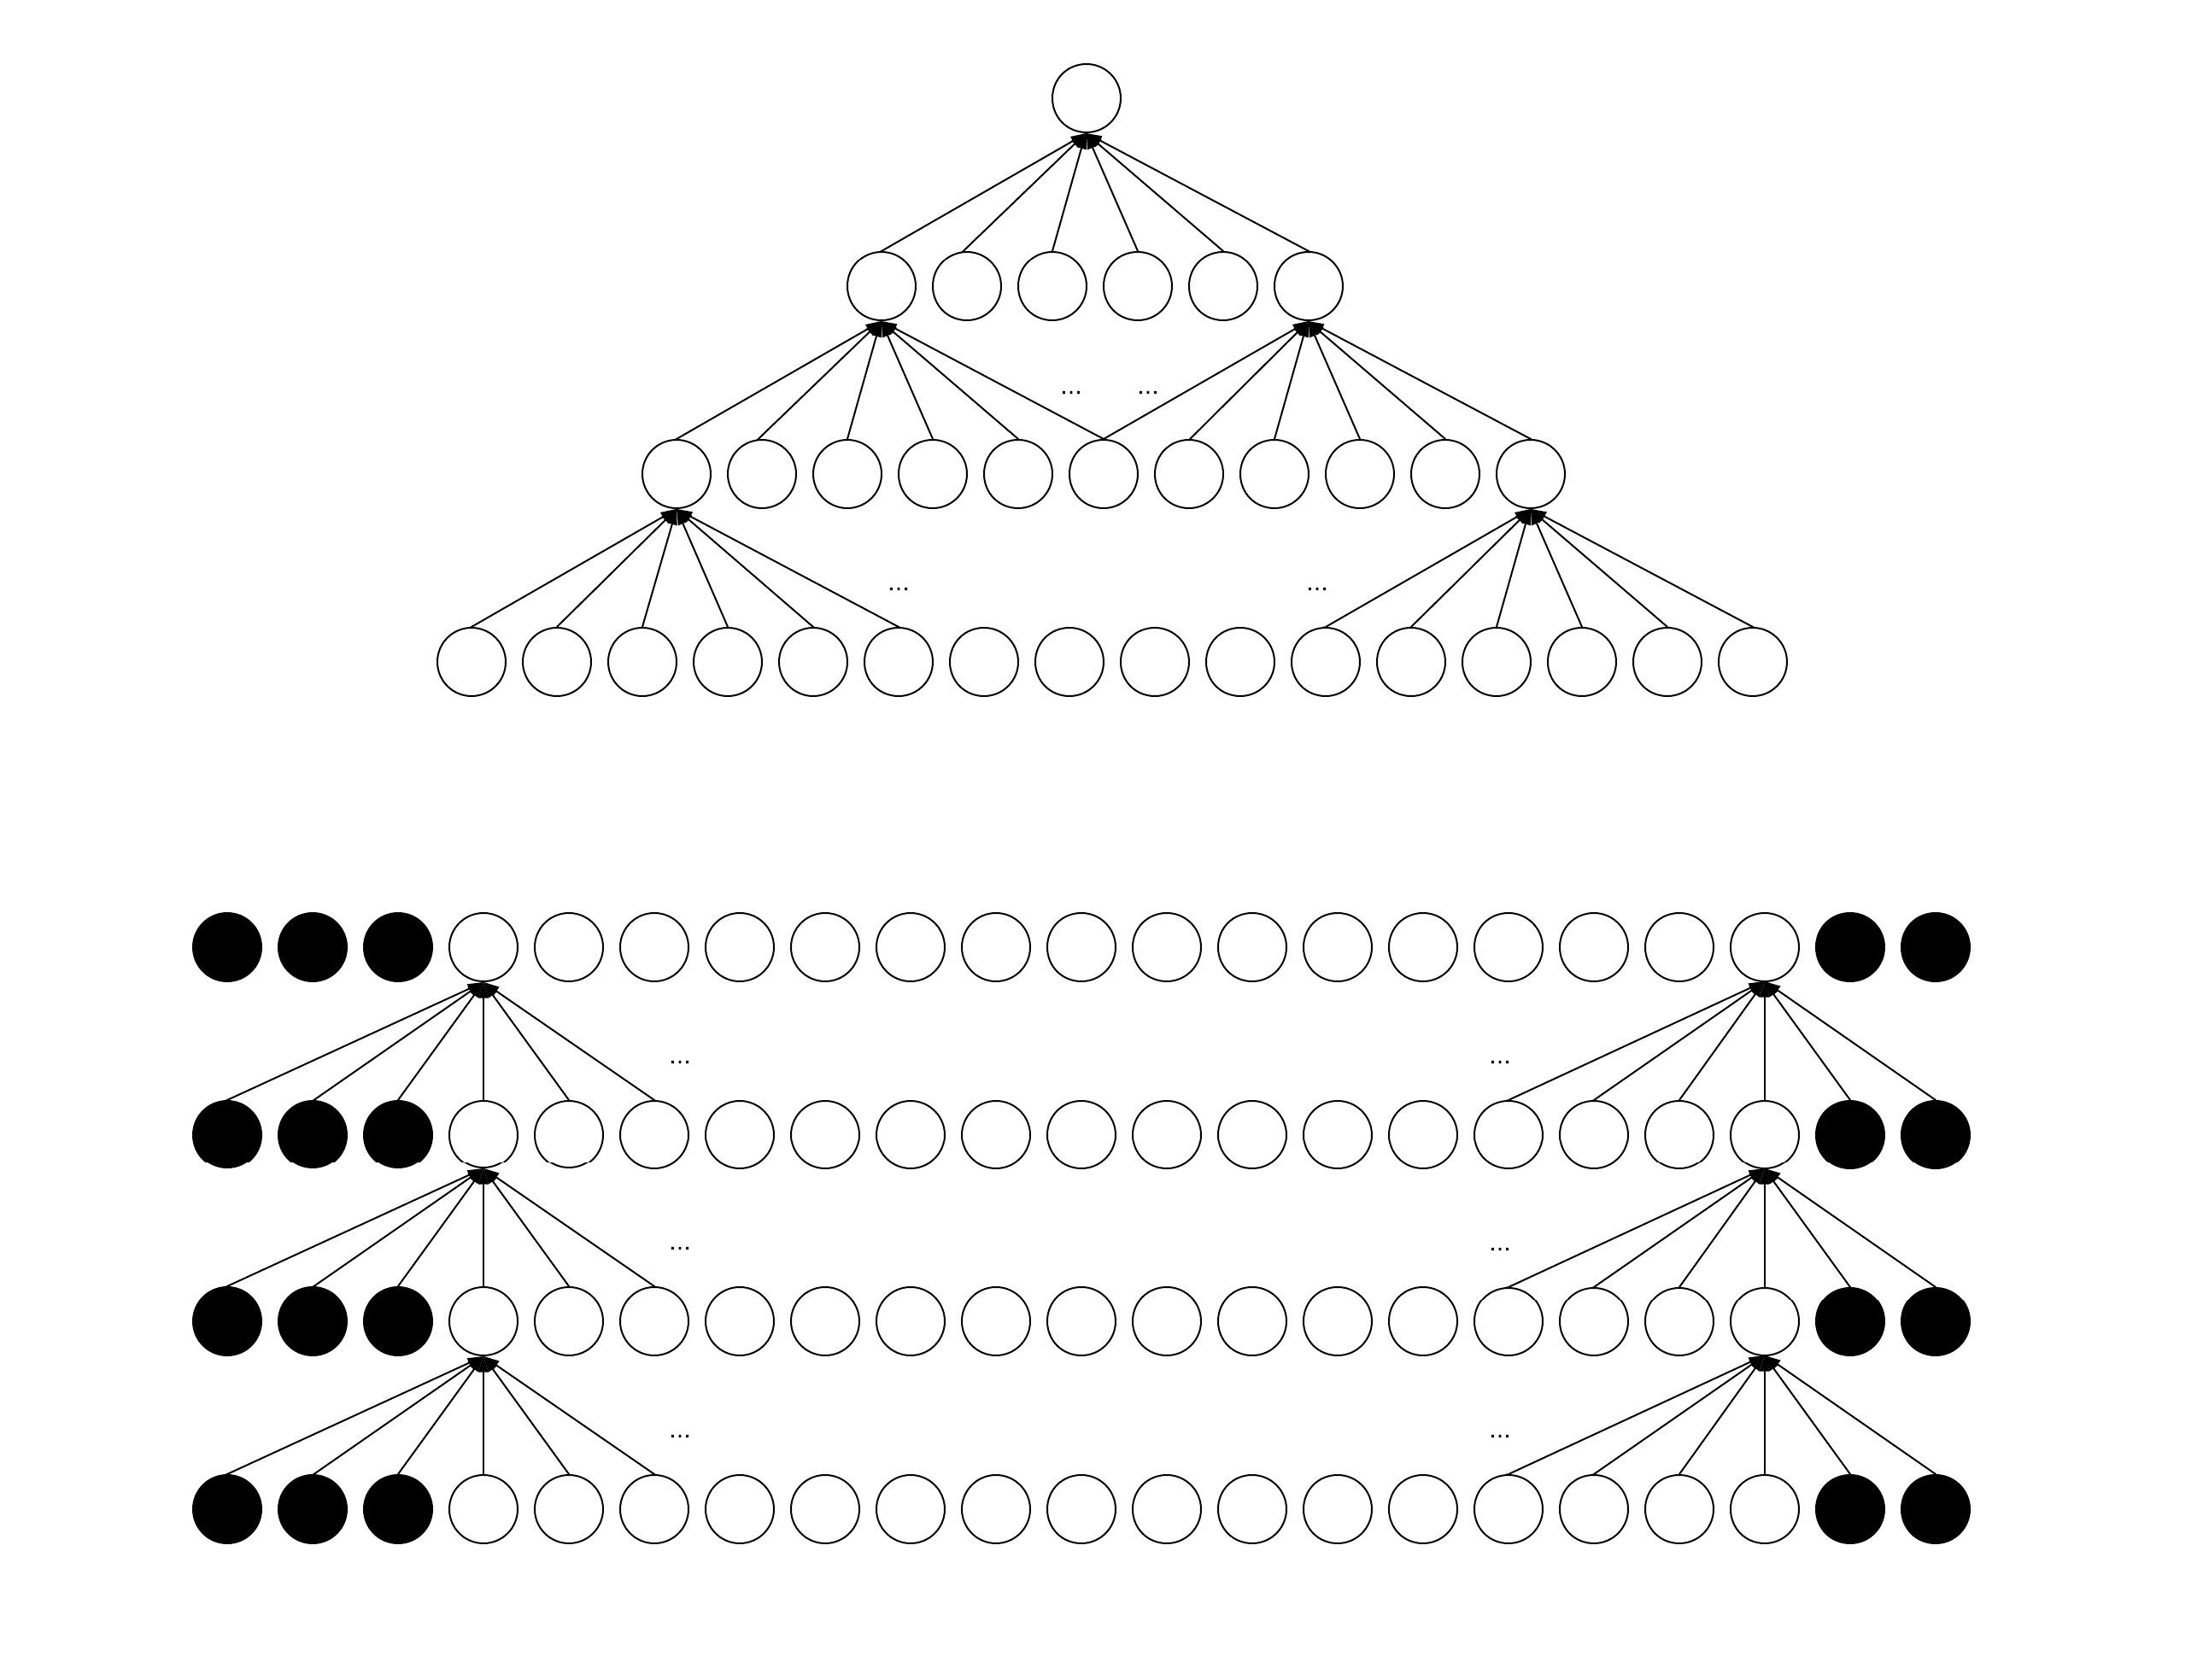
\includegraphics[scale=.15]{img/padding.png}
\end{figure}

\subsubsection{Redes Neuronales Recurrentes}

Las \textbf{redes neuronales recurrentes} o \textbf{RNNs} son una familia modelos de redes neuronales especializados para procesar datos secuenciales, $\bm{x}^{(1)},...,\bm{x}^{(\tau)}$. Las RNNs tambi\'en comparten par\'ametros, pero en una forma muy distinta que las CNNs. En una RNN, cada miembro del output en una etapa es una funci\'on de cada miembro del output de la etapa anterior.

Se denota por $\bm{h}^{(t)}$ al estado de un sistema din\'amico que involucra una recurrencia conducido por un input externo $\bm{x}^{(t)}$:

\begin{equation}
\bm{h}^{(t)} = f(\bm{h}^{(t-1)}; \bm{x}^{(t)}, \bm{\theta})
\end{equation}

La figura siguiente muestra una red recurrente que procesa un input $\bm{x}$ incorpor\'andolo al estado $\bm{h}$ que es traspasado a trav\'es del tiempo.

\begin{figure}[H]
\captionsetup{font=small,labelfont=small}
\caption{Ejemplo de una red recurrente sin output}
\centering
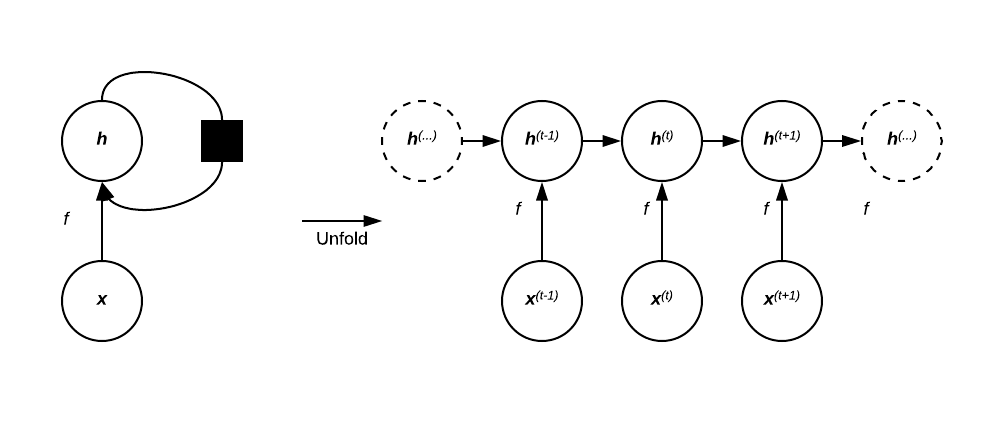
\includegraphics[scale=.5]{img/RNN1.png}
\end{figure}

Las redes recurrentes se pueden construir de muchas formas distintas. Al igual que una red neuronal puede representar casi cualquier funci\'on, una red recurrente modela cualquier funci\'on que involucre una recurrencia. Se puede representar el estado de una red recurrente luego de $t$ pasos mediante una funci\'on $g^{(t)}$:

\begin{equation}
\bm{h}^{(t)} = g^{(t)}(\bm{x}^{(t)},\bm{x}^{(t-1)},...,\bm{x}^{(1)}) =  f(\bm{h}^{(t-1)}; \bm{x}^{(t)}, \bm{\theta})
\end{equation}

Existen varios tipos de RNNs que se han dise{\~{n}}ado para distintos fines. Algunos ejemplos de estas son:

\begin{itemize}
  \item Redes recurrentes que producen un output en cada instante de tiempo y tienen conexiones entre todas las unidades escondidas
  \item Redes recurrentes que producen un output en cada instante de tiempo y tienen conexiones entre el output a la unidad escondida del siguiente instante
  \item Redes recurrentes con conexiones entre las unidad escondidas, que procesan una secuencia entera antes de producir el output
\end{itemize}

La figura muestra un ejemplo de la arquitectura para el primer caso.

\begin{figure}[H]
\captionsetup{font=small,labelfont=small}
\caption{Ejemplo de una red recurrente que produce un output en cada instante de tiempo, y que comparte el estado a trav\'es del tiempo}
\centering
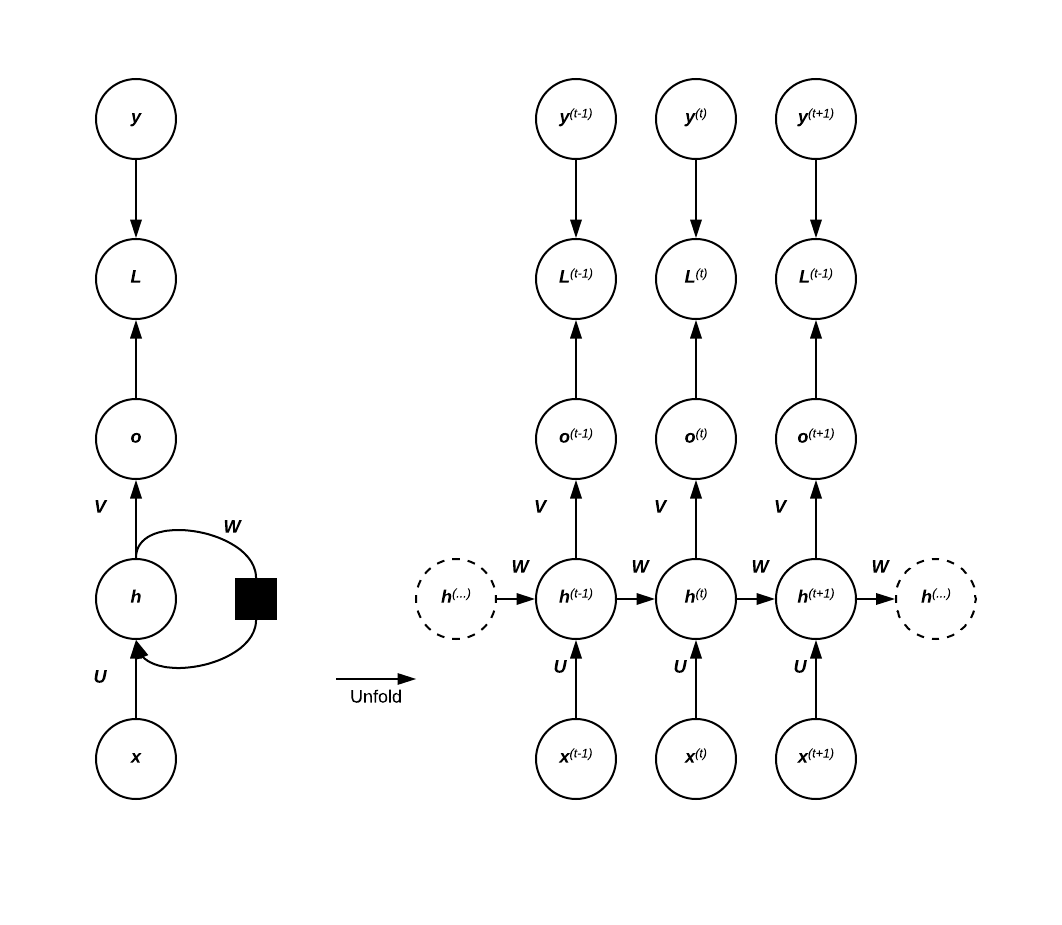
\includegraphics[scale=.5]{img/RNN2.png}
\end{figure}

Esta red presentada puede ser usada para producir palabras en cada instante, y as\'i producir oraciones que hagan sentido en una conversaci\'on. Como ejemplo de entrenamiento de una red con esta arquitectura, en donde en la \'ultima capa se decide mediante una funci\'on softmax la palabra m\'as probable que deba seguir a la palabra anterior, se tienen las ecuaciones de \textit{forward propagation} para cada instante de tiempo:

\begin{equation}
\begin{array}{l}
\bm{a}^{(t)} = \bm{b} + \bm{W}\bm{h}^{(t-1)}+\bm{U}\bm{x}^{(t-1)} \\
\bm{h}^{(t)} = \textrm{tanh}(\bm{a}^{(t)}) \\
\bm{o}^{(t)} = \bm{c} + \bm{V}\bm{h}^{(t)} \\
\hat{\bm{y}}^{(t)} = \textrm{softmax}(\bm{o}^{(t)})
\end{array}
\end{equation}

El algoritmo aplicado para obtener el gradiente en este tipo de arquitectura se conoce como \textbf{back-propagation through time}, y consiste en aplicar el algoritmo de \textit{back-propagation} generalizado para el grafo computacional \textit{unfolded} de la red, como los mostrados en las figuras de redes recurrentes.

Las redes recurrentes sufren de no poder recordar largas dependencias a trav\'es del tiempo, debido a que las recurrencias implican multiplicar una matriz de pesos m\'ultiples veces a trav\'es de la red, provocando superficies planas o muy empinadas que resultan en que los algoritmos de aprendizaje por gradiente tengan problemas de \textbf{vanishing gradients} o \textbf{exploding gradients}, respectivamente. Arquitecturas que han logrado superar esto son las que incluyen compuertas (funciones sigmoidales) que deciden autom\'aticamente qu\'e olvidar y qu\'e seguir propagando a trav\'es de la red. Estos son los modelos de \textbf{gated recurrent units} (\textbf{GRUs}) y \textbf{long-short term memory network} (\textbf{LSTM}).

\subsubsection{Autoencoders}

Un \textbf{autoencoder} es una red neuronal que busca replicar el input hacia el output, osea, se busca que la información que entra a la red sea lo más parecida posible a la de salida, para lo cual cuenta con una capa interna $\bm{h} = f(\bm{x})$ que codifica el input (genera una representaci\'on de este) llamada \textbf{encoder} y una funci\'on que produce la reconstrucci\'on $\bm{r} = g(\bm{h})$, el \textbf{decoder}. Un \textit{autoencoder} buscar\'a aprender los \textit{encoder} y \textit{decoder} tales que $g(f(\bm{x})) = \bm{x}$ para todo $\bm{x}$. Como el modelo est\'a forzado a aprender los atributos m\'as importantes para que pueda efectivamente reproducir el input en su output, este aprender\'a en general propiedades \'utiles de los datos de entrenamiento. Los \textit{autoencoders} modernos modelan mappings estoc\'asticos $p_{\textrm{encoder}}(\bm{h}|\bm{x})$ y $p_{\textrm{decoder}}(\bm{x}|\bm{h})$, en vez de funciones determin\'isticas. En la figura se muestra la arquitectura de un \textit{autoencoder}.

\begin{figure}[H]
\captionsetup{font=small,labelfont=small}
\caption{Estructura de un \textit{autoencoder} t\'ipico}
\centering
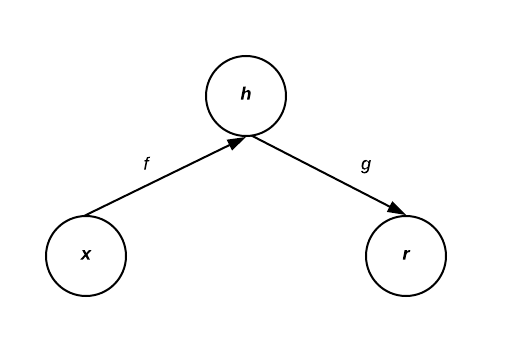
\includegraphics[scale=.8]{img/autoencoder.png}
\end{figure}

Una manera de obtener atributos \'utiles de $\bm{x}$ es forzando a que el \textit{encoder} tenga una dimensionalidad menor que el input. Este tipo de \textit{autoencoders} se denominan \textbf{undercomplete}. El aprendizaje se describe mediante la optimizaci\'on de la funci\'on de p\'erdida, $L(\bm{x}, g(f(\bm{x})))$. Cuando el \textit{decoder} es lineal y la funci\'on de p\'erdida es el error cuadr\'atico medio, un \textit{undercomplete autoencoder} aprende a generar el mismo subespacio que el algoritmo \textbf{principal component analysis} (\textbf{PCA}), es decir, el \textit{autoencoder} que fue entrenado para reproducir los datos de entrenamiento mediante una reducci\'on de dimensionalidad y una reconstrucci\'on aprendi\'o como efecto colateral el subespacio principal. Es as\'i como entonces, \textit{autoencoders} con \textit{encoders} y \textit{decoders} no lineales pueden aprender representaciones no lineales m\'as poderosas que PCA.

Un \textit{autoencoder} con dimensi\'on de su \textit{encoder} igual a la del input se conoce como \textbf{overcomplete}. Estos \textit{autoencoders}, al igual que los \textit{undercomplete}, pueden fallar en aprender una representaci\'on \'util del input si tienen mucha capacidad, por lo que ser\'a importante tambi\'en regularizar estas redes neuronales.

Otras aplicaciones de los autoencoders, aparte de aprender una reducci\'on de dimensionalidad, es aprender representaciones \'utiles que sirvan para un posterior modelo de redes neuronales (o, m\'as general, de aprendizaje de m\'aquinas). Por ejemplo, en vez de usar \textbf{one-hot-vectors} para representar palabras (en donde se tiene un vector del largo de cierto vocabulario compuesto por ceros excepto para la palabra que se quiere representar, indicando un valor de 1 en esa posici\'on), se pueden usar \textbf{embeddings}, que son representaciones del input a un espacio de valores reales. A diferencia de los \textit{one-hot-vectors}, en un \textit{embedding} la distancia entre las representaciones del texto s\'i tiene un significado, y este tipo de representaciones podr\'ia entregar mejores resultados en la tarea en que se est\'e usando.

\subsubsection{Redes Generativas Adversariales}

Una \textbf{red generativa adversarial} (o \textbf{GAN}) se basa en un escenario de teor\'ia de juegos, en donde una \textbf{red generadora} debe competir con un adversario. La red generadora produce muestras $\bm{x} = g(\bm{z};\bm{\theta}^{(g)})$, mientras que una \textbf{red discriminadora} trata de distinguir entre muestras obtenidas de los datos de entrenamiento y muestras generadas por la red generadora. El discriminador retorna una probabilidad, $d(\bm{x};\bm{\theta}^{(d)})$, indicando la probabilidad de que $\bm{x}$ sea un dato real y no uno simulado.

Para formuuar el aprendizaje, se describe un juego de suma cero en donde una funci\'on $v(\bm{\theta}^{(g)},\bm{\theta}^{(d)})$ determina el pago del discriminador, y el generador recibe $-v(\bm{\theta}^{(g)},\bm{\theta}^{(d)})$ como pago. As\'i, durante el entrenamiento cada jugador intenta maximizar su propio pago, para que en convergencia se tenga

\begin{equation}
g^{*} = \textrm{arg} \textrm{min}_{g} \textrm{max}_{d} v(g,d)
\end{equation}

Esto motiva a que el discriminador aprenda a clasificar correctamente entre muestras reales y falsas y, simulat\'aneamente, el generador intenta enga{\~{n}}ar al clasificador para que crea que las muestras generadas son reales. En convergencia, las muestras del generador son indistinguibles de los datos reales. Una motivaci\'on del uso de GANs es que cuando $\textrm{max}_{d} v(g,d)$ es convexa en $\bm{\theta}^{(g)}$, el procedimiento asegura la convergencia.

\begin{figure}[H]
\captionsetup{font=small,labelfont=small}
\caption{Im\'agenes generadas por una GAN entrenada con el set de datos LSUN. (Izquierda) Im\'agenes de dormitorios generadas por el modelo DCGAN (imagen de Radford et al., 2015). (Derecha) Im\'agenes de iglesias generadas por el modelo LAPGAN (imagen de Denton et al., 2015)}
\centering
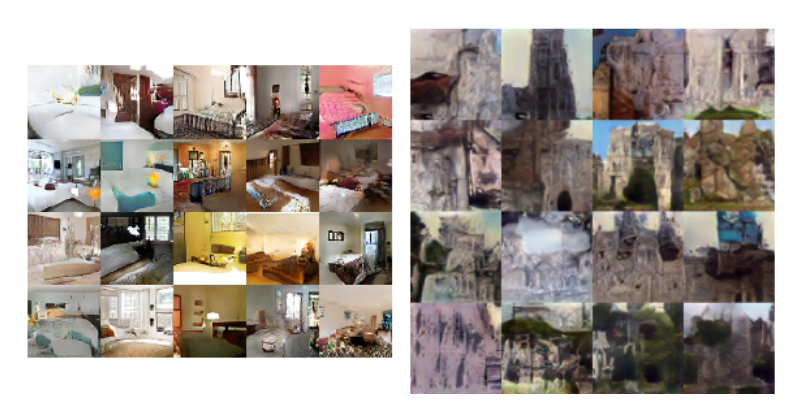
\includegraphics[scale=.75]{img/gans.PNG}
\end{figure}\newpage
%!TEX root = notas_de_clase.tex


\section{Support Vector Machines}

\subsection{Introducción}
\label{sub:svm_intro}

En este capítulo del apunte, discutiremos las llamadas \textbf{máquinas de soporte vectorial} (SVM) que constituyen un set de herramientas para resolver el problema de clasificación de datos. Fue desarrollada en los 90 dentro de la comunidad de computer science y ha crecido enormemente desde entonces. Esta técnica ha demostrado ser útil en diversos escenarios, y es considerado uno de los mejores clasificadores para ``llegar y usar''. 

\subsection{Idea general}


Los SVM son una generalización de un clasificador más simple e intuitivo llamado el clasificador de márgen máximo (\textit{maximum margin classifier})

Para estudiar dicho clasficador, comenzaremos estudiando el caso en que tenemos que clasificar los datos en dos grupos, y además supondremos que los datos son linealmente separables (es decir, existe un hiperplano que los separa, ver fig.~\ref{fig:maxim_marg}). Esto último es claramente un supuesto muy fuerte, pero lo generalizaremos mas adelante. 


\begin{figure}[ht]
    \centering
    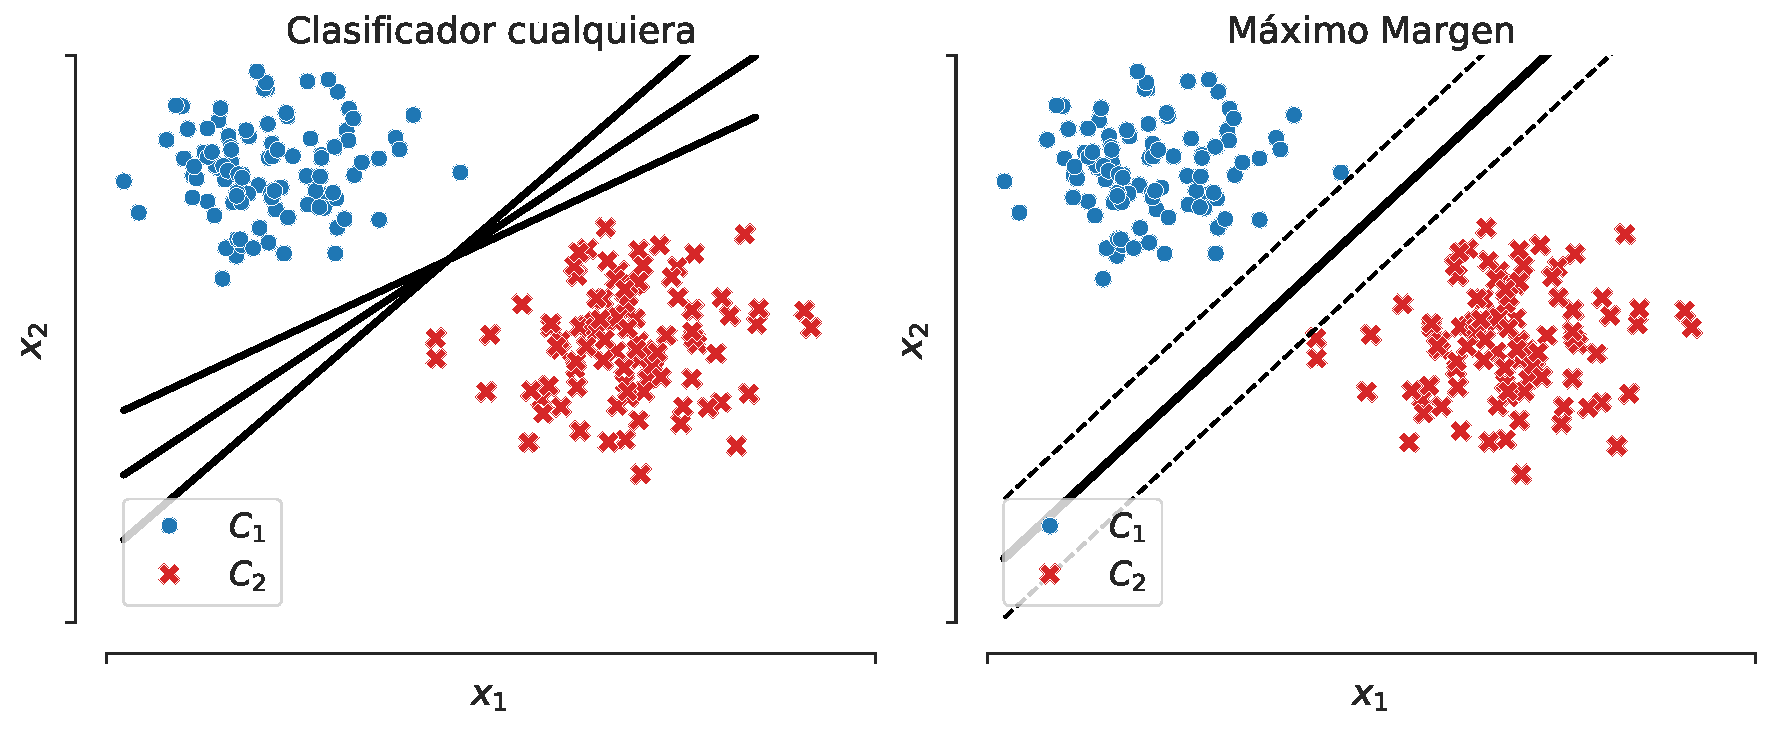
\includegraphics[width=0.9\textwidth]{img/cap5_max_margen.pdf}
    \caption{Modelo de máximo margen entre los datos}
    \label{fig:maxim_marg} 
\end{figure}


Como se puede apreciar en la fig.~\ref{fig:maxim_marg} (centro), dados puntos linealmente separables, existen diferentes hiperplanos que separan los datos. Cada una de estas líneas define un modelo, ya que dado un nuevo dato $x^*$, si este está por encima de la línea, entonces es un dato verde, en cambio si esta por debajo, entonces es un dato rojo. 
\\

¿Cuál elegir?
\\

Estudiaremos una respuesta natural al problema: ¿cómo elegir el hiperplano que nos entregue el \textbf{mayor margen} posible entre ambos grupos? Esto se traduce en reemplazar el problema de separar mediante una línea, en separar mediante una \emph{cinta} de ancho máximo. A este modelo se le llama el separador de máximo margen que mencionamos antes. 
\\

El argumento de ocupar dicho modelo es que uno esperaría que si un modelo tiene un buen margen en los datos de entrenamiento, entonces el \textbf{error de generalización} (Cuanto se equivoca el modelo con datos nuevos) debiese ser bajo. Existe un argumento matemático, y a grandes rasgos es que a mayor margen y a medida aumentan los datos,  podemos acotar la probabilidad de error (Al estilo desigualdad de Markov) sin embargo los detalles se escapan de los contenidos del curso.  
\\

Continuando, en la fig.~\ref{fig:maxim_marg} (derecha) podemos visualizar el modelo. Notar que el  margen esta definido solamente por algunos puntos. En la figura son dos, podrían ser más, pero nunca menos por la naturaleza `` simétrica '' del modelo.
\\

Dichos puntos que definen el márgen son llamados los vectores de soporte (support vectors) que le entregan el nombre al método. 
\\

Un ejemplo sencillo para recordar que es lo que hace SVM es imaginar que el ejemplo de los gráficos trata sobre clasificar manzanas y naranjas: 


A diferencia de otros métodos que aprenden analizando todos los datos y llegando a una respuesta (Cómo Naive Bayes, Regresión Lineal, etc...) de lo que en promedio podría ser una manzana, SVM mira la manzana mas naranjezca y la naranja mas manzanezca y con esos datos define un hiperplano separador. 



\begin{figure}[ht]
    \centering
    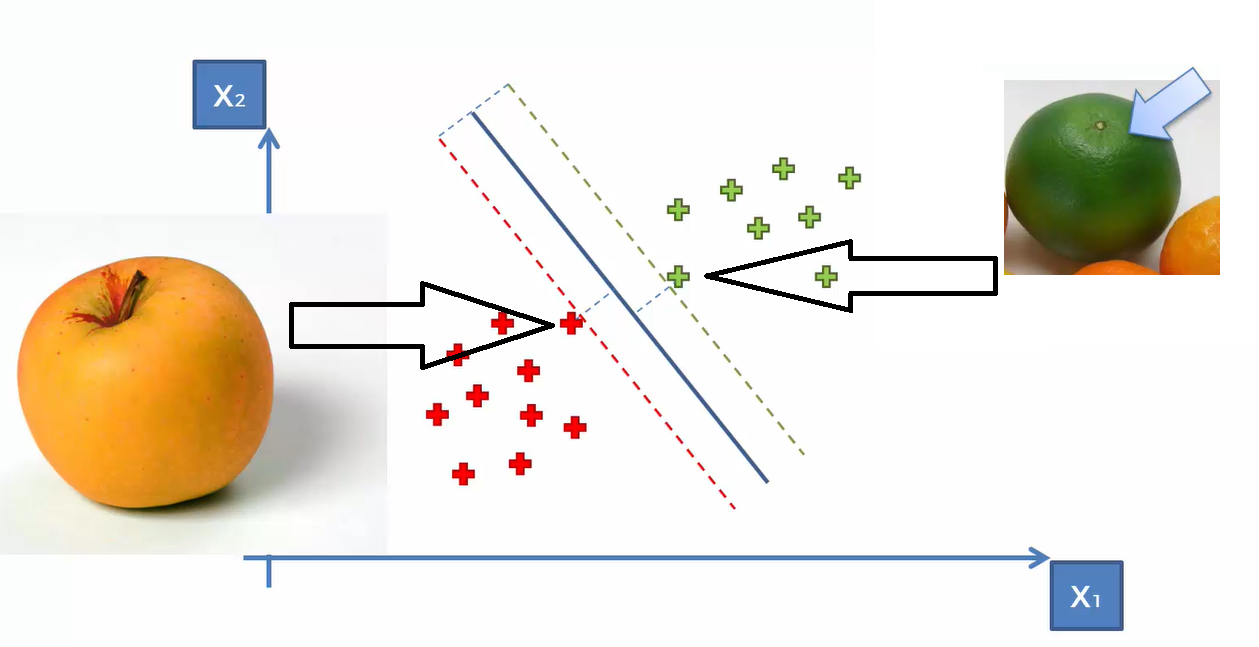
\includegraphics[scale=0.3]{img/img5.png}
    \caption{Los vectores de soporte son la manzana más naranjezca y la naranja más manzanezca}
    \label{fig:my_label1}
\end{figure}

\subsection{Problema}



Como ya mencionamos tenemos datos de entrenamiento $\{x_i\}_{1,...,N}$ que suponemos linealmente separables y deseamos encontrar un hiperplano de máximo margen que los separe. 

Un hiperplano en general son los $x\in \R^n$ que cumplan al ecuación

\begin{equation}
    w\cdot x + b = 0 
\end{equation}

Donde $w\in \R^n$ es el vector perpendicular al hiperplano y $b\in \R$ es un parámetro. La idea es encontrar $w$ y $b$ tales que entreguen el hiperplano separador de mayor margen. Este problema no tiene solución única (Pues si $w$ es solución entonces $\lambda w$ también). Para evitar ese problema, escalamos el plano de manera que los vectores de soporte ($x_{+}$ y $x_{-}$) sean tales que $w\cdot x_{+} + b = 1$ y $w\cdot x_{-} + b =  -1$ (Pueden haber mas vectores de soporte, pero para efectos del cálculo usaremos dos). Si bien aún no tenemos los vectores de soporte para hacer el escalamiento, este será parte de las restricciones del problema de optimización que resolveremos. 

El márgen del hiperplano es la mitad de la diferencia entre ambos vectores de soporte, proyectada en la dirección $\frac{w}{||w||}$ (Ver figura 5). 

\begin{figure}[ht]
    \centering
    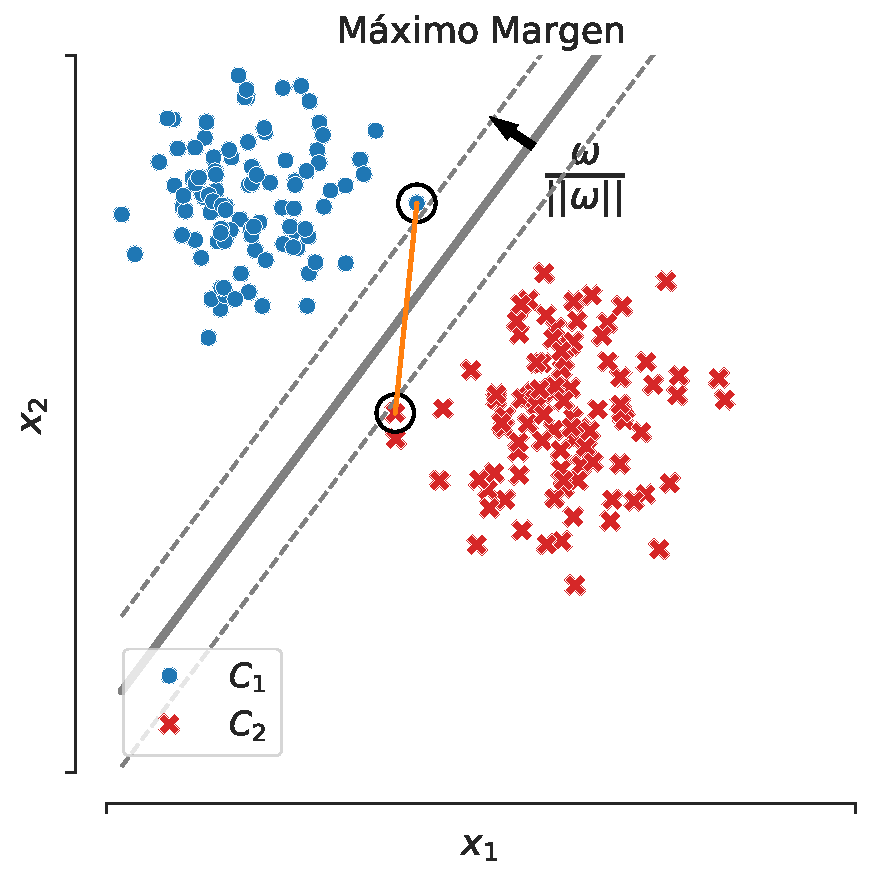
\includegraphics[width=0.4\textwidth]{img/cap5_max_margen2.pdf}
    \caption{En azul los vectores $x_+$ y $x_{-}$. En rojo el vector $(x_+ - x_{-})$. En naranjo la componente del vector rojo, proyectada en la dirección definda por $\frac{w}{||w||}$. Notar que corresponde justamente al doble del margen}
    \label{fig:my_label2}
\end{figure}

Calculamos:

\begin{align*}
    \frac{1}{2||w||}[ w \cdot (x_{+} - x_{-})] &= \frac{1}{2||w||} [ (w\cdot x_{+}) - (w\cdot x_{-})]\\
    &= \frac{1}{2||w||} [1 - (-1)]\\
    &= \frac{1}{||w||}
\end{align*}

Definiendo a $y_i$ como $1$ si $w\cdot x_i + b \geq1$ y $y_i =-1$ cuando  $w\cdot x_i + b \leq -1$, podemos formular el problema del hiperplano de margén máximo como

\begin{equation*}
\begin{aligned}
& \underset{w,b}{\text{max}}
& & \frac{1}{||w||}\\
& \text{s.a}
& & y_i (w\cdot x_i +b) \geq 1, \; i = 1, \ldots, N.
\end{aligned}
\end{equation*}

Para evitar problemas de diferenciablidad, en realidad se ocupa la siguiente formulazión equivalente

\begin{equation*}
\begin{aligned}
& \underset{w,b}{\text{min}}
& & \frac{1}{2}||w||^2\\
& \text{s.a}
& & y_i (w\cdot x_i +b) \geq 1, \; i = 1, \ldots, N.
\end{aligned}
\end{equation*}

Ahora estudiaremos el lagrangiano del problema (Y en consecuencia su dual). Este problema tiene una mejor estructura para optimizar, además que nos servirá para generalizar al caso no lineal. 

El lagrangiano es

\begin{equation*}
    L(w,b,\alpha) = \frac{1}{2}||w||^2 - \sum\limits_{i=1}^{N} \alpha_i (y_i (w\cdot x_i +b) -1)
\end{equation*}

Las condiciones de primer orden nos dicen que

\begin{equation}
    \dfrac{\partial L}{\partial w} = 0 \Rightarrow w = \sum\limits_{i=1}^{N} \alpha_i y_i x_i
\end{equation}

\begin{equation}
    \dfrac{\partial L}{\partial b} = 0 \Rightarrow \sum\limits_{i=1}^{N} \alpha_i y_i = 0 
\end{equation}


Reemplazando $(2)$ y $(3)$ en $L(w,b, \alpha)$, maximizando (por ser dual) e imponiendo holgura complementaria, el problema queda

\begin{equation*}
\begin{aligned}
& \underset{\alpha}{\text{max}}
& & \sum\limits_{i=1}^{N}\alpha_i - \frac{1}{2} \sum\limits_{i,j=1}^{N} \alpha_i \alpha_j y_i y_j \langle x_i, x_j\rangle\\
& \text{s.a}
& & \sum\limits_{i=1}^{N} \alpha_i y_i= 0 \\
& &  &\alpha_i \geq 0
\end{aligned}
\end{equation*}

Este problema es de la forma QP (Quadratic Programming) y existen diferentes métodos para resolverlo de manera óptima. 
Notar la participación del producto punto $\langle\cdot, \cdot\rangle$ en este problema, pues este será el punto de partida del SVM no lineal. 

Una vez resuelto el dual, la predicción de un nuevo punto $x^*$ es de la forma $$\hat{y}(x^*)= \text{sgn}\left(\left[\sum\limits_{i=1}^{N} \alpha_i y_i \langle x_i, x^*\rangle\right] - b\right)$$

Por holgura complementaria tenemos que si $x_i$ no está en el márgen, entonces $\alpha_i = 0$ de modo que $x_i$ no aporta en la predicción $\hat{y}$. Esta propiedad es la que mencionabamos al principio: La predicción solo depende de los vectores de soporte. 

Esta propiedad ayuda a resolver el problema de optimización de manera más rápida, ya que en realidad solo algunas variables duales $\alpha_i$ serán no nulas. Normalmente se ocupan heurísticas para encontrar rápidamente que vectores no son de soporte y así resolver un problema mas pequeño (Buscar, por ejemplo, el método de Sequential Minimal Optimization) 



\subsection{Soft Margin}


El planteamiento anterior tiene dos debilidades. Una, la más obvia, es que no siempre podemos tener datos separables y la segunda es que, incluso si los datos son linealmente separables, nuestro clasificador puede ser muy sensible a nuevos datos. Ver por ejemplo la Fig.\ref{fig:my_label3}.

\begin{figure}[ht]
    \centering
    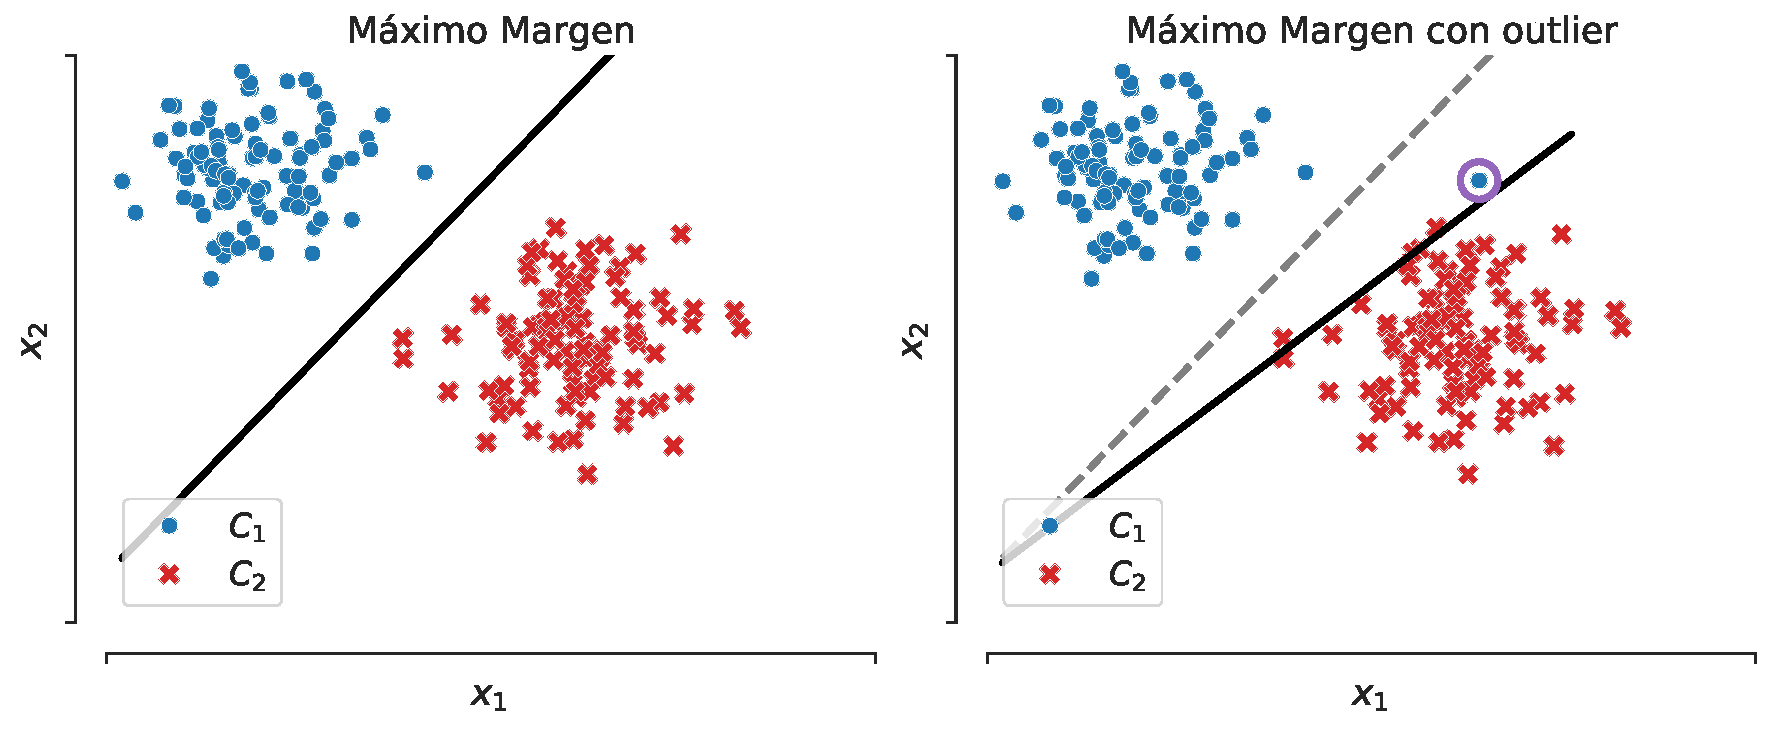
\includegraphics[width=0.9\textwidth]{img/cap5_margen_suave}
    \caption{Sensibilidad del máximo margen al agregar un nuevo dato.}
    \label{fig:my_label3}
\end{figure}


Como se ve en la imagen, la llegada del nuevo dato (encerrado en rojo) cambia drásticamente nuestro modelo. 

Para solucionar estos problemas (parcialmente) agregamos variables de holgura, que nos permitirán clasificar mal algunos datos. La idea es que, sacrificando algunos datos (muy probablemente outliers), podamos clasificar mejor la \textit{mayoría} de los datos (Clasificarlos todos era claramente muy ambicioso) y así tener un modelo mas robusto.  


Dicha formulazión del problema es la siguiente:

\begin{equation*}
\begin{aligned}
& \underset{w,b, \xi}{\text{min}}
& & \frac{1}{2}||w||^2 + c\sum\limits_{i=1}^{N} \xi_i \\
& \text{s.a}
& & y_i (w\cdot x_i +b) \geq 1 - \xi_i, \; i = 1, \ldots, N.
\end{aligned}
\end{equation*}

donde $c$ es un parámetro (Ya hablaremos de él).

Los $\xi$ indican que tan mal clasificado está un punto. Si $\xi_i = 0$, entonces el dato $x_i$ está al lado correcto del plano. Si $0<\xi_i <1$, entonces $x_i$ está al lado correcto del plano, pero viola la restricción del margen. Finalmente si $\xi_i>1$, entonces el punto esta al lado incorrecto del plano (Ver la siguiente figura)

\begin{figure}[ht]
    \centering
    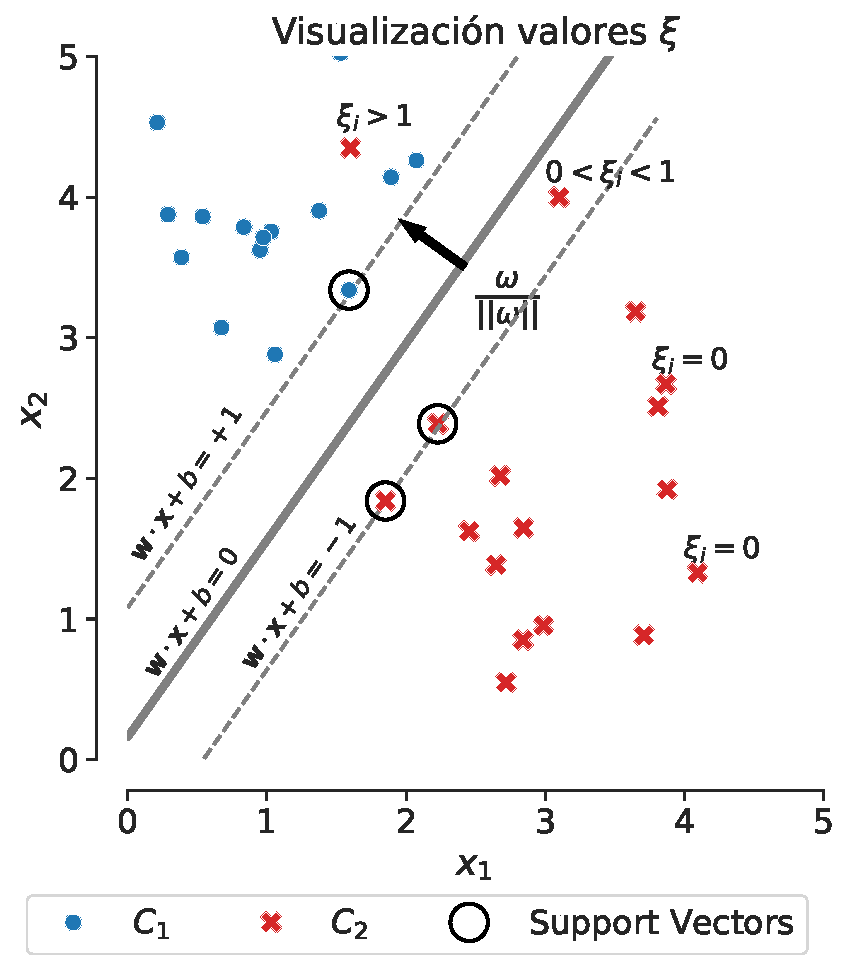
\includegraphics[width=0.45\textwidth]{img/cap5_max_margen3}
    \caption{Visualización de los valores de $\xi$}
    \label{fig:my_label4}
\end{figure}

El dual de este problema es (Usando Lagrangiano etc.)

\begin{equation*}
\begin{aligned}
& \underset{\alpha}{\text{max}}
& & \sum\limits_{i=1}^{N}\alpha_i - \frac{1}{2} \sum\limits_{i,j=1}^{N} \alpha_i \alpha_j y_i y_j \langle x_i, x_j\rangle\\
& \text{s.a}
& & \sum\limits_{i=1}^{N} \alpha_i y_i= 0 \\
& &  &0 \leq \alpha_i \leq c
\end{aligned}
\end{equation*}

Volveremos a este dual cuando veamos métodos no lineales. 
\\

Por último, ¿Qué hacer con el parámetro $c$? Guarda relación con el \textit{bias-variance tradeoff}. La variable $c$ es un parámetro de tolerancia. A mayor $c$, encontraremos un mayor márgen, lo que significa que nuestro modelo no estará sumamente ajustado a los datos (Lo que lo vuelve mas insesgado), pero probablemente se equivoque más (Tenga mayor varianza). Al revés, un $c$ muy pequeño nos llevará más cerca del caso inicial, donde nuestro margen será más pequeño, y por ende, raramente violado (Poca varianza), pero nuestro modelo podría quedar sobreajustado a nuestros datos, logrando un mayor sesgo.En la práctica se usa \textit{cross-validation} para encontrar un buen parámetro $c$.  


\subsection{Kernel Methods}

Los métodos anteriores se ven interesantes, pero podría desmotivar el hecho que sólo funciona para datos linealmente separables (Con un poco de holgura en el caso de soft margin). 

Un caso particular es el problema de clasificación XOR que se muestra en la siguiente figura

\begin{figure}[ht]
    \centering
    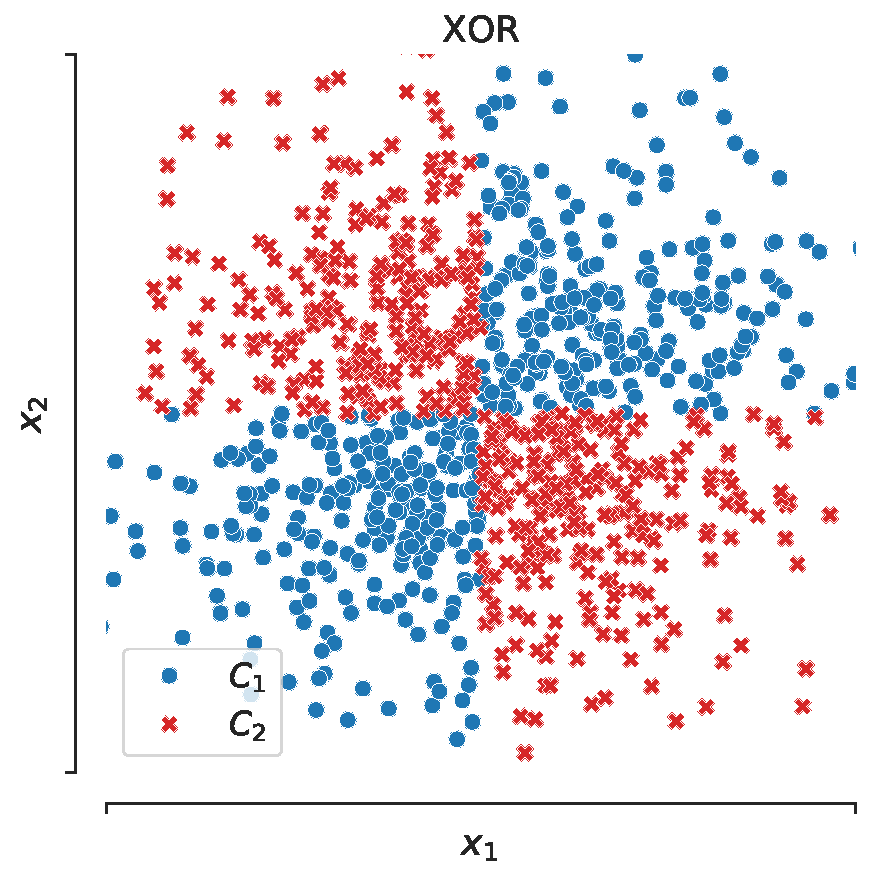
\includegraphics[width=0.45\textwidth]{img/cap5_xor}
    \caption{Datos XOR no son linealmente separables}
    \label{fig:my_label5}
\end{figure}

Dichos datos no son linealmente separables en $\R^2$, pero si consideramos el siguiente mapeo a $\R^3$

\begin{equation}
    \phi(x_1, x_2) = (x_1, x_2, x_1 x_2)
\end{equation}

Entonces es claro que el plano $z=0$ en $\R^3$ será capaz de separar dichos puntos (Pues si $x_1 x_2 > 0$ entonces dicho punto será rojo y estará por sobre el plano $z=0$, y análogamente sucede algo similar con los puntos azules). 

\begin{figure}[ht]
    \centering
    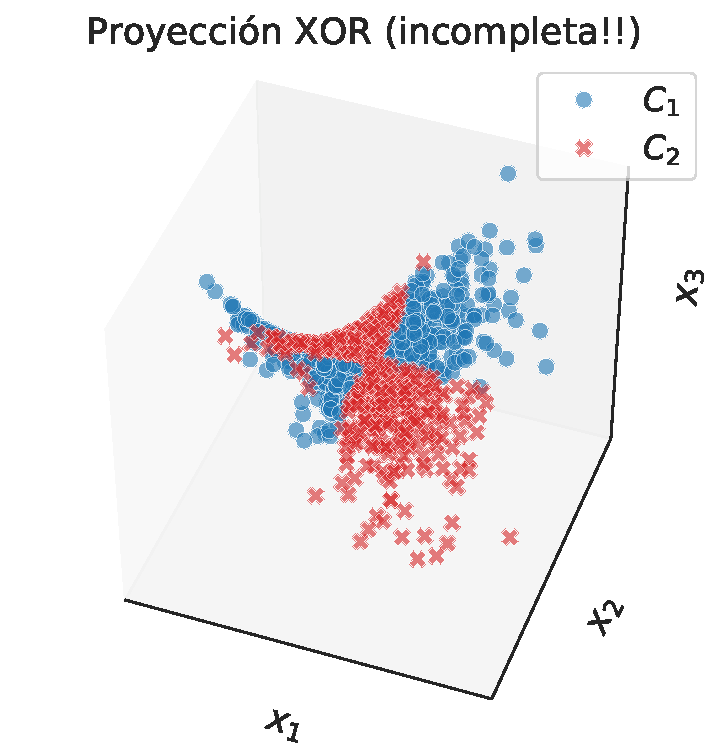
\includegraphics[width=0.45\textwidth]{img/cap5_xor_3d_proyeccion}
    \caption{Los puntos rojos y azules corresponden a los datos mapeados a través de $\phi$. El plano $z=0$ es claramente capaz de separar puntos rojos y puntos auzles en este nuevo espacio.}
    \label{fig:my_label6}
\end{figure}

%%VOLVER A PROYECTAR

La función $\phi$ se conoce normalmente como \textbf{feature map}. Es decir una función que entrega ciertos atributos de los datos (En este caso, por la forma del problema, un atributo importantes era justamente $x_1x_2$).

Dicha función puede ser muy díficil de definir en un problema particular, de hecho ya la función anterior dificilmente nos funcionará en otro problema que no sea XOR. 

Sin embargo, muchas veces no nos interesa la forma explícita de la función, si no que más bien nos interesa trabajar con ella, en particular nos basta poder calcular $\phi(x)^{T} \phi(x)$(Ya vimos en las partes anteriores que dicho término, el producto punto de los datos, es relevante). 

Para ello se ocupan los llamados \textbf{kernels}.

\textbf{Def:} Un (Mercer) Kernel es una función $K: X\times X \to \R$ tal que
\begin{itemize}
    \item Es simétrica $K(x_1 , x_2 ) = K (x_2 , x_1)$
    \item Es definida positiva, es decir
    $$\int_{X^2} K(x_1, x_2)g(x_1) g(x_2) dx_1 dx_2\geq 0$$
    para toda $g$ continua. 
\end{itemize}

\textbf{Lema}: Todo (mercer) Kernel se puede descomponer de la forma

$$K(x_1, x_2) = \langle \phi(x_1) , \phi(x_2) \rangle$$

donde $\phi: X \to \R^D$ donde $D$ puede ser $\infty$.

Es decir un kernel nos permite evaluar el producto punto (Qué será todo lo que necesitemos) en un espacio de alta dimensión, sin necesidad de encontrar explícitamente el feature map. Esto es lo que se conoce en machine learning como el \textbf{kernel trick}.

Distintos tipos de kernels, implicarán distintos tipos de feature maps. Por ejemplo 
\begin{itemize}
    \item \textbf{Radial Basis Function kernel:} Este kernel se defne por
    $$K_{rbf} (x_1 , x_2 ) = \sigma^2 \exp\left(-\frac{(x_1 -x_2)^2}{2l^2}\right)$$
    Las fronteras que entrega son suaves (infinitamente diferenciables) y tiene dos parámetros. El parámetro $\sigma^2$ es un parámetro de escala, y el parámetro $l$ controla la oscilación de la curva. 
    
    \item \textbf{Periodic kernel:}
    
    $$K_{per} (x_1 , x_2) = \sigma^2 \exp\left(- \frac{2\sen^2 (\pi|x_1 -x_2|/p)}{l^2}\right)$$
    
    Este kernel es capaz de rescatar features periódicos en los datos (Controlados por el parámetro $p$). Los otros parámetros cumplen la misma función que el kernel anterior. 
    
\end{itemize}

\subsection{Ejemplo}

Usemos el kernel trick para kernelizar un algoritmo ya conocido. EL rpoblema de ridge-regression consiste en que tienes un set de datos $(y,X)$ con $X$ una matriz e $y$ un vector y queremos resolver

$$\min_{w \in \R^d} \frac{1}{n}||y - Xw||^{2}_{2} + \lambda \sum\limits_{i=1}^{d} w^2$$

donde $\lambda$ es sólo un parámetro de regularización.

El resultado de este problema es explícito y dado por

$$\hat{w} = (X^T X + \lambda I)^{-1} X^T y$$

Para un nuevo punto $(x', y')$ la predicción es: 

$$\hat{y}' = y^T (XX^T + \lambda I)^{-1} X x'$$


Es aquí donde podemos ocupar el kernel trick, pues $XX^T $ corresponde a los productos punto posibles entre las entradas de $x$. Podemos mapear a un espacio de alta dimensionaldiad cambiando a $XX^T$ por una matriz $K$ tal que

$$K_{ij} = K(x_i, x_j)$$

donde $K$ es un kernel que nosotros estimamos conveniente. También el término $X x' $ lo cambiamos por un término $k$ tal que $k_i = K(x_i , x')$.

Y así la predicción kernelizada queda

$$\hat{y}' = y^T (K + \lambda I)^{-1} k$$

Notar que una de las desventajas del método, a medida que entran más datos, deberemos invertir una matriz cada vez más grande. 

\subsection{Kernel SVM}



Ahora los datos de entrenamiento los llevaremos a un espacio de dimensionalidad alta (donde si será posible separarlos linealmente) a través de un feature map $\phi(\cdot)$. Encontrar un feature map acorde es en general dificil e intractable. 

El truco del kernel consiste en no tener que definir dicho feature map, si no que solo trabajar con el producto punto en dicho espacio de dimensionalidad alta el cual esta dado por un kernel 

$$K(x_i, x_j) = \phi(x_i) \cdot \phi(x_j)$$

Dicho Kernel sí es conocido y tiene hiperparámetros los cuales podemos ajustar a nuestro problema. Para ello usaremos todo lo visto en las partes anteriores.

Mapeando los datos a través de $\phi$ y sin utilizar soft margin, el primal nos queda

\begin{equation*}
\begin{aligned}
& \underset{w,b}{\text{min}}
& & \frac{1}{2}||w||^2 + c\sum\limits_{i=1}^{N} \xi_i\\
& \text{s.a}
& & y_i (w\cdot \phi(x_i) +b) \geq 1- \xi_i, \; i = 1, \ldots, N.
\end{aligned}
\end{equation*}

Pasandonos al dual, tendremos que

\begin{equation*}
\begin{aligned}
& \underset{\alpha}{\text{max}}
& & \sum\limits_{i=1}^{N}\alpha_i - \frac{1}{2} \sum\limits_{i=1}^{N} \alpha_i \alpha_j y_i y_j <\phi(x_i), \phi(x_j)>\\
& \text{s.a}
& & \sum\limits_{i=1}^{N} \alpha_i y_i= 0 \\
& &  &0 \leq \alpha_i \leq c
\end{aligned}
\end{equation*}

Notar que en este problema el único término donde aparece $\phi(x)$ es en el producto punto $\langle \phi(x_i), \phi(x_j)\rangle$ el cual es igual a $K(x_i,x_j)$. Esto es justamente el Kernel Trick.

El problema así nos queda

\begin{equation*}
\begin{aligned}
& \underset{\alpha}{\text{max}}
& & \sum\limits_{i=1}^{N}\alpha_i - \frac{1}{2} \sum\limits_{i=1}^{N} \alpha_i \alpha_j y_i y_j K(x_i, x_j)\\
& \text{s.a}
& & \sum\limits_{i=1}^{N} \alpha_i y_i= 0 \\
& &  &0 \leq \alpha_i \leq c
\end{aligned}
\end{equation*}

El cual si es tratable: una vez calculados todos los $\binom{n}{2}$ productos de la forma $K(x_i, x_j)$, lo unico que queda es resolver un problema QP (El cual, por las condiciones de Mercer del kernel, tendrá solución, pues la matriz será definida positiva). 

En la siguiente imagen vemos un ejemplo de SVM con dos kernels diferentes.

\begin{figure}[ht]
    \centering
    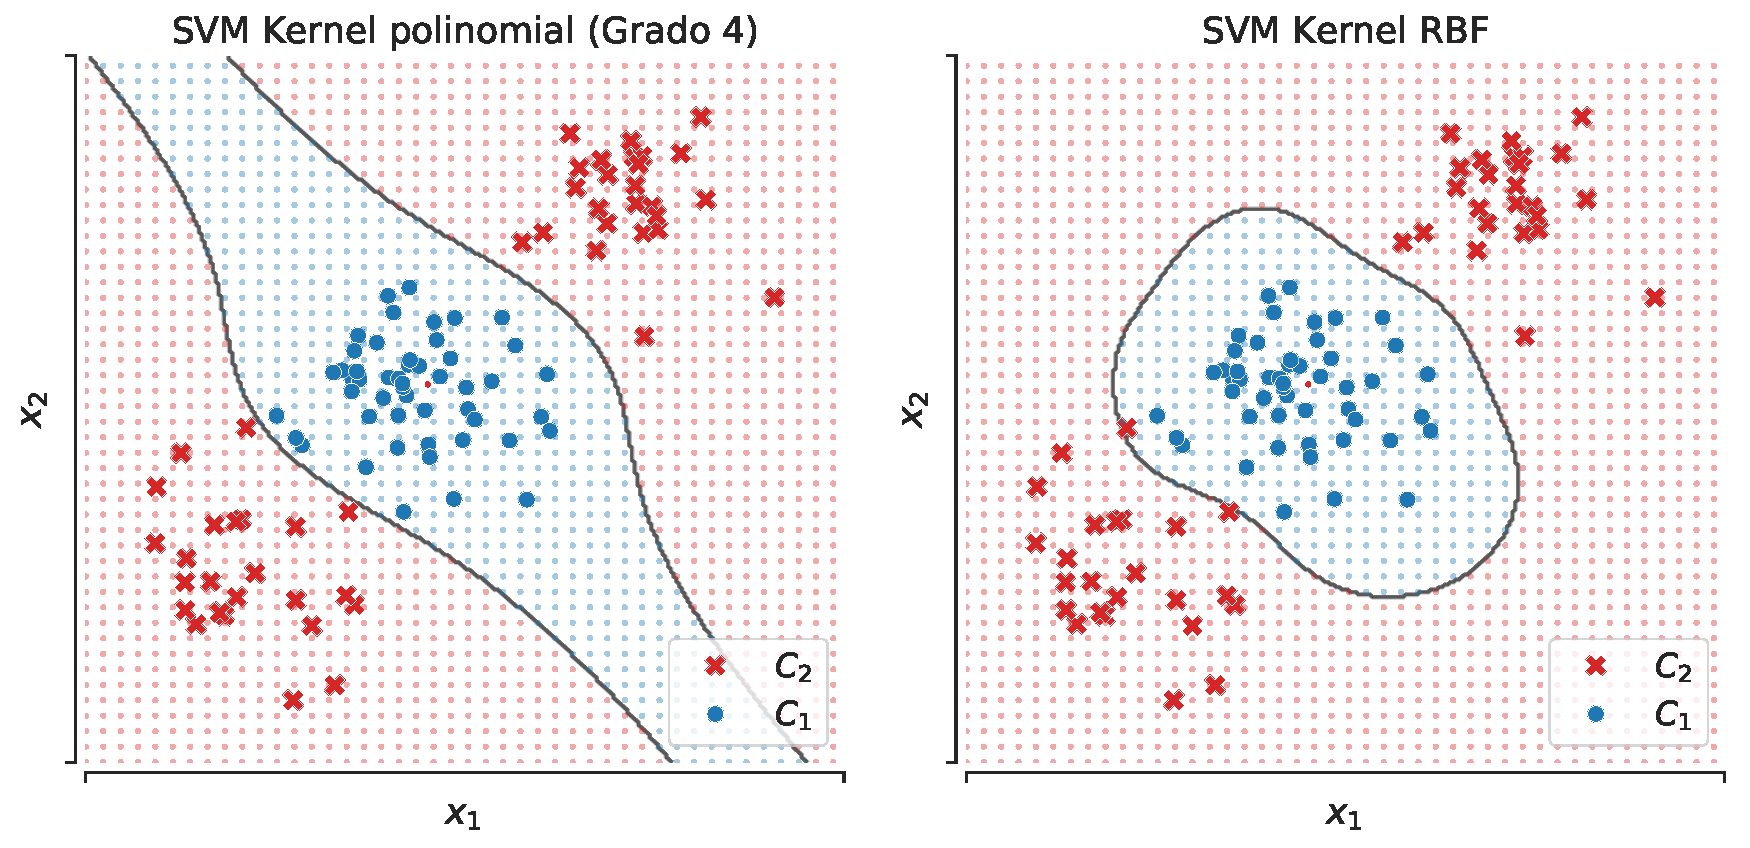
\includegraphics[width=0.8\textwidth]{img/cap5_svm_2kernels}
    \caption{Clasificación con distinto kernels.}
    \label{im:ca5_im6}
\end{figure}

A la izquierda se ocupo un kernel polinomial de grado $3$, dicho kernel permite un poco mas de curvatura en los límites del clasificador. A la derecha se ocupó un kernel RBF, el cual es capaz de encontrar fronteras de decisión más curvadas (Pero infinitamente diferenciables). 

Tener en cuenta que esta manera de resolver el problema tiene una tremenda ventaja computacional. Mover los datos a un espacio más grande mediante explícitamente definiendo $\phi(x)$, puede ser muy costoso, o incluso imposible en el caso que el espacio de llegada sea infinitamente dimensional. Usando funciones kernel dicha función queda implícita en el problema, dejandonos incluso trabajar en el caso infinito-dimensional (En el caso de RBF por ejemplo)


%-Comparar rendimiento de logistic regression c on SVM lineal
%-Usar diferentes Kernels
%-Ver el overfitting cuando ocupas un polinomio de muchos grados
%-Ver la importancia de escalar los datos


\newpage
%!TEX root = notas_de_clase.tex


\newcommand{\gp}{\ensuremath{\mathcal{GP}}}
\newcommand{\pr}{\ensuremath{\mathbb{P}}}
\newcommand{\x}{\ensuremath{\mathbf{x}}}
\newcommand{\y}{\ensuremath{\mathbf{y}}}
\newcommand{\bx}{\ensuremath{\textcolor{blue}{X}}}
\newcommand{\by}{\ensuremath{\textcolor{blue}{Y}}}
\newcommand{\rx}{\ensuremath{\textcolor{red}{X_*}}}


\newpage
\section{Procesos Gaussianos}


Como se vio en capítulos anteriores, el problema de regresión busca encontrar una función $y= f(x)$, dado un conjunto de pares de la forma $\mathcal{D}=\{(x_i, y_i)\}_{i=1}^N$. Dento de los métodos vistos para resolver el problema de regresión, se vio el de regresión lineal, lineal en los parámetros y no lineals. Una característica en común que tienen estos métodos es que el proceso de entrenamiento consiste en encontrar un número \textbf{fijo} de parámetros, que minimicen cierta función objetivo, donde la cantidad de parámetros y la forma del modelo es parte del diseño. A este tipo de modelos se les llama \textit{paramétricos}.\\

En contraste, se encuentran los modelos \textit{no paramétricos} los cuales \textbf{no} tienen un número fijo de parámetros, donde pueden llegar a ser en algunos casos infinito. Un ejemplo es el algoritmo k-vecinos más cercanos (KNN), donde los puntos del conjunto de entrenamiento son usados para clasificar nuevas muestras. Otro ejemplo son las máquinas de soporte vectorial (SVM) donde al entrenar se obtienen los vectores de soporte.\\

Es importante hacer la distinción entre parámetros que se aprenden y los parámetros de modelo, muchas veces llamados hyperparámetros, donde estos últimos pueden ser fijos independiente si el método es paramétrico y no paramétrico; esto se ve en el caso de SVM donde los parámetros serían los vectores de soporte, y los hyperparámetros serían el tipo de kernel, los parámetros de dicho kernel y los demás valores elegidos de antemano que definen el tipo de modelo.\\

En este capítulo introduciremos un método no paramétrico probabilístico de regresión no lineal, llamados Procesos Gaussianos ($\gp$), este en vez de encontrar un candidato único de la función a estimar, define una distribución sobre funciones $\mathbb{P}(f)$, donde $f(\cdot)$ es una función de un espacio de entrada $\mathcal{X}$ a los reales, $f: \mathcal{X} \rightarrow \mathbb{R}$. Esto tiene la virtud que permitirá cuantificar la incertidumbre puntual que existe en la predicción de nuestro modelo que servirá en forma de intervalos de confianza para la distribución Gaussiana.\\

Partiremos definiendo un $\gp$ como una distribución a priori sobre funciones, y mostraremos que la densidad posterior se puede encontrar de forma exacta y que esta también es un $\gp$, conservando sus propiedades.

\begin{equation}
	\mathbb{P}(f|\mathcal{D}) =  \frac{\pr(f)\pr(\mathcal{D}|f)}{\pr(\mathcal{D})}
\end{equation}

Es de notar que si $\mathcal{X}$ tiene cardinalidad infinita (por ejemplo $\mathcal{X}=\mathbb{R}$), $f(\cdot)$ puede ser visto como un vector infinito dimensional. Como en la práctica no podemos trabajar con un vector infinito dimensional, dados $n$ puntos $\{ x_i\}_{1}^{n}  \subset \mathcal{X}$ podemos definirnos el vector n-dimensional de valores de la funciones evaluados en dichos puntos $f(\mathbf{x})=[f(x_1), \ldots, f(x_n)]$.\\


\ovalbox{\textbf{Definición}:} Un Proceso Gaussiano ($\gp$) es una colección de variables aleatorias, tal que para cualquier subconjunto finito de puntos, estos tienen una distribución conjuntamente Gaussiana.\\ 

Al aplicar esta definición a nuestro caso anterior, $\pr(f)$ será un $\gp$ y para cualquier conjunto finito $\{ x_i\}_{1}^{n}  \subset \mathcal{X}$, la distribución de $\pr(f(\mathbf{x}))$ es Gaussiana multivariada $f(\mathbf{x})=[f(x_1), \ldots, f(x_n)]$). En este caso las variables aleatorias representan el valor de la función $f(x_i)$ en la posición $x_i$.\\


Un $\gp$ queda completamente caracterizado por su función de media $m(\cdot)$ y función de covarianza $K(\cdot, \cdot)$, de esta forma para cualquier conjunto finito podemos encontrar la distribución. Definimos estas funciones como

\begin{align}
	m(x) & = \mathbb{E}\left\{f(x)\right\}\\
	K(x, x') & = \mathbb{E}\left\{\left(f(x) - m(x)\right) \left(f(x') - m(x') \right)\right\}
\end{align}

Y de esta forma podemos escribir el proceso como:

\begin{equation}
	f \sim \gp(m(\cdot), K(\cdot, \cdot))
\end{equation}

Donde para un conjunto finito tenemos que la marginal resulta de la forma:

\begin{equation}
	f(\x) \sim \mathcal{N}(m(\x), K(\x, \x))
\end{equation}

Hasta el momento hemos hablado del espacio de entrada $\mathcal{X}$ como genérico, un caso común es definir los $\gp$ sobre el tiempo ($\mathbb{R}^{+}$), es decir que los $x_i$ son instantes de tiempo. Es de notar que este no es el único caso, y se podría definir sobre un espacio más general, por ejemplo $\mathbb{R}^d$.\\

Otro punto a notar es que como estamos hablando de una colección (no necesariamente finita) de variables aleatorias, es necesario que se cumpla la propiedad de marginalización (o llamada consistencia\footnote{Para más detalles puede ver el teorema de consistencia de Kolmogorov}). Esta propiedad se refiere a que si un $\gp$ define una distribución multivariada para digamos dos variables $(y_1, y_2) \sim \mathcal{N}(\mu, \Sigma)$ entonces también debe definir $y_1 \sim \mathcal{N}(\mu_1, \Sigma_{11})$ donde $\mu_1$ es la componente respectiva del vector $\mu$ y $\Sigma_{11}$ la submatriz correspondiente de $\Sigma$. En otras palabras, el tomar un subconjunto más grande de puntos no cambia la distribución de un subconjunto más pequeño. Y podemos notar que esta condición se cumple si tomamos la función de covarianza definida anteriormente.\\



\subsection{Muestreo de un prior $\gp$}

Como fue mencionado, un $\gp$ define un \textit{prior} sobre funciones, por lo que, antes de ver ningún dato se podría obtener una muestra de este proceso dado una función de media y covarianza. Un supuesto común es asumir la función de media $m(\cdot)=0$ por lo que solo nos queda definir una función de covarianza o kernel, un ejemplo de kernel es el \textit{Exponencial Cuadrático} (Square Exponential), también conocido como RBF (Radial Basis function) o Kernel Gaussiano (en general se evita este nombre porque este kernel no tiene relación con la distribución de los datos).

\begin{equation}
	K_{SE}(x, x') = \sigma^2 \exp\left( - \frac{\left( x- x'\right)^2}{2\ell^2} \right)
\end{equation}

Donde en este caso los parámetros son interpretables (y como veremos más adelante pueden ser aprendidos a través de un conjunto de entrenamiento) donde $\sigma^2$ es la varianza de la función, notar que esta es la diagonal de la matriz covarianza. El parámetro $\ell$ es conocido como el \textit{lenghtscale} que determina que tan lejos tiene influencia un punto sobre otro, donde en general un punto no tendrá influencia más allá de $\ell$ unidades alrededor.\\

Como sabemos, las funciones definidas por el $\gp$ son vectores infinito dimensionales, por lo que no podemos muestrear de toda la función, pero tomando una cantidad suficiente de puntos podemos graficar muestras de un $\gp$ dada una función de covarianza. Tomando un $\gp$ con media cero ($m(\cdot)=0$) y kernel SE, muestras del proceso para distintos valores de $\ell$ obtenemos la Fig.\ref{fig:gp_1}, donde el área sombreada corresponde al intervalo de confianza del $95\%$. Se puede ver que el parámetro $\ell$ controla que tan erráticas son las funciones, donde a medida que va a aumentando las muestras se vuelven funciones más suaves.

\begin{figure}[H]
	\centering
	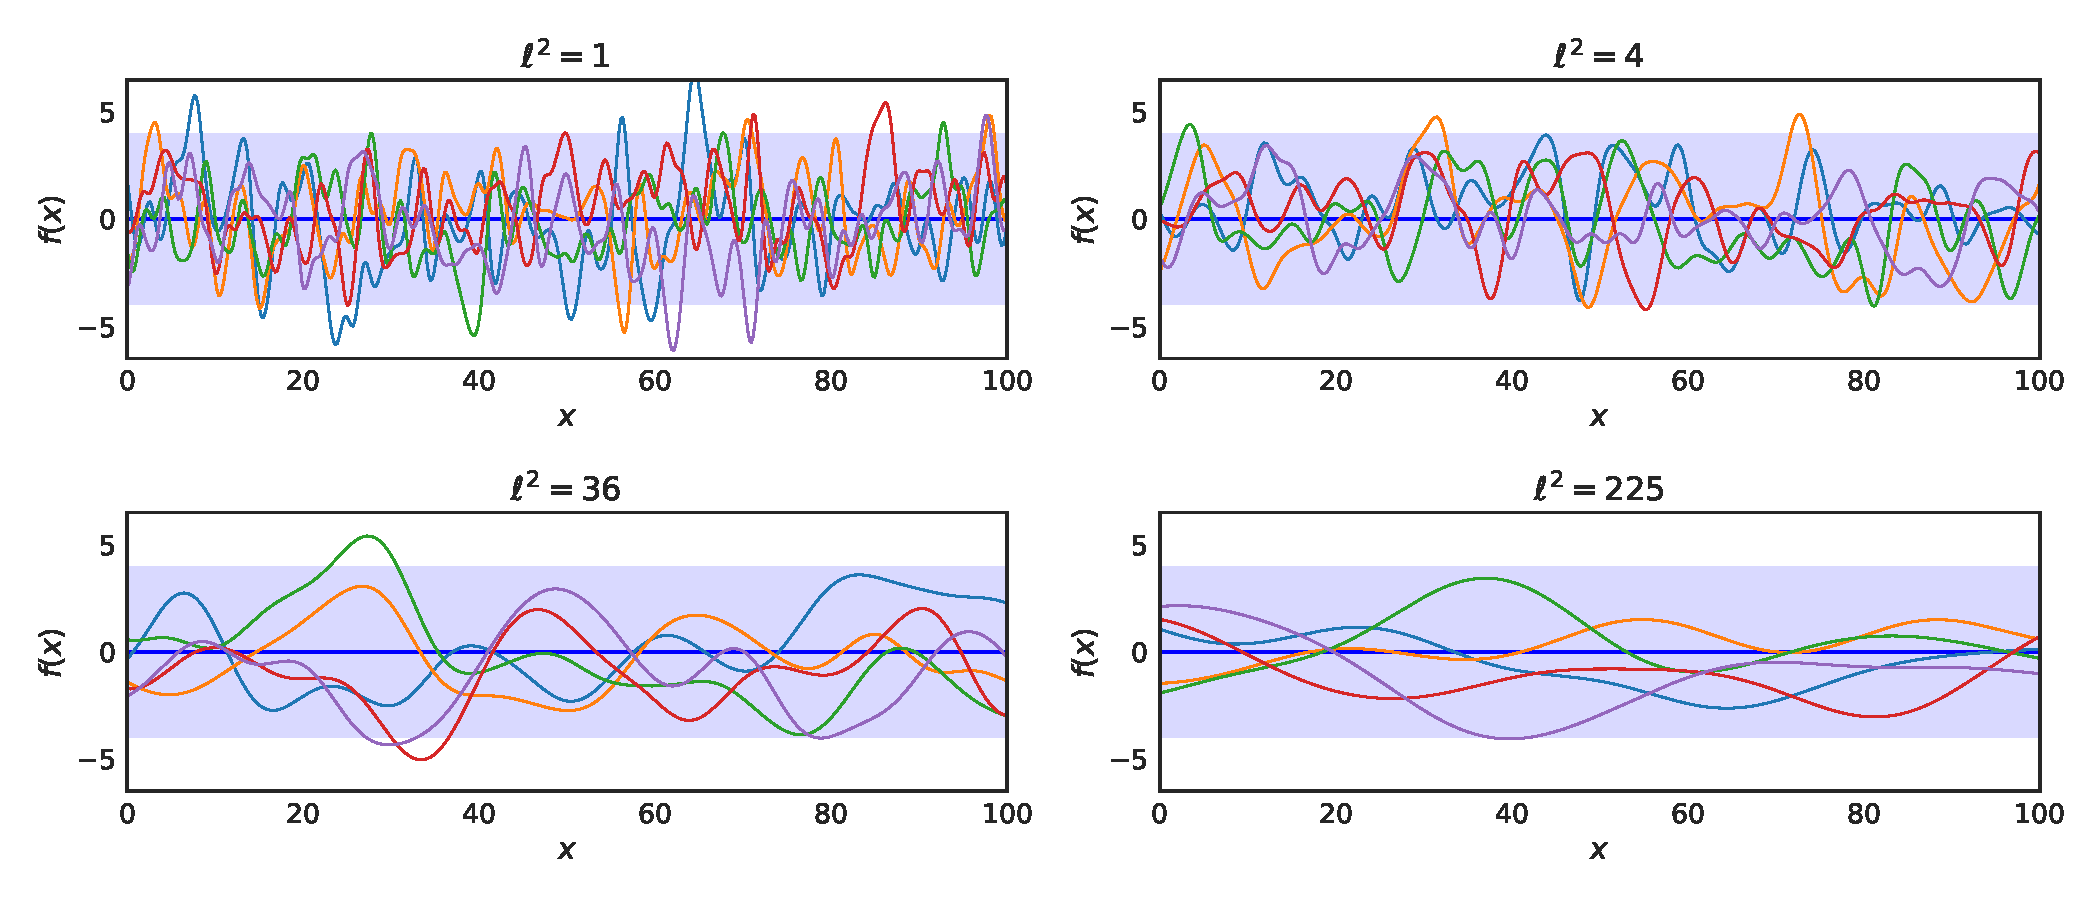
\includegraphics[width=0.9\textwidth]{img/gp_prior_samples.pdf}
	\caption{Muestras de un prior $\gp$ con kernel SE, para distintos \textit{lenghtscales} ($\ell$) y función media $m(\cdot)=0$, la parte sombreada corresponde al intervalo de confianza del $95\%$. Se puede ver que a mayor $\ell$ las funciones se van volviendo más suaves.}
	\label{fig:gp_1}
\end{figure}

\subsection{Incorporando Información: Evaluación sin ruido}

Ahora que ya podemos muestrear de nuestro prior, nos interesaría incorporar las observaciones que tenemos de la función a nuestro modelo. Para esto, primero consideramos el caso en que las observaciones son sin ruido, es decir tenemos observaciones de la forma $\{x_i, f(x_i)\}_{1}^{n}$, donde tenemos el valor real de nuestra función en los puntos $[x_1, \ldots, x_n]=\bx$. 

Luego, tenemos el par de entradas y observaciones $\left(\textcolor{blue}{X}, f(\textcolor{blue}{X})\right)$ digamos que queremos realizar una predicción en el conjunto $\textcolor{red}{X_*}$ de $n_*$ puntos, luego la distribución conjunta es de la forma:

\begin{align}
	\begin{bmatrix} f(\bx) \\ f(\rx)  \end{bmatrix}
	\sim \mathcal{N} \left(
	\begin{bmatrix} m(\bx) \\ m(\rx)  \end{bmatrix}, 
	\begin{bmatrix}
		K(\bx, \bx) & K(\bx, \rx) \\ K(\rx, \bx) & K(\rx, \rx)
	\end{bmatrix}
	 \right)
\end{align}

Donde la submatriz $K(\bx, \rx)$ es de $n \times n_*$, $K(\bx, \bx)$ de $n \times n$ y así respectivamente para cada submatriz.

Pero a nosotros nos interesa encontrar la densidad posterior de $f(\cdot)$, y dada las observaciones y una función de covarianza podemos evaluar la verosimilitud, que también es Gaussiana, lo que nos lleva a un punto clave de los Processos Gaussianos.\\

\doublebox{
\begin{minipage}{.95\linewidth}
\textbf{Dado un prior $\gp$ sobre $f(\cdot)$ y una verosimilitud Gaussiana, la posterior sobre $f(\cdot)$ es también un $\gp$.}
\end{minipage}}\\

Luego, podemos condicionar sobre las observaciones $(\bx, f(\bx))$ y obtenemos

\begin{align}
	& f(\rx)|f(\bx), \bx  \sim \mathcal{N}(m_{\rx|\bx}, \Sigma_{\rx|\bx})\\ \label{eq:gp_post}
	& \quad \text{Donde la media y covarianza son:} \nonumber \\
	m_{\rx|\bx} & = m(\rx) + K(\rx, \bx)K^{-1}(\bx, \bx) (f(\bx) - m(\bx))\\
	 \Sigma_{\rx|\bx} & = K(\rx, \rx) - K(\rx, \bx)K^{-1}(\bx, \bx) K(\bx, \rx)
\end{align}


Ahora, dado un conjunto de observaciones y dada una función de covarianza, podemos obtener la densidad posterior. Para mostrar esto tomemos el caso de hacer regresión para una función conocida, para la cual tenemos observaciones sin ruido muestreadas no uniformemente, con estas observaciones queremos encontrar la función real de las que provienen; para esto usamos un prior $\gp$ con función media nula y kernel SE (por el momento tendrá parámetros fijos), nos damos un rango donde queremos hacer predicción y condicionamos en las observaciones usando la Ec.(\ref{eq:gp_post}). En este caso las observaciones corresponden al 15$\%$ de los puntos generados por nuestra función sintética.\\

Esto se muestra en la Fig.\ref{fig:gp_2}, donde podemos ver que la media de la posterior pasa por las observaciones sin incertidumbre asociada, es decir que para estos puntos se tiene una posterior degenerada pues no hay varianza. Se puede ver que a medida que la predicción se aleja de las observaciones el intervalo de confianza (al que lo podemos asociar con incertidumbre del modelo) va creciendo.

\begin{figure}[H]
	\centering
	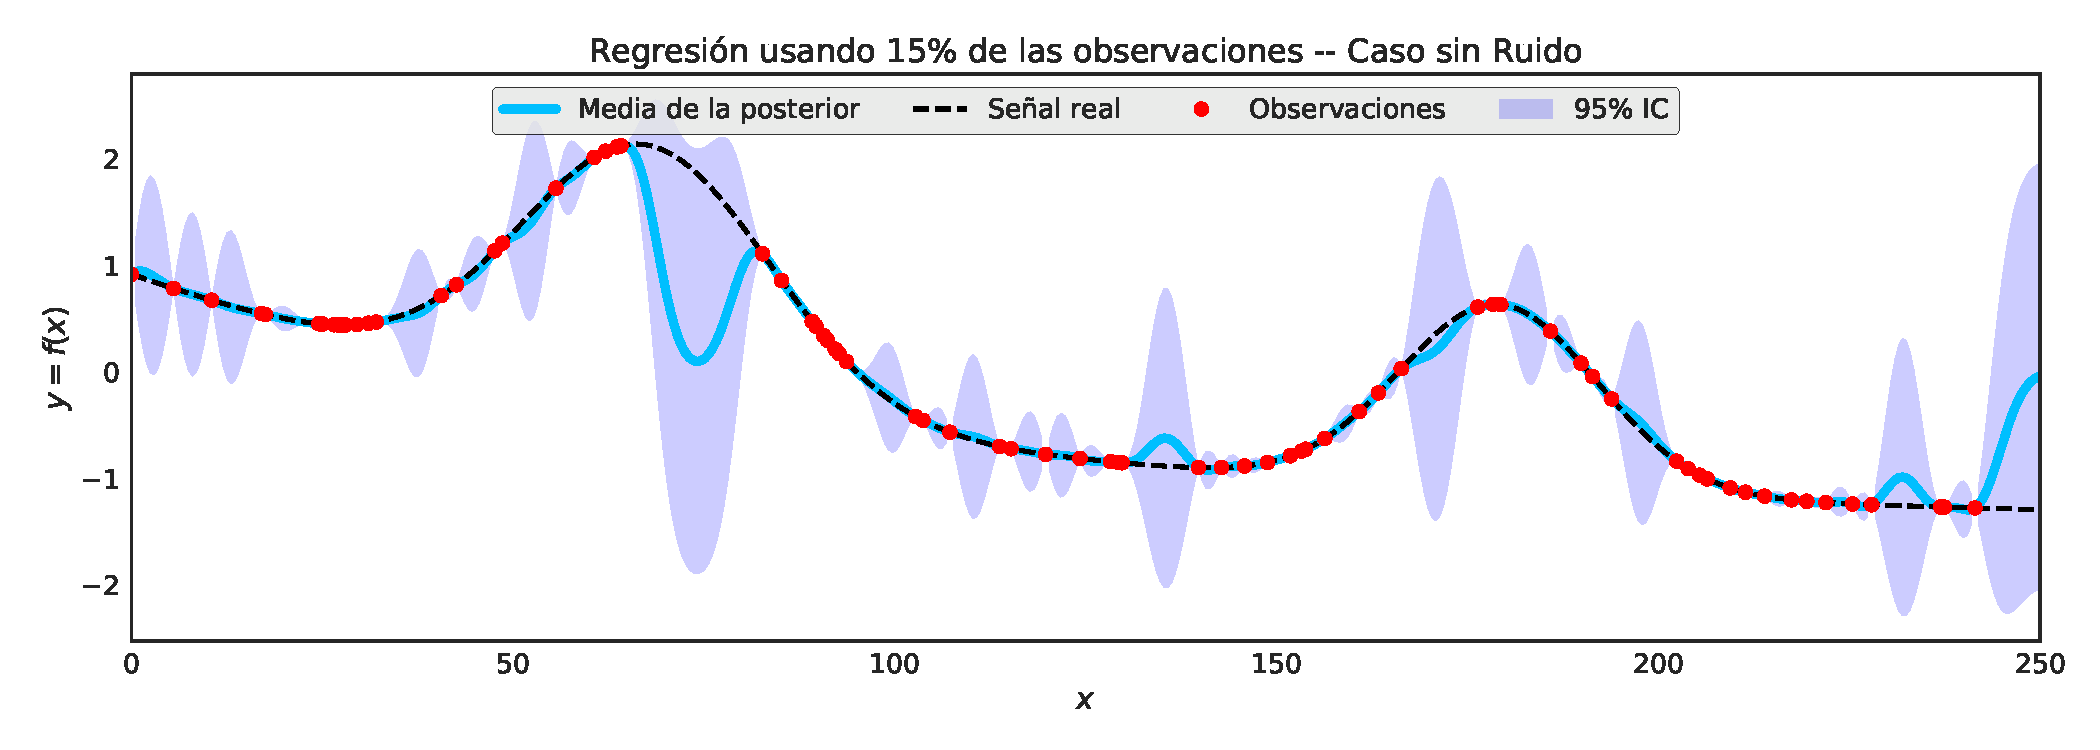
\includegraphics[width=0.9\textwidth]{img/gp_posterior_noiseless.pdf}
	\caption{Regresión con $\gp$ para señal sintetica usando el 15$\%$ de los datos muestreados de forma no uniforme, utilizand un $\gp$ de media nula y kernel SE.} 
	\label{fig:gp_2}
\end{figure}

\subsection{Incorporando Información: Evaluación con ruido}

En aplicaciones reales el caso de tener observaciones sin ruido es poco habitual, por lo que si queremos incorporar la incertidumbre real debemos tomar en cuenta errores de medición en nuestro modelo. Tomemos el caso de tener observaciones contaminadas con ruido i.i.d (independientes idénticamente distribuidas) donde las observaciones serán de la forma $y_i = f(x_i) + \eta$ donde $\eta \sim \mathcal{N}(0, \sigma_n^2)$, donde ahora nuestro conjunto de observaciones es de la forma $(\bx, \by)$ donde $\by=f(\bx) + \eta$.

Lo que en nuestro modelo equivale a agregar un término a la función de covarianza

\begin{equation}
	cov(\by) = K(X, X) + \sigma_n^2\eye
\end{equation}

Donde si tenemos el mismo caso anterior, observaciones $(\bx, \by)$ y queremos evaluar en $\rx$, la conjunta queda


\begin{align}
	\begin{bmatrix} \by \\ f(\rx)  \end{bmatrix}
	\sim \mathcal{N} \left(
	\begin{bmatrix} m(\bx) \\ m(\rx)  \end{bmatrix}, 
	\begin{bmatrix}
		K(\bx, \bx) + \sigma_n^2 \eye & K(\bx, \rx) \\ K(\rx, \bx) & K(\rx, \rx)
	\end{bmatrix}
	 \right)
\end{align}

Notemos que el termino de ruido solo es agregado al subbloque correspondiente a las observaciones, no se agrega el termino en los otros subbloques pues buscamos hacer una predicción de la función latente $f(\cdot)$ y no una versión ruidosa de esta.
Igual que en el caso sin ruido, podemos condicionar esta conjunta a las observaciones y obtenemos

\begin{align}
	& f(\rx)|\by, \bx  \sim \mathcal{N}(m_{\rx|\bx}, \Sigma_{\rx|\bx})\\ \label{eq:gp_posterior}
	& \quad \text{Donde la media y covarianza son:} \nonumber \\
	m_{\rx|\bx} & = m(\rx) + K(\rx, \bx) [K(\bx, \bx) + \sigma_n^2 \eye]^{-1} (\by - m(\bx))\\
	 \Sigma_{\rx|\bx} & = K(\rx, \rx) - K(\rx, \bx) [K(\bx, \bx) + \sigma_n^2 \eye]^{-1} K(\bx, \rx)
\end{align}


Si tomamos el mismo ejemplo anterior, pero añadimos el ruido al modelo, obtenemos la predicción de la Fig.\ref{fig:gp_3}. En este caso podemos ver que la media de la posterior no necesariamente coincide su valor con el de la observación, pues se toma en cuenta la incertidumbre en las observaciones mismas, también se ve que no se obtienen soluciones degeneradas incluso en zonas donde hay observaciones aglomeradas.


\begin{figure}[H]
	\centering
	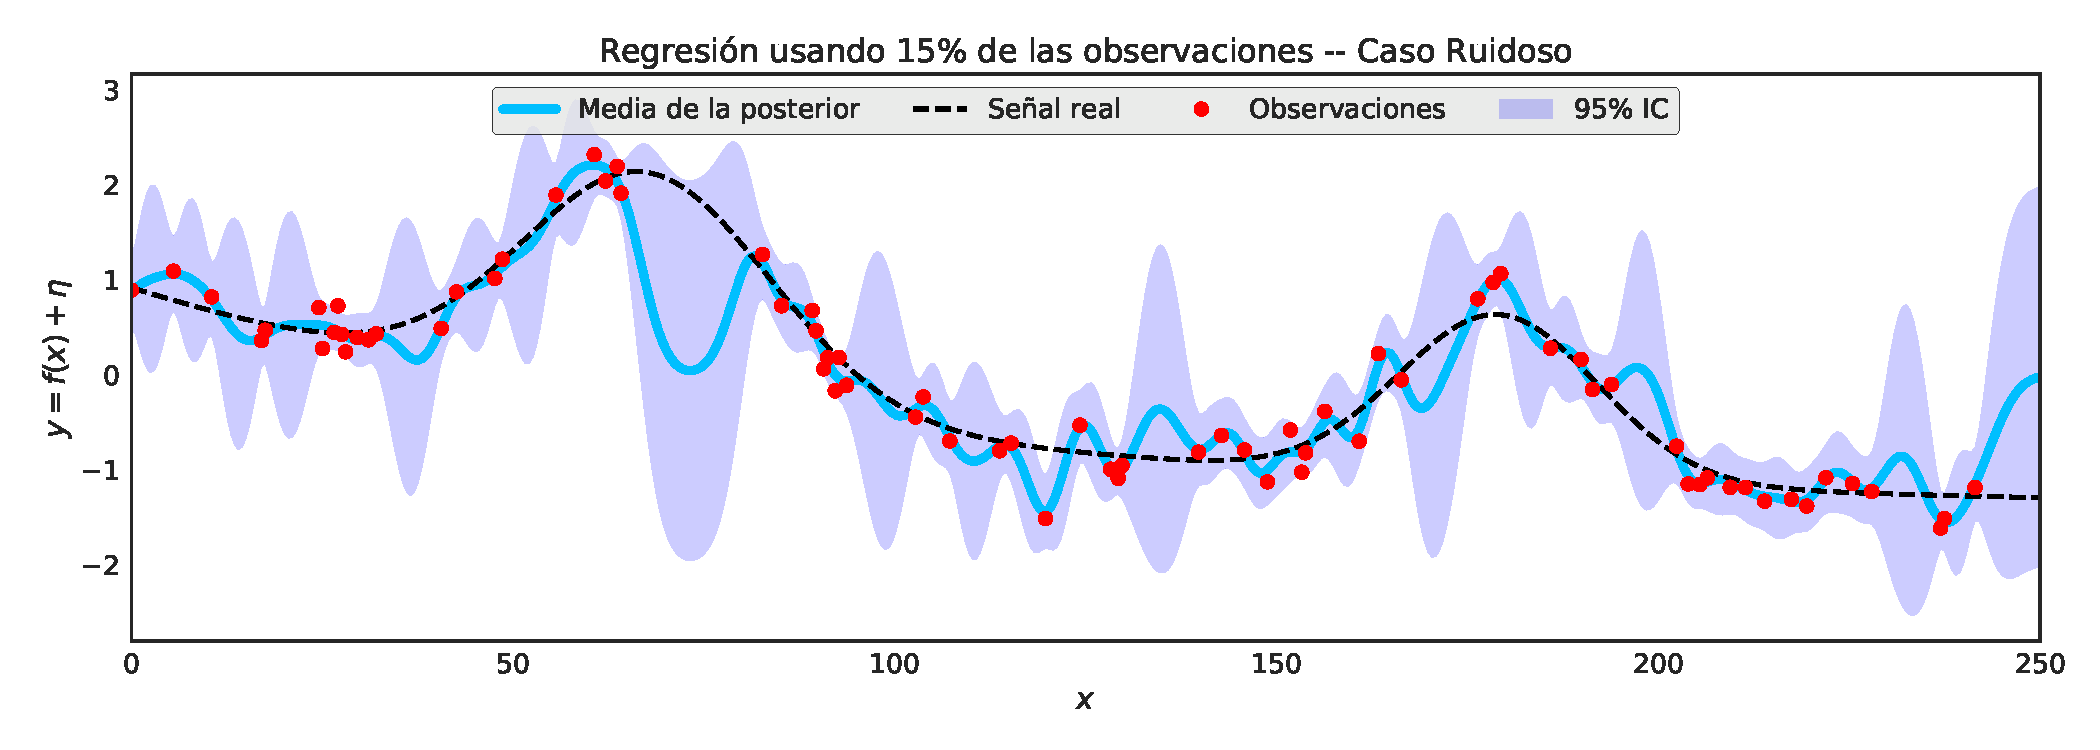
\includegraphics[width=0.9\textwidth]{img/gp_posterior_noisy.pdf}
	\caption{Regresión con $\gp$ para señal sintetica usando el 15$\%$ de los datos muestreados de forma no uniforme y contaminados con ruido Gaussiano, utilizando un $\gp$ de media nula y kernel SE.}
	\label{fig:gp_3}
\end{figure}



\subsection{Entrenamiento y optimización de un $\gp$}

hasta el momento nos hemos dado la función de covarianza y sus parámetros, por lo que aún no hemos hecho realizado el \textit{aprendizaje} de nuestro $\gp$, que es lo que haremos a continuación.\\

\noindent{\textbf{¿Qué es entrenar un $\gp$?}}

Vimos que dada una función de covarianza podemos representar el proceso, y podemos encontrar analíticamente la densidad posterior de nuestra función $f(\cdot)$ condicionando a las observaciones. Pero la forma que tendrá la posterior y la función fuera de las observaciones dependerá fuertemente en nuestra función kernel escogida, en este sentido, para un kernel dado nos gustaría encontrar los parámetros de este que mejor representen nuestra función a estimar.\\

Nos referiremos a entrenar u optimizar un $\gp$ cuando queremos obtener los hyperparámetros, es decir los parámetros del kernel (los denotamos $\theta$) y la varianza del ruido (la denotamos $\sigma_n^2$) si es que aplica.

Para esto nos gustaría poder comparar funciones de covarianza, o mejor aún un funcional que podamos optimizar, afortunadamente podemos usar la \textit{verosimilitud marginal}, obtenida marginalizando sobre la función $f(\cdot)$, donde dado un conjunto de entrenamiento $(X, Y)= \{(x_i, y_i)\}_{i=1}^{n}$, esta dada por

\begin{align}
	\pr(Y|X, \theta, \sigma) & = \int \pr(Y|f, X, \theta, \sigma_n) p(f|X,\theta, \sigma) df \\
	& = \frac{1}{\left( 2\pi |\mathbf{K}_y|\right)^{\frac{n}{2}}} 
	\exp \left(
	-\frac{1}{2} (Y - \mathbf{m})^T \mathbf{K}_y^{-1} (Y - \mathbf{m})
	\right)
\end{align}

Donde $\mathbf{m}=m(X)$ y $\mathbf{K}_y=K_{\theta}(X,X) + \sigma_n^2 \eye$, la matriz de covarianza dados los parámetros $\theta$ agregando el término de la diagonal correspondiente al ruido. De la misma forma que lo hacemos con otros modelos probabilísticos, en vez de maximizar la verosimilitud, en conveniente minimizar la log-verosimilitud negativa (NLL) dada por la expresión:

\begin{align}
	NLL & = -\log \pr(Y|X, \theta, \sigma_n) \\
	NLL & = \textcolor{blue}{\underbrace{ \color{black}{\frac{1}{2}\log|\mathbf{K_y}|} }_
	    {\text{\parbox{2cm}{\centering Penalización\\[-4pt] por\\[-4pt] complejidad}}}}
	    + \textcolor{Green}{\underbrace{ \color{black}{\frac{1}{2}(Y - \mathbf{m})^T \mathbf{K}_y^{-1} (Y - \mathbf{m}) }}_
	    {\text{\parbox{4cm}{\centering Data fit (Única parte que depende de $Y$)}}}}
	    + \textcolor{red}{\underbrace{ \color{black}{\frac{n}{2} \log2\pi}}_
	    {\text{\parbox{2cm}{\centering Constante de normalización}}}} \label{eq:gp_nll}
\end{align}

De izquierda a derecha, el primer término tiene el rol de penalizar por la complejidad del modelo, y vemos que depende solo del kernel y las entradas; el segundo término cuantifica que tan bien se ajusta el modelo a los datos, y es la única componente que depende de las observaciones $Y$ (ruidosas) de la función, el último término es una constante de normalización.\\



\begin{wrapfigure}{r}{0.42\textwidth}
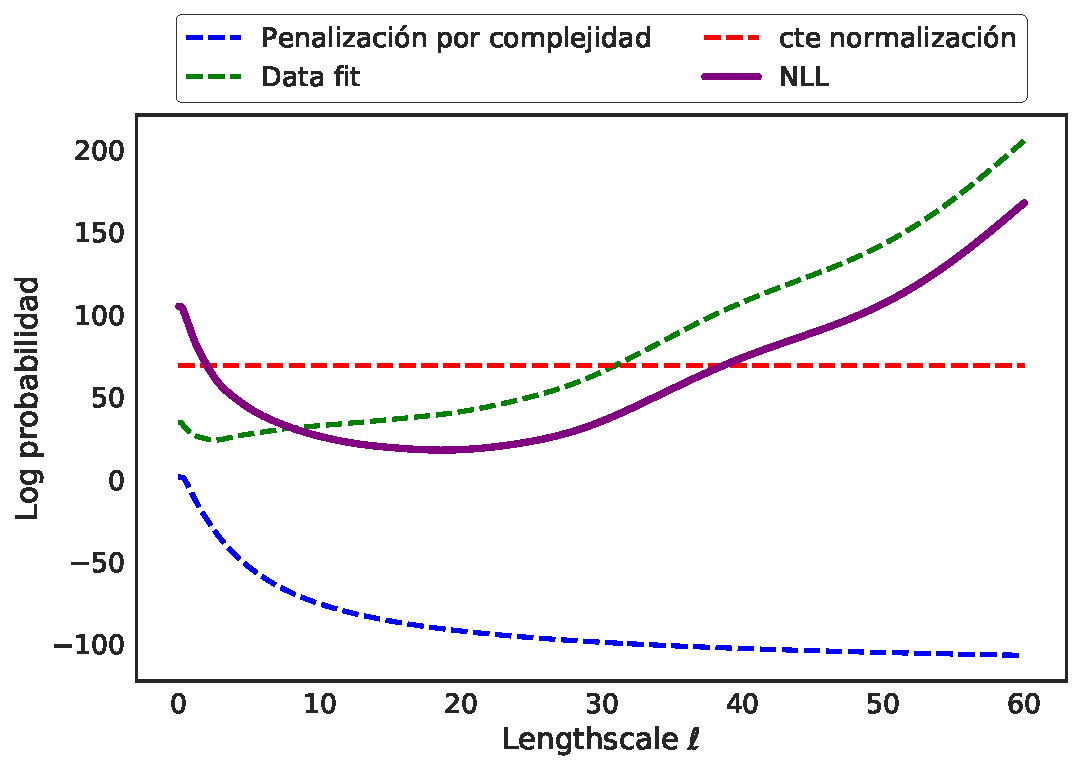
\includegraphics[width=0.42\textwidth]{img/gp_nll_divided.pdf}
\caption{Log verosimilitud marginal negativa (NLL) en función del \textit{lengthscale} ($\ell$) para señal sintetica, se mantienen constantes los otros parámetros del $\gp$.}\label{fig:gp_4}
\end{wrapfigure} 

Siguiendo con los ejemplos anteriores, para el mismo conjunto de observaciones ruidosas, se calculan las tres componentes de la $NLL$, utilizando un kernel SE, para este caso, se dejan fijo tanto la varianza de la señal como la varianza del ruido y se varia el \textit{lengthscale} $\ell$ del kernel, en la Fig.\ref{fig:gp_4}.

Al ir variando $\ell$ se ve que la penalización por complejidad va disminuyendo, pues a mayor $\ell$ menos complejas son las funciones (recordar Fig.\ref{fig:gp_1}, a mayor $\ell$ más suaves y regulares las muestras), también vemos que la componente del ajuste de datos comienza a decaer y luego se mantiene en incremento, pues a mayor \textit{lengthscale} el modelo se vuelve menos flexible, por lo que no es capaz de ajustarse de manera correcta a los datos. De esta forma, el proceso de entrenamiento dará preferencia a funciones que se ajusten bien a los datos sin ser tan complejas, ahora viendo el valor total del NLL vemos que este alcanza su mínimo en $\ell$ en el rango de $[10-30]$.\\


Ya tenemos una noción de que es entrenar un $\gp$, queremos minimizar la $NLL$ (Ec.(\ref{eq:gp_nll})) y encontrar los parámetros del kernel y del ruido (si aplica). Ahora discutiremos formas de optimizar este funcional.\\

\noindent{\textbf{¿Cómo se entrena?}}

Como contamos con una expresión cerrada para la NLL, podemos utilizar métodos clásicos de optimización, una opción es calcular el gradiente de esta función objetivo y aplicar algún método basado en gradiente, como L-BFGS; otra es utilizar el método de Powell que no requiere que la función sea diferenciable, por lo que no utiliza gradiente.\\
\\

Siguiendo ejemplos anteriores, usando la misma señal sintética y las mismas observaciones ruidosas de la Fig.\ref{fig:gp_3}, ahora optimizamos nuestro $\gp$ utilizando L-BFGS, lo que nos entrega como resultado el mostrado en la Tabla.\ref{tab:gp_1} donde comparamos los parámetros del $\gp$ sin entrenar usado en la Fig.\ref{fig:gp_3}, podemos ver que no difiere mucho en cuanto a las varianzas, pues como es una señal sintética poseíamos control sobre la varianza del ruido, el valor obtenido luego de optimizar es cercano al valor real (0.2), vemos que el \textit{lengthscale} óptimo es concordante con lo analizado en la Fig.\ref{fig:gp_4}.

Por último, podemos ver la predicción usando este $\gp$ optimizado en la Fig.\ref{fig:gp_5} donde vemos que se tiene una del proceso más concordante con la función real, esto se ve especialmente en la zona con pocas observaciones, entre 50 y 100 para $x$, donde el $\gp$ sin entrenar presentaba mucha incertidumbre en esa zona, en cuanto ahora se tiene un intervalo de confianza más bien limitado pues la señal no era muy compleja.

\begin{table}[H]
\centering
\begin{tabular}{lcccc}
 & $\sigma_{\text{ruido}}$ & $\ell$ & $\sigma_{\text{señal}}$ & NLL\\ \hline
Sin entrenar & 0.2 & 3.1622 & 1 & $\mathbf{55.3538}$\\
Entrenado & 0.2067 & 18.7267 & 0.9956 & $\mathbf{17.6945}$\\
\end{tabular}
\caption{Resultado optimización $\gp$ y comparación con los parámetros sin entrenar.}
\label{tab:gp_1}
\end{table}


\begin{figure}[H]
	\centering
	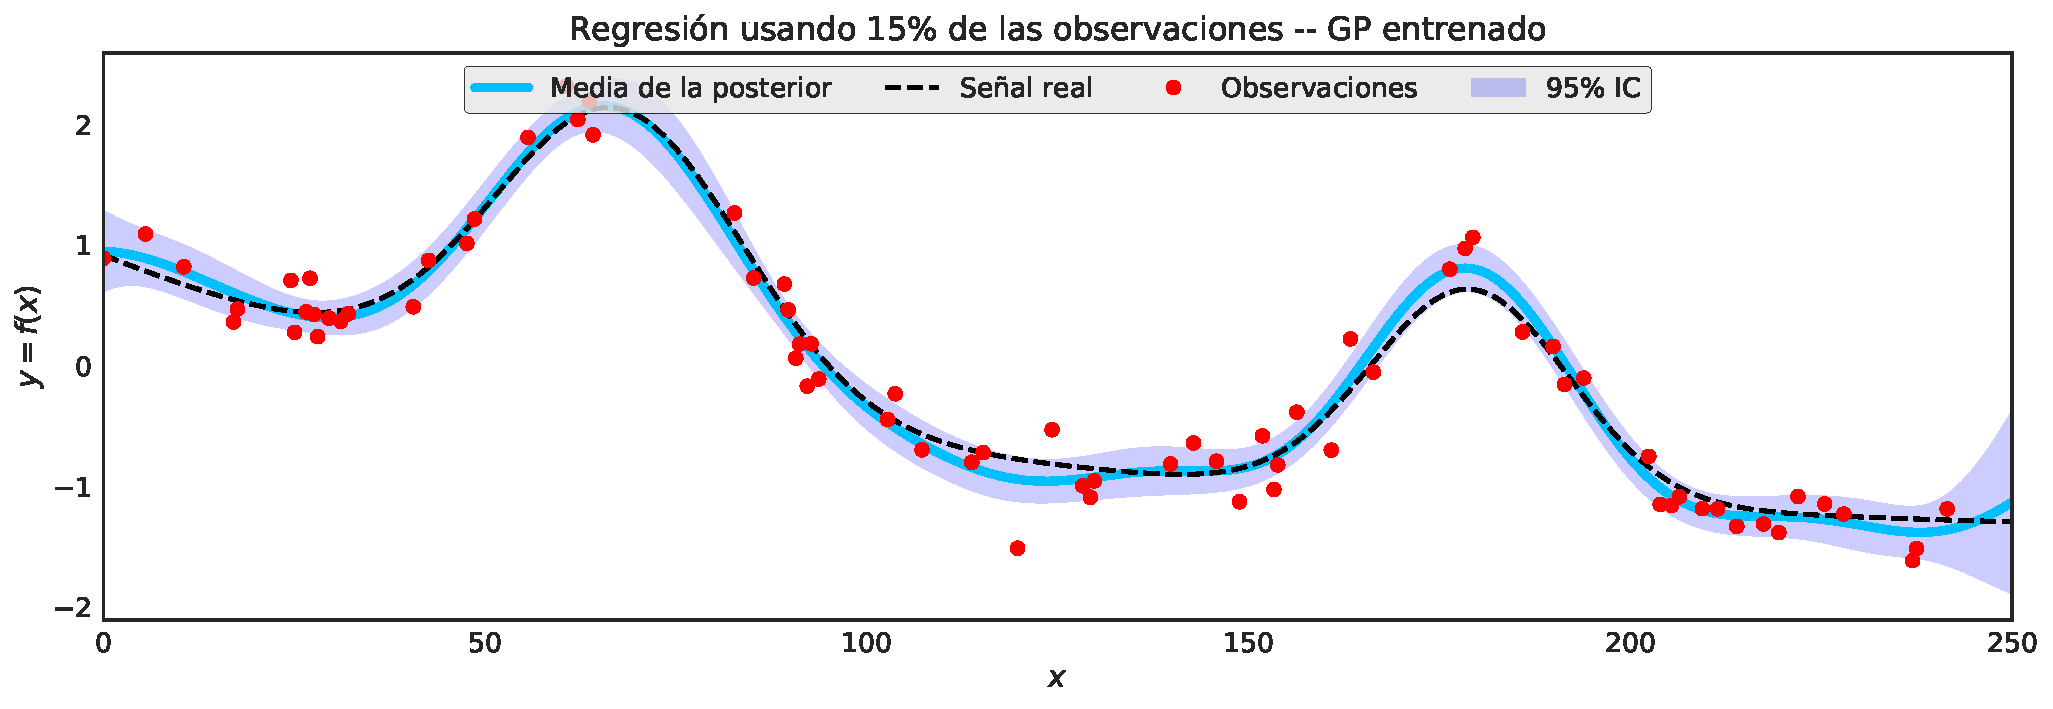
\includegraphics[width=0.9\textwidth]{img/gp_trained.pdf}
	\caption{Regresión con $\gp$ para señal sintetica usando el 15$\%$ de los datos muestreados de forma no uniforme y contaminados con ruido Gaussiano, utilizando un $\gp$ de media nula y kernel SE; Modelo optimizado utilizando L-BFGS.}
	\label{fig:gp_5}
\end{figure}

La desventaja de utilizar métodos tradicionales de optimización es que estos entregan una solución puntual (en el sentido de un valor para cada parámetro, el $\gp$ sigue siendo una distribución sobre funciones), en distintas aplicaciones puede que un valor fijo de parámetros no represente de manera idónea el proceso latente a estudiar. Una opción sería computar la densidad posterior de los parámetros del kernel condicionado a las observaciones. Lamentablemente en la mayoría de los casos no existe una expresión cerrada para esta posterior, por lo que debemos recurrir a métodos de \textit{inferencia aproximada} como Markov Chain Monte Carlo (MCMC) o Inferencia Variacional.




% \subsubsection{Métricas de evaluación}
% ---pendiente---

\subsubsection{Complejidad Computacional}

Es importante reconocer una de las principales desventajas de utilizar un $\gp$ cuando se cuenta con una gran cantidad de datos, esto es, su costo computacional.
Recordando, cuando queremos entrenar nuestro $\gp$ vamos a minimizar la log verosimilitud marginal negativa (NLL), mostrada en la Ec.(\ref{eq:gp_nll}), donde al observar en segundo término vemos que es la operación más costosa siendo $\mathcal{O}(n^3)$ con respecto al número de puntos de entrenamiento $n$. Hay que tomar en cuenta que la evaluación de la NLL se debe hacer en cada iteración del método de optimización elegido.

En cuanto a la evaluación, esta está dada por la Ec.(\ref{eq:gp_posterior}), donde en este caso vemos que es de orden cuadrático $\mathcal{O}(n^2)$ con respecto al número de puntos de test. Es de notar que esta vez no tomamos en cuenta la inversa de la matriz de Gram del conjunto de entrenamiento, pues puede ser precalculada y ser usada para múltiples conjuntos de test.\\

Lo anterior mencionado limita la cantidad de problemas que se pueden abordar usando estos procesos, sin embargo existen formas de obtener aproximaciones que siguen manteniendo la estructura y deseables propiedades de los $\gp$ a un menor costo computacional, estos reducen el orden de $\mathcal{O}(n^3)$ a $\mathcal{O}(nm^2)$ en entrenamiento y $\mathcal{O}(m^2)$ en test, con $m<n$. Un ejemplo de estos son los \textit{Sparse Gaussian Processes} que utilizan una aproximación de rango bajo para la matriz de covarianza, utilizando \textit{pseudo-inputs} en vez el conjunto de entrenamiento completo.


\subsection{Funciones de covarianza (Kernels)}

Una función de covarianza es una función de dos argumentos donde cualquier matriz que se obtiene como resultado en la evaluación de un conjunto de puntos (la llamaremos matriz de Gram) es semidefinida positiva.

Hasta el momento solo hemos utilizado un tipo de función de covarianza, el llamado kernel \textit{Squared Exponential} (SE), conocido también como kernel RBF, dado por la Ec.(\ref{eq:gp_kernel_se}). En esta sección mostraremos distintos tipos de funciones de covarianza y los distintos tipos de funciones que generan.

\begin{equation}\label{eq:gp_kernel_se}
	K_{SE}(x, x') = \sigma^2 \exp\left( - \frac{\left( x- x'\right)^2}{2\ell^2} \right)
\end{equation}

Es importante denotar tipos de familias de funciones de covarianza, si la función solo depende de la diferencia, es decir $k(x, x')=k(x-x')$ se le llamará \textit{kernel estacionario}, más aún, si depende solo de la norma de la diferencia $k(x, x')=k(|x-x'|)$ se le llamará \textit{kernel isométrico}, un ejemplo de esto es el kernel SE.\\

Es de notar que kernels estacionarios hacen que la covarianza entre puntos sea invariante a traslaciones en el espacio de entradas. Una noción importante es que un kernel puede ser visto como una medida de similaridad entre puntos, y en el caso de kernels estacionarios, mientras más cercanos estén dos puntos más símiles serán.\\

\textbf{Kernel \textit{Rational Quadratic} (RQ)}\\

Este kernel viene dado por la Ec.(\ref{eq:gp_kernel_rq}), este puede ser interpretado como una suma infinita de kernels SE con distintos \textit{lenghtscale}, donde $\alpha$ es un parámetro de variación de escala, notar que cuando $\alpha \rightarrow \infty$ el kernel tiende a uno SE. En la Fig.\ref{fig:gp_6} se muestra el kernel RQ, a la izquierda se ve el valor de la covarianza en función de la diferencia de los argumentos $x-x'$, a la derecha se muestran diferentes muestras de funciones con este kernel.
 
\begin{equation}\label{eq:gp_kernel_rq}
	K_{RQ}(x, x') = \sigma^2 \left(1 + \frac{\left( x- x'\right)^2}{2\alpha\ell^2 } \right)^{-\alpha}
\end{equation}


\begin{figure}[H]
	\centering
	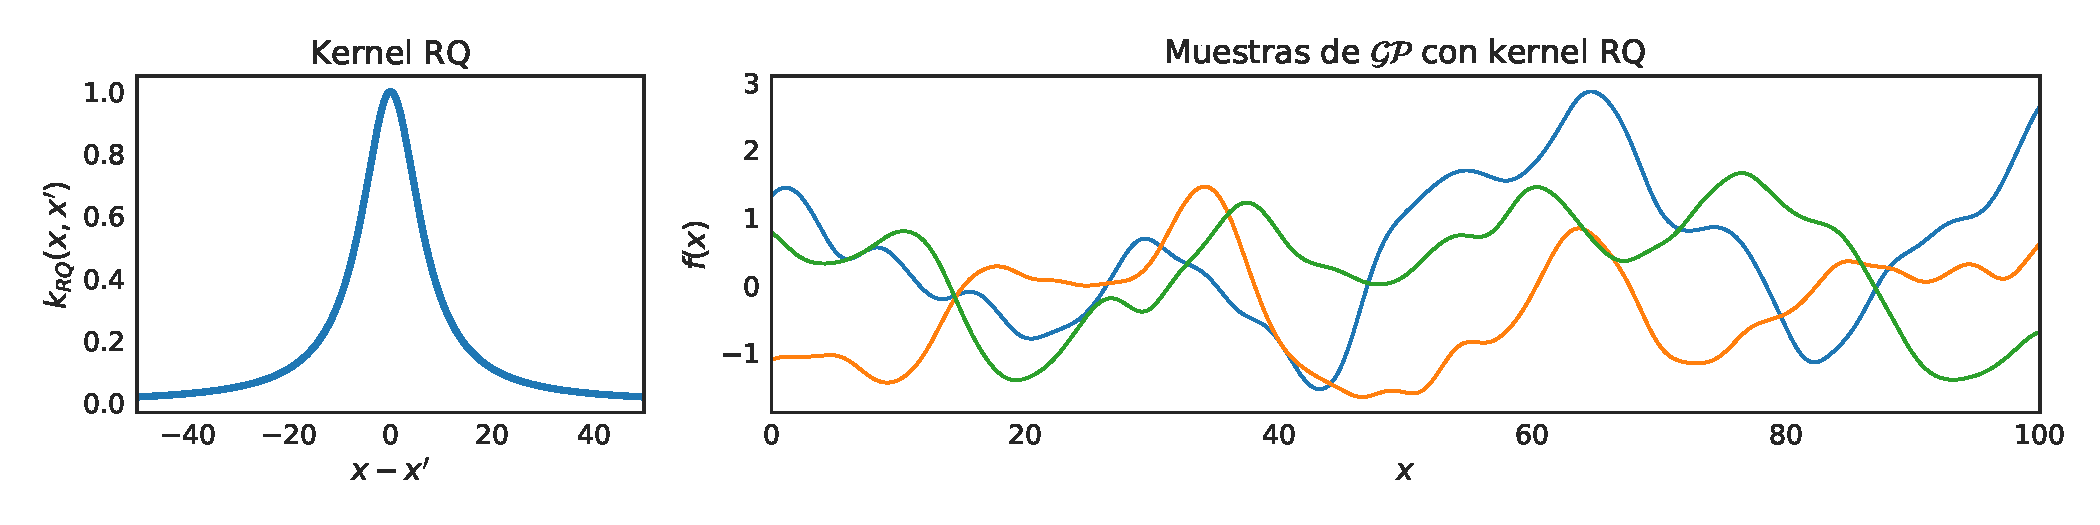
\includegraphics[width=0.9\textwidth]{img/gp_samples_RQ.pdf}
	\caption{Kernel \textit{Rational Quadratic}, en la izquierda se muestra la covarianza en función de su argumento $\tau=x-x'$, a la derecha de un $\gp$ usando un kernel RQ.}
	\label{fig:gp_6}
\end{figure}

\textbf{Kernel Periódico}\\

Como su nombre lo indica, este kernel, dado por la Ec.(\ref{eq:gp_kernel_p}), permite modelar funciones periódicas, donde el parámetro $p$ controla el periodo de la función. Una extensión de este el kernel localmente periódico, dado por la Ec.(\ref{eq:gp_kernel_lp}) que es un kernel SE ponderado por uno periódico, este da la libertad de tener funciones con una estructura periódica local.


\begin{equation}\label{eq:gp_kernel_p}
	K_{P}(x, x') = \sigma^2 \exp\left(-\frac{2\sin^2\left(\pi |x- x'| / p \right)}{\ell^2 } \right)
\end{equation}

\begin{equation}\label{eq:gp_kernel_lp}
	K_{LP}(x, x') = \sigma^2  \exp\left(-\frac{\left(x- x' \right)^2}{2\ell^2 } \right) \exp\left(-\frac{2\sin^2\left(\pi |x- x'| / p \right)}{\ell^2 } \right)
\end{equation}

En la Fig.\ref{fig:gp_7} se muestra el kernel periódico, a la izquierda se ve el valor de la covarianza en función de la diferencia de los argumentos $x-x'$, a la derecha se muestran diferentes muestras de funciones con este kernel.

\begin{figure}[H]
	\centering
	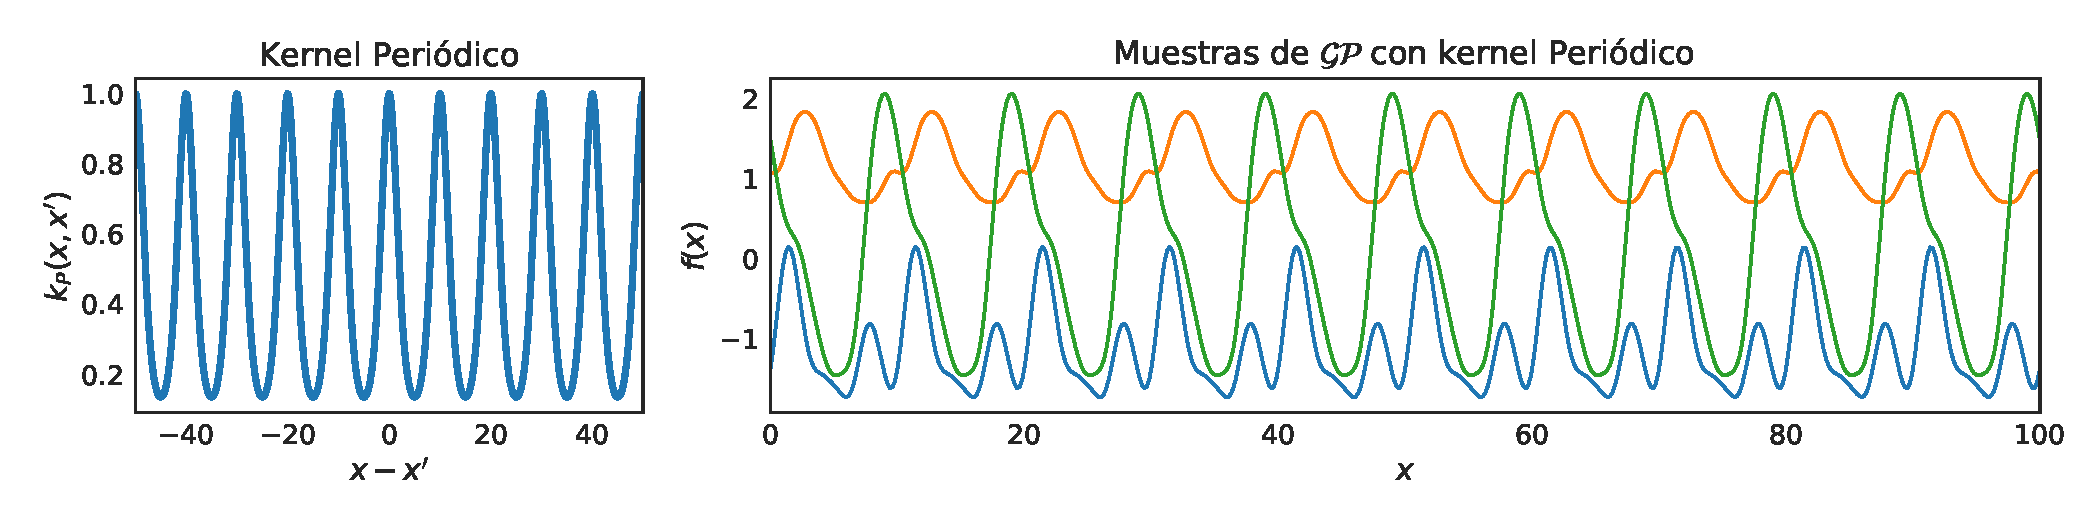
\includegraphics[width=0.9\textwidth]{img/gp_samples_P.pdf}
	\caption{Kernel periódico, en la izquierda se muestra la covarianza en función de su argumento $\tau=x-x'$, a la derecha de un $\gp$ usando un kernel periódico.}
	\label{fig:gp_7}
\end{figure}

\subsubsection{Operaciones con kernels}
A la hora de diseñar un $\gp$ y elegir una función de covarianza, no se está completamente limitado a kernels conocidos, sino que también se pueden combinar para obtener distintas funciones de covarianza y representar mejor el proceso.

Tanto la suma y multiplicación de kernels da como resultado un kernel válido que puede ser utilizado, también la exponencial de un kernel es también es un kernel, es decir $\exp(k_1(\cdot, \cdot))$ con $k_1$ un kernel válido.

\subsubsection{Representación espectral}
Un teorema importante para las funciones de covarianza en procesos débilmente estaicionarios es el teorema de Wiener–Khinchin, el cual dice que si para un proceso débilmente estacionario existe una función de covarianza $k(\tau)$ finita y definida para cualquier $\tau=x-x'$, entonces existe una función $S(\xi)$ tal que:

\begin{equation}\label{eq:gp_spectral}
	k(\tau) = \int S(\xi)e^{2\pi i \xi \cdot \tau} d\xi, \quad S(\xi)=\int k(\tau)e^{-2\pi i \xi \cdot \tau} d\tau
\end{equation}

Donde $i$ es la unidad imaginaria. $S(\xi)$ es conocida como la densidad espectral de potencia (PSD), en otras palabras, la función de covarianza $k(\tau)$ y la PSD $S(\xi)$ son duales de Fourier el uno del otro. Esto es extremadamente útil a la hora de diseñar funciones de covarianza pues este puede ser llevado a cavo en el dominio de la frecuencia y luego llevado a una función de covarianza usando la transformada inversa de Fourier.

\subsection{Extensiones para un $\gp$}
A continuación veremos un número de extensiones que se le pueden hacer a un $\gp$ para abordar distintos tipos de problemas.

\subsubsection{$\gp$ de clasificación}

\begin{wrapfigure}{r}{0.38\textwidth}
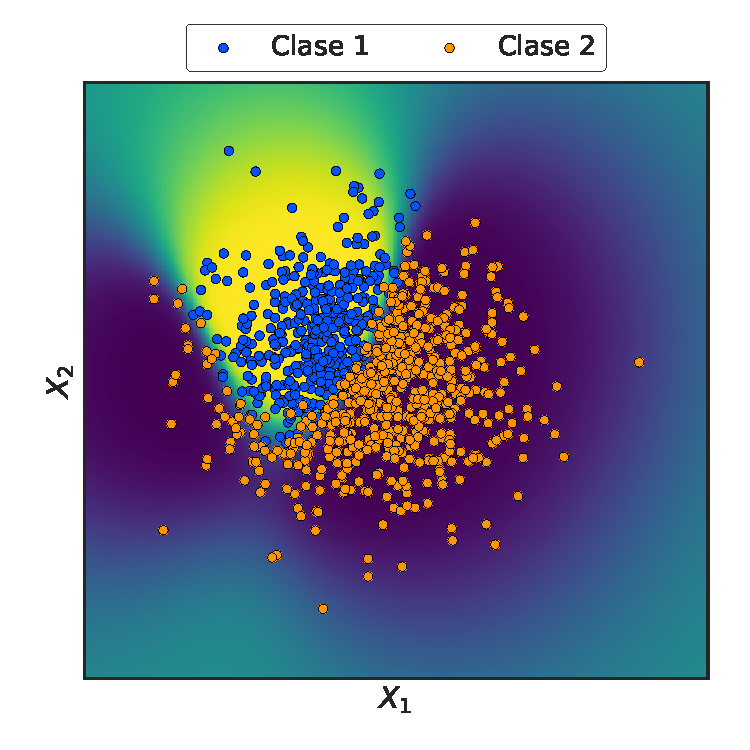
\includegraphics[width=0.38\textwidth]{img/gp_classifi.pdf}
\caption{$\gp$ de clasificación utilizando datos sintéticos. Este clasificador entrega una densidad de probabilidad en vez de una sola función de decisión.}\label{fig:gp_8}
\end{wrapfigure} 

Hasta el momento hemos visto como usar un $\gp$ para regresión, pero este también puede usado para clasificación, para esto simplemente ``pasamos'' nuestro $\gp$ por una función logística, para así obtener un prior sobre $\sigma\left(f(x)\right)$ donde $\sigma$ es la función logística. Sin embargo esto trae consigo un problema, pues ahora la distribución posterior a las observaciones no se tiene de forma analítica como para el caso de regresión, esto lleva a que tengamos que recurrir a métodos aproximado de inferencia. Una solución simple es utilizar la aproximación de Laplace, pero si se quieren aproximaciones más fidedignas métodos más complejos pueden ser usados como \textit{Expectation Maximization} y métodos MCMC. En la Fig.\ref{fig:gp_8} se muestra un ejemplo con datos sintéticos, a diferencia de la mayoría de los clasificadores vistos, este entrega naturalmente una densidad de probabilidad para la función de decisión.\\



\subsubsection{Selección automática de relevancia (ARD) (\textit{Selección automática de features})}
Un $\gp$ define una densidad de probabilidad sobre funciones, donde estas funciones son del tipo $f: \mathbb{R}^D \rightarrow \mathbb{R}$, con $D$ es finito, este es nuestra dimensión de entrada o ``características''. Haciendo un pequeño cambio en nuestra función kernel podemos hacer que esta automáticamente seleccione las entradas más relevantes con el problema, es decir realice una selección de características automática.\\

Si tomamos el kernel de la Ec.(\ref{eq:gp_ard}) vemos que es una multiplicación de kernels SE, donde se tiene un \textit{lenghtscale} por cada entrada $\ell_d$, sabemos que mientras más grande es este $\ell_d$ menos flexible será el $\gp$ respecto a cambios en ese eje, haciendo que las funciones del proceso dependan cada vez menos de la componente $d$ a medida que $\ell_d \rightarrow \infty$. De esta forma se puede controlar de forma automática la relevancia de cada eje del conjunto de entrada, pues los parámetros del kernel se obtienen en el entrenamiento. De esta forma estamos optimizando también en que grado afecta cada variable en nuestra predicción.

\begin{equation}\label{eq:gp_ard}
	k(x, x') = \sigma^2 \exp\left( -\sum_{d=1}^{D} \frac{(x_d - x_d')^2}{2\ell_d^2}\right)
\end{equation}


\subsubsection{Multi output $\gp$}
Hasta el momento solo hemos hablado de $\gp$ cuando nuestro proceso es solo una dimensión de salida. Se pueden extender los procesos Gaussianos a funciones de más de una salida o canal, donde ahora la función de covarianza $k(x, x')$ no entrega un escalar sino una matriz definida positiva, donde la diagonal corresponde a la covarianza del canal o autocovarianza y los elementos fuera de la diagonal corresponden a las covarianzas cruzadas o cross-covarianza. Este tipo de procesos Gaussianos aumentan considerablemente de complejidad al diseñar funciones de covarianza.\\ 

Dado un número $m$ de canales, se tendrán $m$ funciones de autocovarianza y ahora $m(m-1)/2$ funciones de covarianza y $k(x, x')$ será una matriz de $m\times m$. El desafio está en diseñar o escoger estas funciones de tal forma que para cualquier par de puntos $x$, $x'$ la matriz $k(x, x')$ sea definida positiva.

Una opción simple es asumir que los canales son independientes entre sí, lo que equivale a entrenar independientemente $m$ procesos Gaussianos, uno para cada canal, esto facilita el diseño de las funciones de covarianza pero hace que se pierdan relaciones entre los canales.
 

\subsection{Diferentes Interpretaciones de un $\gp$}

\subsubsection{De regresión lineal a $\gp$}

Partiendo de la regresión lineal donde el modelo es:

\begin{equation}
	y_i = w X_i + \epsilon_i
\end{equation}

Donde $\epsilon_i \sim \mathcal{N}(0, \sigma_n^2)$, luego podíamos extender este modelo usando $M$ funciones base $\phi_m$ y obtener:

\begin{equation}
	y_i = \sum_{m=1}^{M} w_m \phi(x_i) + \epsilon_i
\end{equation}

El paso siguiente es la regresión Bayesiana en base de funciones, donde agregamos un prior sobre los pesos $w_m \sim \mathcal{N}(0, \lambda_m^2)$, donde si obtenemos la covarianza de este proceso y marginalizamos por los pesos $w_m$ obtenemos:

\begin{equation}
	Cov(x, x') = k(x, x') = \sum_{m=1}^{M} \lambda_m^2 \phi_m(x)^T\phi_m(x') + \delta_{x, x'} \sigma_n^2
\end{equation}

Donde $\delta_{x, x'}$ el delta de Kronecker. Si nos damos cuenta esto define un $\gp$ con la función covarianza con un número finito de funciones bases. En general los $\gp$ corresponderán a covarianzas con infinitas funciones bases, como veremos a continuación.\\

Tomando un modelo sin ruido, con un número $M$ de funciones base $\phi_m$, donde sobre los pesos se define un prior i.i.d $w_m \sim \mathcal{N}(0, \sigma^2)$, tenemos:

\begin{equation}
	f(x) =  \sum_{m=1}^{M} w_m \phi(x)
\end{equation}
Y tomando $\phi=\exp(-\frac{1}{2\ell^2}(x- c_i)^2)$ donde $c_i$ son los centros de estas bases, y luego haciendo tender el número de funciones base $M$ a infinito tenemos que la covarianza es:

\begin{align}
	\mathbb{E}\left\{f(x) f(x')\right\} & = \sigma^2\sum_{m=1}^{M}  \phi_m(x)\phi_m(x') && \text{tomando } M\rightarrow \infty\\
	\mathbb{E}\left\{f(x) f(x')\right\} & \rightarrow \sigma^2 \int e^{-\frac{1}{2\ell^2}(x- c)^2} e^{-\frac{1}{2\ell^2}(x'- c)^2} dc \\
	& = \sigma^2 \sqrt{\pi\ell^2} e^{-\frac{1}{4\ell^2}(x- x')^2}\\
	& = k_{SE}(x, x')
\end{align}

Donde vemos que efectivamente el kernel SE es una función de covarianza para una composición infinita de funciones base.

\subsubsection{Nota sobre RKHS}
Dado un conjunto de entrenamiento $(X, Y) = \{x_i, y_i \}_{i=1}^{n}$ condicionando el proceso solo a una muestra de test $X_*=x_*$ y asumiendo una función media nula, de la Ec.(\ref{eq:gp_post}) para un $\gp$ la posterior de la media está dada por:

\begin{equation}
	\bar{f}(x_*) = m_{x_*|X} = k(X, x_*) (k(X, X) + \sigma_n \eye)^{-1} Y
\end{equation}

Y tomamos el vector $\bm{\alpha} = \left(k(X, X) + \sigma_n \eye \right)^{-1} Y$ obtenemos la expresión:

\begin{equation}
	\bar{f}(x_*) = \sum_{i=1}^{n} \alpha_i k(x_i, x_*)
\end{equation}

Donde, a pesar de que el proceso esta descrito por (posiblemente infinita) funciones base, aún así es la suma de finitos términos, cada uno centrado en un punto de entrenamiento, esto es debido al teorema del representante de los Espacios de Hilbert de Kernel Reproductor (RKHS). La intuición detrás de esto es que incluso si el $\gp$ induce una distribución conjunta sobre todos los $y = f(x)$, una para cada $x$ en el dominio, al hacer predicciones en el punto $x_*$ solo nos interesa la distribución $(n+1)$-dimensional definida por los puntos de entrenamiento más este punto de test.



\doublebox{
\begin{minipage}{\linewidth}
\centerline{\textbf{\underline{Resumen}}}

\textbf{¿Que es un Proceso Gaussiano?}\\
Un Proceso Gaussiano ($\gp$) es un método no paramétrico que define un \textit{prior sobre funciones}, lo cual se traduce en una \textit{posterior} sobre funciones si la verosimilitud es Gaussiana. Este proceso se encuentra caracterizado completamente por su función de media $m(\cdot)$ (generalmente se asume $0$) y función de covarianza o kernel $K_{\theta}(\cdot, \cdot)$ que puede depender o no de parámetros ($\theta$).\\

\textbf{¿Cómo se entrena?}\\
Dado un conjunto de entrenamiento $(\bx, \by)= \{(x_i, y_i)\}_{i=1}^{n}$, donde $y_i$ pueden estar contaminadas o no por ruido (generalmente se asume ruido Gaussiano de varianza $\sigma_n^2$)
se \textit{minimiza} la log-verosimilitud marginal negativa (NLL), que para el caso de $m(\cdot)=0$ es:

\begin{align}
	NLL & = -\log \pr(\by|\bx, \theta, \sigma_n) \\
	NLL & = \textcolor{blue}{\underbrace{ \color{black}{\frac{1}{2}\log|\mathbf{K_y}|} }_
	    {\text{\parbox{2cm}{\centering Penalización\\[-4pt] por\\[-4pt] complejidad}}}}
	    + \textcolor{Green}{\underbrace{ \color{black}{\frac{1}{2}\by^T \mathbf{K}_y^{-1} \by }}_
	    {\text{\parbox{2cm}{\centering Data fit }}}}
	    + \textcolor{red}{\underbrace{ \color{black}{\frac{n}{2} \log2\pi}}_
	    {\text{\parbox{2cm}{\centering Constante de normalización}}}} \label{eq:gp_nll_summary}
\end{align}

Donde $\mathbf{K}_y=K_{\theta}(\bx,\bx) + \sigma_n^2 \eye$.\\

\textbf{¿Cómo se evalúa en nuevos puntos?}\\
Si queremos evaluar en el conjunto de test $\rx$, la evaluación es:

\begin{align}
	& f(\rx)|\by, \bx  \sim \mathcal{N}(0, \Sigma_{\rx|\bx})\\ \label{eq:gp_posterior_summary}
	& \quad \text{Donde la media y covarianza son:} \nonumber \\
	m_{\rx|\bx} & = K(\rx, \bx) [K(\bx, \bx) + \sigma_n^2 \eye]^{-1} \by\\
	 \Sigma_{\rx|\bx} & = K(\rx, \rx) - K(\rx, \bx) [K(\bx, \bx) + \sigma_n^2 \eye]^{-1} K(\bx, \rx)
\end{align}

\textbf{¿Qué costo tiene?} 
\begin{itemize}
	\item Entrenamiento: $\mathcal{O}(n^3)$ respecto al número de muestras del conjunto de \textcolor{blue}{\textbf{entrenamiento}}.
	\item Evaluacion: $\mathcal{O}(n^2)$ respecto al número de muestras del conjunto de \textcolor{red}{\textbf{test}}.
\end{itemize}

\textbf{Notas sobre la implementación:}\\
Como la matriz de Gram ($K(X,X)$) es definida positiva y simétrica, para calcular su inversa de forma más eficiente se utiliza la descomposición de Cholesky, donde si $K=LL^T$, entonces $K^{-1}=(L^T)^{-1}L^{-1}$


\end{minipage}}\newpage
%!TEX root = ../notas_de_clase.tex

\section{Aprendizaje No Supervisado}

\subsection{Reducción de dimensionalidad}
\subsubsection{Análisis de componentes principales (ACP)}

Consideremos un conjunto de observaciones de $\{\x_i\}_{i=1}^n\subset\R^N$, donde denotamos $\x_i=[x_{i1},x_{i2},\ldots,x_{iN}]^\top$. Podemos entender que el elemento $x_{ij}$ corresponde al valor del atributo $j$ para la observación $i$. 

\begin{mdframed}[style=pendiente, frametitle={\center ejemplos}]
dar un ejemplo como el de nutrición, series de tiempo, geo-algo
\end{mdframed}

Notemos que cada observación puede descomponerse en la base canónica $\{\e_i\}_{i=1}^N$ de $\R^N$ de la forma 
\begin{equation}
	\x_i = x_{i1}\e_1 +  x_{i2}\e_2 + \cdots + x_{iN}\e_N 		
\end{equation}
Notemos que es posible representar cada vector $\x_i$ mediante una cantidad $N'<N$ de términos truncando la representación anterior, es decir,  
\begin{equation}
	\x_i \approx \sum_{j=1}^{N'} x_{i\sigma(j)}\e_{\sigma(j)}
\end{equation}
donde $\sigma:\{1,2,\ldots,N\}\mapsto\{1,2,\ldots,N\}$ es una permutación. Dicha aproximación de las observaciones $\{\x_i\}_{i=1}^n$ es una versión de baja dimensión, entonces, naturalmente nos podemos hacer la siguiente pregunta: dado una dimensión $N'<N$  ¿es efectivamente un subconjunto de los vectores canónicos la mejor base para descomponer as observaciones?  ¿cómo encontramos la \emph{mejor} base?

La respuesta a la primera pregunta es, en la mayoría de los casos, negativa. Esto es porque los elementos de la base canónica, por sí solos, conllevan poca información estructural que puede ser encontrada en los vectores observados. En particular, consideremos el caso en donde solo se dispone de dos observaciones $\{\x_1, \x_2\}$, si $N'=2$, entonces una descomposición que garantiza error nulo es simplemente elegir $\x_1$ y $\x_2$ como bases de la nueva descomposición, donde los coeficientes estarían dados por $[1,\ 0]^\top$ y $[0,\ 1]^\top$. 

Para encontrar la \emph{mejor} base, lo primero que se requiere es definir qué se entiende por \emph{mejor}. Nos enfocaremos en determinar una base cuyos componentes \textbf{ordenados} $\cvector_1,\cvector_2,\ldots$ capturan las $N'$ direcciones (ortogonales) de máxima variabilidad de nuestros datos. Es decir, el primer elemento de la nueva base estará dado por 
\begin{equation}
	\cvector_1 = \argmax_{||\cvector_1||=1} {\langle\cvector_1,\x\rangle} \label{eq:PCA_max}
\end{equation}
Este criterio es conocido como \textbf{análisis de componentes principales (ACP)}. Notemos que la restricción $||\cvector_1||=1$ es porque recordemos que estamos la dirección de máxima varianza y  la expresión anterior (cuadrática en $\cvector_1$) no es maximizable en $\cvector_1$. Por esta razón, sin pérdida de generalidad podemos fijar la norma de $\cvector_1$ en 1 y buscar una base \emph{ortonormal}. 

Asumiremos además que nuestros datos están estandarizados, es decir, tienen un vector de medias nulo y varianzas marginales unitarias. Esto es para reducir los sesgos por variables que pueden ser introducidos en la maximización de la expresión anterior: Si una dimensión tiene una varianza marginal mayor que el resto, ésta será más importante en la determinación de la dirección de máxima varianza solo por su magnitud y no por la relación entre variables. 

Como en general no contamos con la distribución de las observaciones $p(\x)$, podemos considerar una aproximación muestral de la varianza en la ecuación \eqref{eq:PCA_max} y resolver 
\begin{align}
	\cvector_1 = \argmax_{||\cvector_1||=1} \sum_{i=1}^N \langle\cvector_1,\x\rangle^2.\label{eq:PCA_max2}
\end{align}

Podemos ahora usar la siguiente notación
$$
X=[\x_1,\x_2,\ldots,,\x_n]=\begin{bmatrix}
        {x}_{11}    & \dots & {x}_{n1}  \\
        \cdots          & \ddots& \cdots        \\
        {x}_{1N}    & \dots & {x}_{nN}
        \end{bmatrix},
$$
y reescribir la ecuación \eqref{eq:PCA_max2} como 
\begin{align}
	\cvector_1 = \argmax_{||\cvector_1||=1} ||\cvector_1^\top X||^2 
			= \argmax_{||\cvector_1||=1} \cvector_1^\top XX^\top \cvector_1
			= \argmax_{\cvector_1} \frac{\cvector_1^\top XX^\top \cvector_1}{\cvector_1^\top \cvector_1}. 
			\label{eq:PCA_max3}
\end{align}
donde la última igualdad incorpora la normalización de $\cvector_1$ la cual permite formular el problema de optimización irrestricto. La expresión de la derecha se llama cuociente de Rayleigh para la matriz simétrica $XX^\top$, donde sabemos que la maximización de este cuociente está dado por el vector propio de la matriz $XX^\top$ asociado al mayor valor propio. Observe que $XX^\top$ es la matriz de correlación muestreal del conjunto de observaciones $\{\x_i\}_{i=1}^n$, consecuentemente, la proyección de una observación $\x_i$ en la dirección de máxima varianza, o bien la \emph{primera componente principal}, está dada por 
\begin{equation}
	\x_i^{(1)} = \langle \x_i, \cvector_1 \rangle
\end{equation}
donde $\cvector_1$ es el vector propio asociado al mayor valor propio de la matriz de covarianza muestreal $XX^\top$.

El cálculo de las siguientes componentes se realiza de forma iterativa sobre los residuos del conjunto de observaciones con respecto a las componentes anteriores. De esta forma, ACP encuentra una nueva base ortonormal tal que las componentes maximicen la variabilidad donde en algunos casos se puede perder intepretabilidad de las nuevas características generadas, pues son combinaciones lineales de las características originales de los datos. A pesar de esto, utilizando las primeras 2 o 3 componentes PCA se pueden visualizar datos de alta dimensionabilidad de forma ilustrativa.


\subsubsection{Kernel PCA}
El método Kernel PCA es similar a PCA, pero esta vez se utiliza el truco del kernel para proyectar los datos. En ese sentido, en vez de calcular la matriz de covarianza empírica, se utiliza la matriz de Gram.

$$
K_{ij} = K(x_i,x_j) = \phi(x_i)\phi(x_j)^T
$$

Luego, se prosigue de la misma forma que PCA linear.

En la figura \ref{fig:kpca} se puede observar un ejemplo en que el resultado de PCA linear no es suficiente, puesto que el problema es simétrico, mientras que KPCA realiza una correcta separación de ambos clusters.

\begin{figure}[ht]
    \centering
    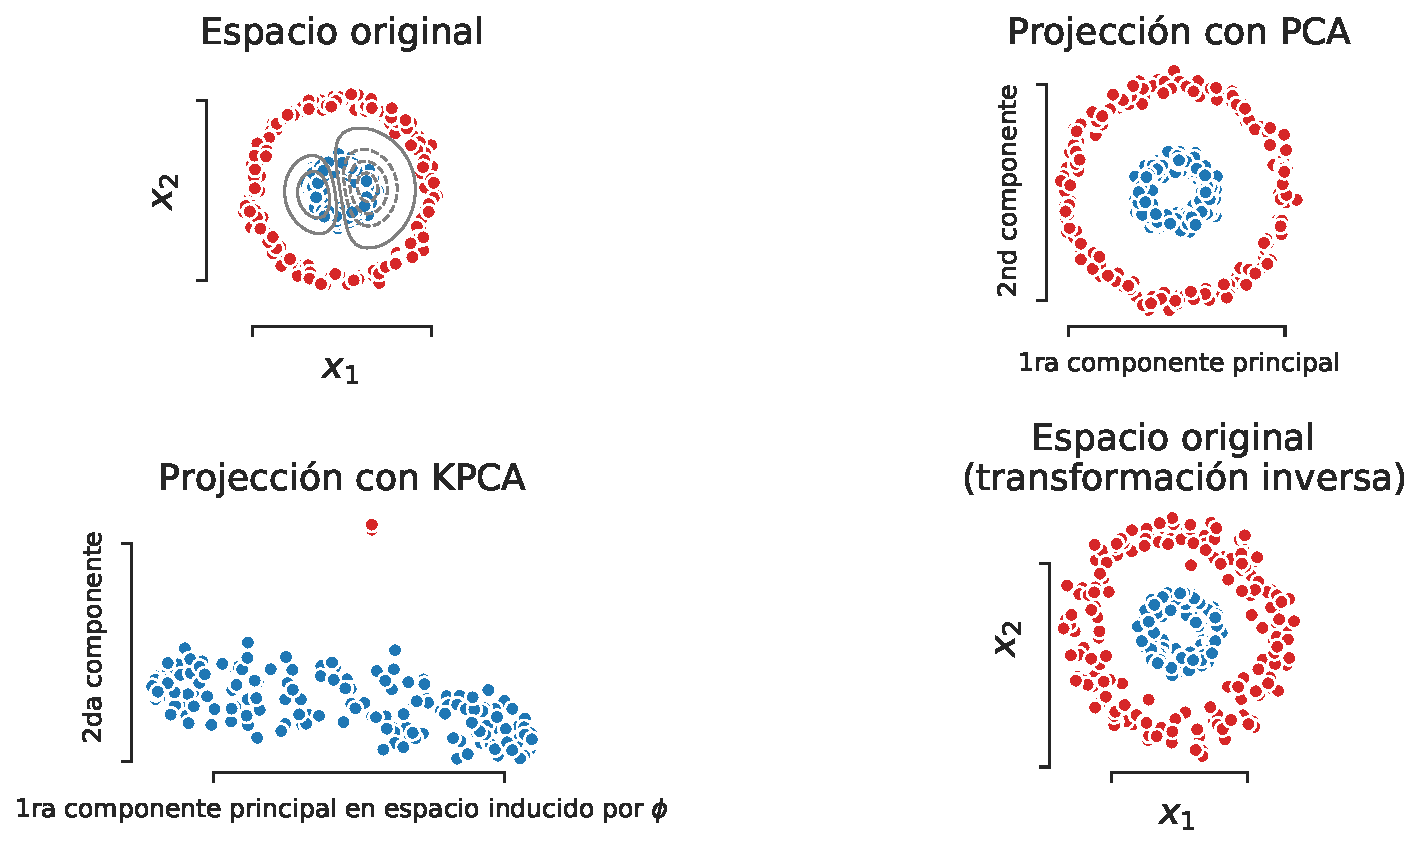
\includegraphics[width=0.7\linewidth]{img/cap7_kpca.pdf}
    \caption{Ejemplo en que kernel PCA sobre un conjunto de datos que no es linealmente separable.}
    \label{fig:kpca}
\end{figure}

\subsubsection{Probabilistic PCA}
PCA probabilístico (PPCA, por su sigla en inglés) tiene su inspiración en que PCA se puede expresar como la solución via máxima verosimilitud de un modelo probabilístico de variable latente. De este modo, PPCA propone un método iterativo para obtener la solución evaluando solo cierto número de componentes, sin necesidad de calcular la matriz de covarianza empírica.

El modelo probabilístico para PCA en que se inspira PPCA es el siguiente:

Sea $x_i\in \mathbb{R}^m$ los elementos observados, inputs o variables y $z\in \mathbb{R}^l$ una variable latente explícita correspondiente al espacio de las componentes principales. Se define un prior para $z$:

\begin{equation}
p(z) = N(0,I)
\end{equation}

De este modo, la distribución condicional de x dado z también es Gaussiana:

\begin{equation}
p(x|z) = N(Wz+\mu,\sigma^2I)
\end{equation}
Donde $W\in \mathbb{R}^{M\times l}$ y $\mu \in \mathbb{R}^m$ son parámetros a determinar. Notemos que no se pierde generalidad tomar el prior para $z$ con media cero y varianza unitaria, puesto que si se toma otro prior más general, se produce el mismo modelo.

Dado que tenemos modelo paramétrico probabilístico, podemos estimar los parámetros con máxima verosimilitud. Dado los datos $X = \{x_i\}_{i=1}^n$. La log-verosimilitud está dada por:

\begin{align}
\log p(X|W,\mu, \sigma^2) & = \sum_{i=1}^n \log p(x_i|W,\mu, \sigma^2)\\
& = \frac{n l}{2}\log (2\pi) - \frac{n}{2}log|C| - \frac{1}{2}\sum_{i=1}^n (x_i-\mu)^T C^{-1} (x_i-\mu),
\end{align}

con $C = WW^T + \sigma^2 I$.

Usando la condición de primer orden obtenemos

\begin{align}
\mu = \bar{x} = \frac{1}{n}\sum_{i=1}^n x_i.
\end{align}
De esta manera tenemos la función de log-verosimilitud completa:

\begin{align}
    \log p(X, Z|W, \mu, \sigma^2) = \sum_{i=1}^n \{\log p(x_i|z_i) + \log p(z_i)\}
\end{align}

y evaluando en $\mu = \bar{x}$

\begin{align}
\notag \mathbb{E}[ p(X,Z |W, \mu, \sigma^2) ] =  -\sum_{i=1}^n \Bigg\{ &\frac{l}{2} \log (2\pi \sigma^2)\\
\notag & + \frac{1}{2}\text{Tr}(\mathbb{E}[z_iz_i^T])\\
\notag & \frac{1}{2\sigma^2}||x_i - \mu||^2 - \frac{1}{\sigma^2}\mathbb{E}[z_i]^T W^T (x_i - \mu)\\
& \frac{1}{2\sigma^2} \text{Tr}(\mathbb{E}[z_iz_i^T]W^T W) \Bigg\}
\end{align}



\section{Clustering}

\subsection{k-means}
Dado un entero $k \in \mathbb{N}$ y uin conjunto de observaciones $X = \{x_i\}_{i=1}$ con $x_i\in \mathbb{R}^D$ queremos separar los datos en k graupos, donde cada grupo se le asigna un centroide $\mu_k$ y cada elemento $x_i$ se le asigna el grupo que tenga el centroide más cercano.

Sea $r_{ik}$ la asignación, esta estará definida por:

\begin{align*}
r_{ik} = \begin{cases}
1 & \text{si } k = \text{argmin}||x_i-x_k||\\
0 & \text{si no.}
\end{cases}
\end{align*}
Es decir, para encontrar los centroides se debe minimizar la función:

\begin{align}
J = \sum_{i=1}^N \sum_{k=1}^K r_{ik} ||x_i-x_j||^2
\end{align}

Para minimizar esta función utilizaremos un enfoque llamado \emph{Expectation-Maximization}. Este es un método iterativo y como tal, tiene problemas con mínimo locales, pero para solucionar esto, basta inicializar el algoritmo muchas veces.

El algoritmo está dado por:

\begin{itemize}
    \item \textbf{E-step:} En este paso, se calculan (actualizan) las asignaciones $r_{ik}$, dejando fijos $\mu_k$. Lo que corresponde a asignar el dato $x_i$ al centroide más cercano.
    \item \textbf{M-step:} El siguiente paso corresponde a actualizar los centroides $\mu_k$ dejando fijo las asignaciones $r_{ik}$.
    
    Como J es cuadrática en $\mu_k$, entonces podemos utilizar la condición de primer orden:
    \begin{align}
        \mu_k = \frac{\sum_{i=1}^N r_{ik}x_i}{\sum_{i=1}^N r_{ik}}
    \end{align}
    
    Lo que corresponde a asignar el centro del cluster al promedio de todas las muestras asignadas al antiguo cluster.
\end{itemize}

\underline{\textbf{Ejemplo:}} En la figura \ref{fig:kmeans} se observa un ejemplo de clustering utilizando kmeans. Como se puede notar, los clusters creados por kmeans son circulares, puesto que se utiliza distancia euclediana hace el centro del cluster.

\begin{figure}[ht]
  \centering
  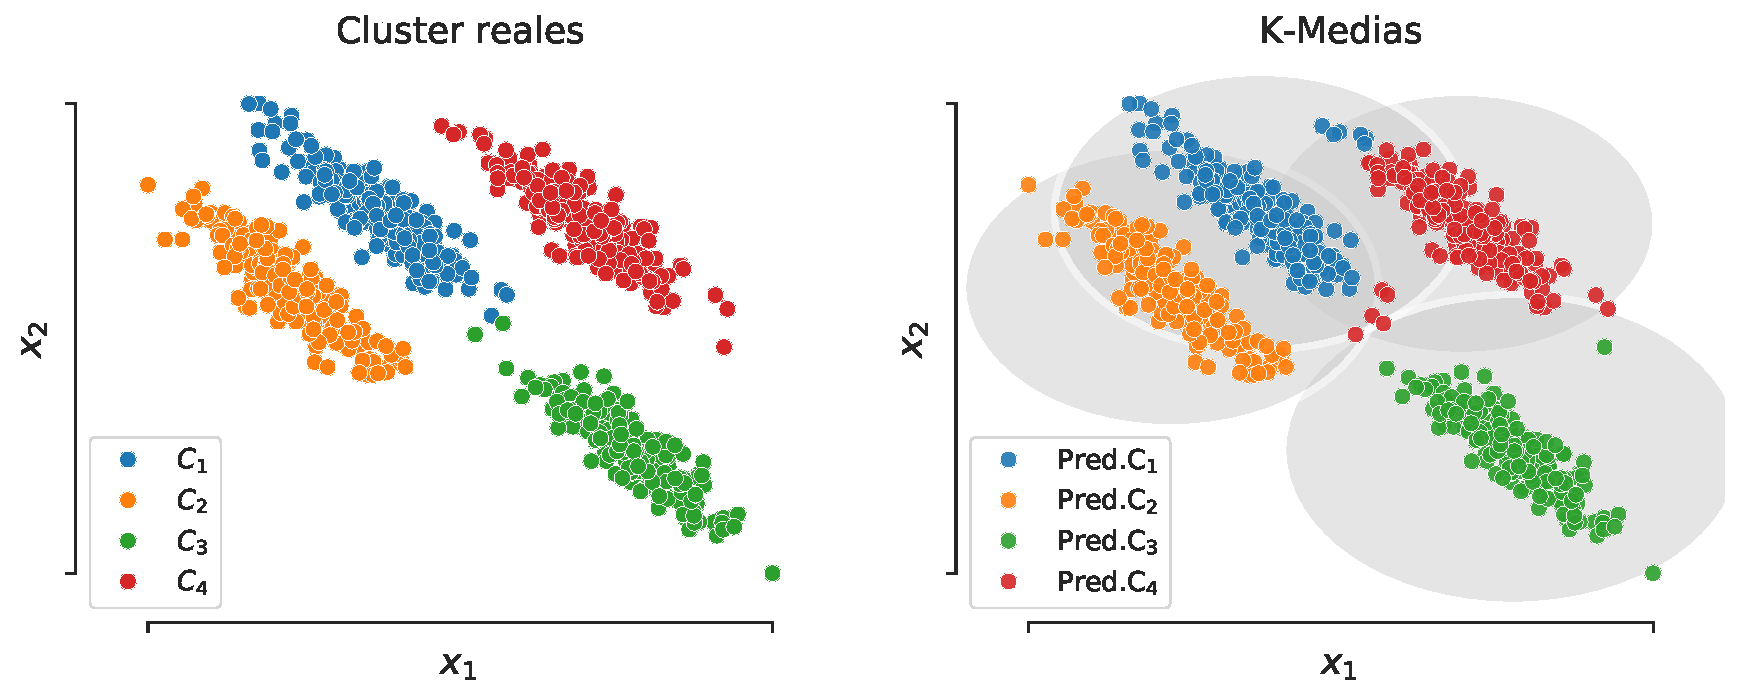
\includegraphics[width=0.8\textwidth]{img/cap7_k_medias}
  \caption{(Izquierda) Datos reales con sus etiquetas correctas. (Derecha) Clusters encontrados por k-means.}
  \label{fig:kmeans}
\end{figure}



\subsection{Modelo de mezcla de gaussianas}

La mezcla de gaussianas (GMM, por su sigla en inglés) es un caso general de k-means, en donde los clusters pueden tener una forma anisotrópica modelada por una Gaussiana con covarianza no necesariamente proporcional a la identidad. Además, si bien su solución puede ser muy similar a K-means los supuestos subyacentes al modelo CMM son diferentes y obedecen a un enfoque de modelo generativo. 

Recordemos que una distribución de mezcla de gaussianas dada por 
\begin{align}
p(\x) = \sum_{k=1}^K \pi_k \mathcal{N}(\xi| \mu_k,\Sigma_k)
\end{align}
es un modelo para aproximar distribuciones mediante la consideración de varias componentes $K\in\N$. Nos referiremos a los parámetros de este modelo como 

\begin{itemize}
	\item $\pi_k:$ coeficiente de mezcla del cluster  $k$
	\item $\mu_k:$ media del cluster  $k$
	\item $\Sigma_k:$ matriz de covarianza del cluster  $k$
\end{itemize}

En el caso de clustering, es necesario además saber de qué componente fue generada cada muestra. Con el mismo criterio que $K$-means, podemos asignar una variable latente, denotada $\z = [z_1,z_2,\ldots,z_K]^\top\in\{0,1\}^K$, que describe la asignación de cada muestra a cada cluster, es decir, $z_{k}=1$ si la observación $x_n$ pertenece al cluster $k$, y $z_{k}=0$ si no. 

Podemos denotar la distribución marginal del cluster $k$, es decir, de que una observación sea generada por la $k$-ésima componente como 
\begin{equation}
 	p(z_k=1) = \pi_k \label{eq:GMM_marg1}
\end{equation} 
con lo que la distribución marginal del vector $\z$ puede expresarse como 
\begin{equation}
	p(\z) = \prod_{k=1}^K \pi_k^{z_k} \label{eq:GMM_marg2}
\end{equation}
pues recordemos que $\sum_{k=1}^K {z_k} =1$ y $\sum_{k=1}^K {\pi_k}=1$. 

Adicionalmente, podemos describir la distribución condicional de $\x$, dado que su componente es la $k$-ésima, i.e., $z_k=1$, como 
\begin{equation}
	p(\x|z_{k}=1) = \cN(\x|\mu_k,\Sigma_k) \label{eq:GMM_cond1}
\end{equation}
y consecuente su distribución condicional como 
\begin{equation}
	p(\x|\z) = \left(\cN(\x|\mu_k,\Sigma_k)\right)^{z_k} \label{eq:GMM_cond2}
\end{equation}
Multiplicando las ecuaciones \eqref{eq:GMM_marg2} y \eqref{eq:GMM_cond2}, podemos obtener la distribución conjunta de $\x$ y $\z$, donde luego sumando  c.r.a. $k$, recuperamos la distribución marginal de $\x$ de suma de gaussianas mediante el uso de la variable latente $\z$. Respectivamente: 
\begin{align}
	p(\x,\z) &= \left(\pi_k\cN(\x|\mu_k,\Sigma_k)\right)^{z_k}\\
	p(\x) 	&= \sum_{k=1}^K p(\x,\z) = \sum_{k=1}^K \pi_k \cN(\x|\mu_k,\Sigma_k)
\end{align}

\begin{mdframed}[style=pendiente, frametitle={\center discusión}]
¿Por qué la conjunta es \emph{mejor} que la marginal?\\
Como generar muestras: ancestral sampling

\end{mdframed}


\subsubsection{Posterior} 
\label{sub:GMM_posterior}

Veamos ahora la forma que toma la distribución posterior de la variable latente $z$, usando el teorema de Bayes, tenemos 

\begin{align}
	p(z_k=1|\x) = \frac{p(\x|z_k=1)p(z_k=1)}{p(\x)} = \frac{\pi_k \cN(\x|\mu_k,\Sigma_k)}{\sum_{k=1}^K \pi_k \cN(\x|\mu_k,\Sigma_k)} \label{eq:GMM_post1}
\end{align}
esta cantidad también se llama \emph{responsabilidad} de la componente $k$ por la observación $\x$.

\subsubsection{Máxima verosimilitud} 
\label{sub:GMM_ml}

Recordemos que los parámetros del modelo de mezcla de gaussianas son los coeficientes de mezcla, las medias y varianzas de cada componente. Si disponemos de un conjunto de observaciones $\{\x_n\}_{n=1}^N$, entonces podemos encontrar dichos parámetros mediante máxima verosimilitud. Observe que la log-verosimilitud está dada por 

\begin{equation}
	\log p(\x_1,\x_2,\ldots,\x_N) = \sum_{n=1}^N \log p(\x_n) = \sum_{n=1}^N \log \sum_{k=1}^K  \pi_k\cN(\x_n|\mu_k,\Sigma_k) \label{eq:GMM_like}	
\end{equation}
Observemos que hay una serie de complicaciones relacionados a la búsqueda de estos parámetros mediante la maximización de las ecuación \eqref{eq:GMM_like}. Primero, están las soluciones dadas por singularidades cuando una muestra es exactamente igual a una de las medias, en cuyo caso un término de la log-verosimilitud es proporcional a $1/\sigma_k$, con lo que la maximización te $\sigma_k$ resulta en una log-verosimilitud infinita. En segundo lugar tenemos las redundancias de soluciones: para cada máximo local (o solución en general) de la log-verosimilitd existen $K!$ soluciones equivalente con la misma verosimilitud dadas por las permutaciones de las etiquetas de los clusters. Finalmente, optimizar la log-verosimilitud de la mezcla de gaussianas es desafiante porque la sumatoria aparece \emph{dentro} del logaritmo, consecuentemente,  el logaritmo no actúa directamente en la gaussiana reduciendo el funcional de optimización a una solución en forma cerrada. Por esta razón, es necesario considerar basados en gradiente.

\begin{mdframed}[style=pendiente, frametitle={\center discusión}]
¿Por qué no hay \emph{singularidades} en el caso de una gaussiana?
\end{mdframed}


\subsubsection{Entrenamiento} 
\label{sub:GMM_train}

Veamos las condiciones de primer orden para encontrar los parámetros, es decir, igualando el gradiente (con respecto a cada uno de los parámetros) de la log-verosimilitud igual a cero. Denotando $\gamma(z_{nk}) = p(z_{nk}=1|\x_n)$, obtenemos

 
    \begin{align}
    \mu_k & = \frac{1}{R_k}\sum_{n=1}^N \gamma(z_{nk})\x_i\\
    \Sigma_k & = \frac{1}{R_k} \sum_{n=1}^N \gamma(z_{nk})(\x_n - \mu_k)(\x_n - \mu_k)^\top\\
    \pi_k & = \frac{R_k}{R},
    \end{align}
    donde
    \begin{align*}
    R_k = \sum_{i=n}^N \gamma(z_{nk}) \qquad \text{y} \qquad R = \sum_{k=1}^K R_k.
    \end{align*}

  Observe que esto no constituye una solución en forma cerrada para los parámetros, pues la posterior $\gamma(z_{nk})$ depende de todos los parámetros de acuerdo a la ecuación \eqref{eq:GMM_post1}. Sin embargo, podemos considerar un procedimiento iterativo en donde calculamos las posteriores $\gamma(z_{nk})$ (llamado paso E), para luego calcular los parámetros óptimos de acuerdo a las ecuaciones anteriores (llamado paso M). 



\underline{\textbf{Ejemplo:}} La figura \ref{fig:gmm} muestra un ejemplo de clustering utilizando GMM. En este caso, se puede observar directamente como GMM es una generalización de kmeans, en donde ahora los clusters tienen forma de gaussiana anisotrópica.

\begin{figure}[ht]
  \centering
  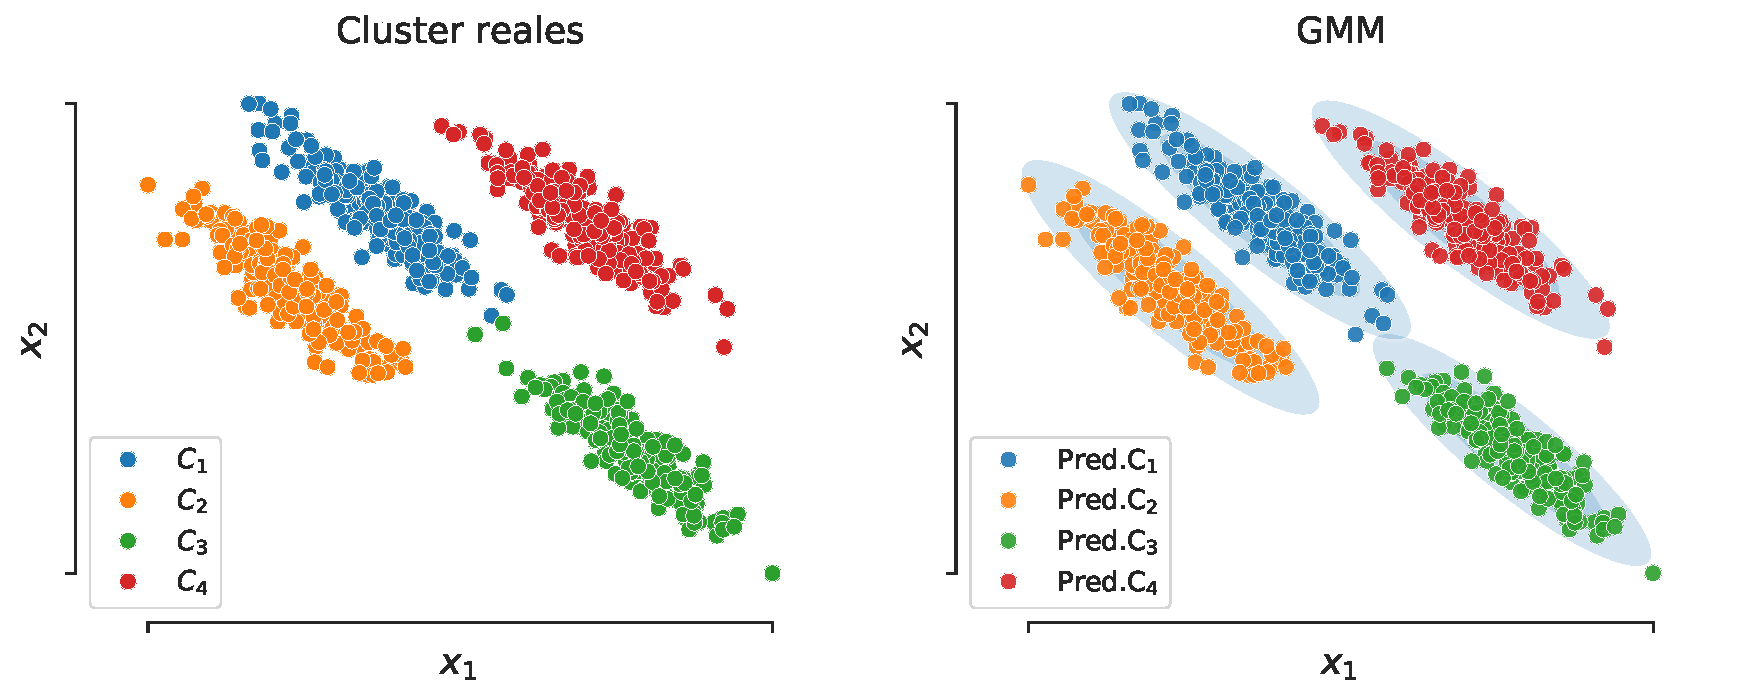
\includegraphics[width=0.8\textwidth]{img/cap7_gmm}
  \caption{(Izquierda) Datos reales con sus etiquetas correctas. (Derecha) Clusters encontrados por GMM.}
  \label{fig:gmm}
\end{figure}



\subsubsection{Expectation-Maximisation} 
\label{sub:GMM_EM}

En el caso general, donde tenemos \emph{observables} $\x$, variables latentes $\z$ y parámetros $\theta$, y un modelo descrito por una distribución marginal que puede ser expresada mediante 

\begin{equation}
	\log p(\x|\theta) = \log \int p(\x,\z|\theta)d\z
\end{equation}
donde tenemos logaritmos de sumas, lo cual es complicado de optimizar, incluso cuando la distribución conjunta $p(\x,\z|\theta)$ está en la familia exponencial.  

Asumamos por un momento que tenemos valores para la variable latente $\z$, si este fuese el caso, podríamos buscar los parámetros mediante la optimización de la log-verosimilitud completa, $\log p(\x, \z |\theta)$, la cual como en GMM puede tener una forma más simple de optimizar debido a que no hay una suma dentro del logaritmo. 

En la práctica, sin embargo, no tenemos acceso al valor de las variables latentes $\z_n$ sino que únicamente podemos acceder a una estimación de éstas mediante la distribución posterior $p(\z|\x,	\theta)$. Entonces, estrictamente hablado, la cantidad que nos gustaría maximizar $\log p(\x, \z |\theta)$ es aleatoria, por lo que podemos maximizar su esperanza con respecto a las observaciones (etapa de Maximización). Luego, con los valores obtenidos para los parámetros podemos recalcular la distribución posterior $p(\z|\x,\theta)$ (etapa de Esperanza) y seguir este proceso iterativamente. La motivación de este procedimiento, llamado \emph{Expectation-Maximisation}, es que en primer lugar, con la cantidad $p(\z|\x,\theta)$ fija, el cálculo de los nuevos parámetros mediante máxima verosimilitud indiscutiblemente aumenta la verosimilitud, luego éstos mejores parámetros dan consecuentemente una mejor estimación de la distribución posterior $p(\z|\x,\theta)$, con lo cual la actualización de los parámetros usando esta mejorada aproximación de la posterior debe ser incluso mejor. 

\begin{mdframed}[style=pendiente, frametitle={\center discusión}]
Bayesian GMM: ¿cómo elegir la cantidad de Gaussianas?
\end{mdframed}




\subsection{Density-based spatial clustering of applications with noise (DBSCAN)}

Es un algoritmo de clustering propuesto por Martin Ester et al. el cual ha tenido mucha popularidad puesto que no requiere definir una cantidad inicial de número de clusters. Los hiper-parámetros de entrada del modelo son 2:

\begin{itemize}
    \item Mínimo número de punto $minPts$.
    \item Radio o vecindad $\epsilon$.
\end{itemize}

El algoritmo se basa en la idea de que dado 2 púntos $x_i$, $x_j$ dentro de un mismo cluster, se dice que \emph{$x_i$ es alcanzable por $x_j$}, si siempre se puede llegar de $x_i$ a $x_j$ avanzando de punto en punto, donde la distancia entre cada uno es al menos menor que $\epsilon$ y además un punto intermedio es un punto núcleo. Con estos el algoritmo define tres tipos de puntos:

\begin{itemize}
    \item \textbf{Puntos núcleo:} Son puntos $x_i$ tales que en una vecindad $\epsilon$ tienen almenos $minPts$ vecinos.
    \item \textbf{Puntos borde:} Constituyen el \textit{borde externo} de los cluster.
    \item \textbf{Outliers:} Puntos que no son alcanzables por ningún punto.
\end{itemize}

Notemos que con lo anterior, se desprende que todo cluster debe tener al menos un punto núcleo.
El algoritmo para encontrar los clusters es el siguiente:


\begin{algorithm}[H]
  \caption{Pseudo código de DBSCAN
    \label{DBSCAN}}
  \begin{algorithmic}[1]
    \Function{DBSCAN}{$D, eps, MinPts$}
      \State $C \gets 0$\;
      \For{{cada punto $P$ no visitado en $D$}}
      \State marcar $P$ como visitado
        \If{sizeOf(PuntosVecinos) $\le$ MinPts}
        \State marcar $P$ como RUIDO
        \Else
        \State C $\gets$ C+1
        \State expandirCluster(P,vecinos, C, eps, MinPts)
        \EndIf
      \EndFor
    \EndFunction
  \end{algorithmic}
\end{algorithm}


\begin{algorithm}[H]
  \caption{Función para expandir cluster.
    \label{alg:expandirCluster}}
  \begin{algorithmic}[1]
  \Function{expandirCluster}{P, vecinosPts, C, eps, MinPts}
  \State agregar P al cluster C
  \For{cada punto P' en vecinosPts}
  \If{P' no fue visitado}
         \State marcar P' como visitado\;
         \State vecinosPts' $\gets$ regionDeConsulta(P', eps)\;
         \If{sizeof(vecinosPts') $\geq$ MinPts}
            \State vecinosPts $\gets$ vecinosPts $\cup$ vecinosPts'
        \EndIf
    \EndIf
    \If{P' no tiene cluster asignado}
         \State P' se le asigna el cluster C
    \EndIf
    \EndFor
    \EndFunction
  \end{algorithmic}
\end{algorithm}


\begin{algorithm}[H]
  \caption{Retorna los puntos de la vecindad de búsqueda para un punto.
    \label{alg:regionDeConsulta}}
  \begin{algorithmic}[1]
    \Function{regionDeConsulta}{$P, eps$}
    
    \Return Todos los puntos junto a P' que están a eps de distancia (incluyendo P)
    \EndFunction
  \end{algorithmic}
\end{algorithm}


\underline{\textbf{Ejemplo:}} La figura \ref{fig:dbscan} muestra un ejemplo de clustering utilizando DBSCAN. La figura \ref{fig:dbscan}(derecha) muestra en negro los puntos que son clasificados como ruido o \emph{outliers} por el algoritmo. Por otro lado, los puntos núcleos son graficados como un punto grande, mientras que los puntos borde se grafican con un marcador pequeño.

\begin{figure}[H]
  \centering
  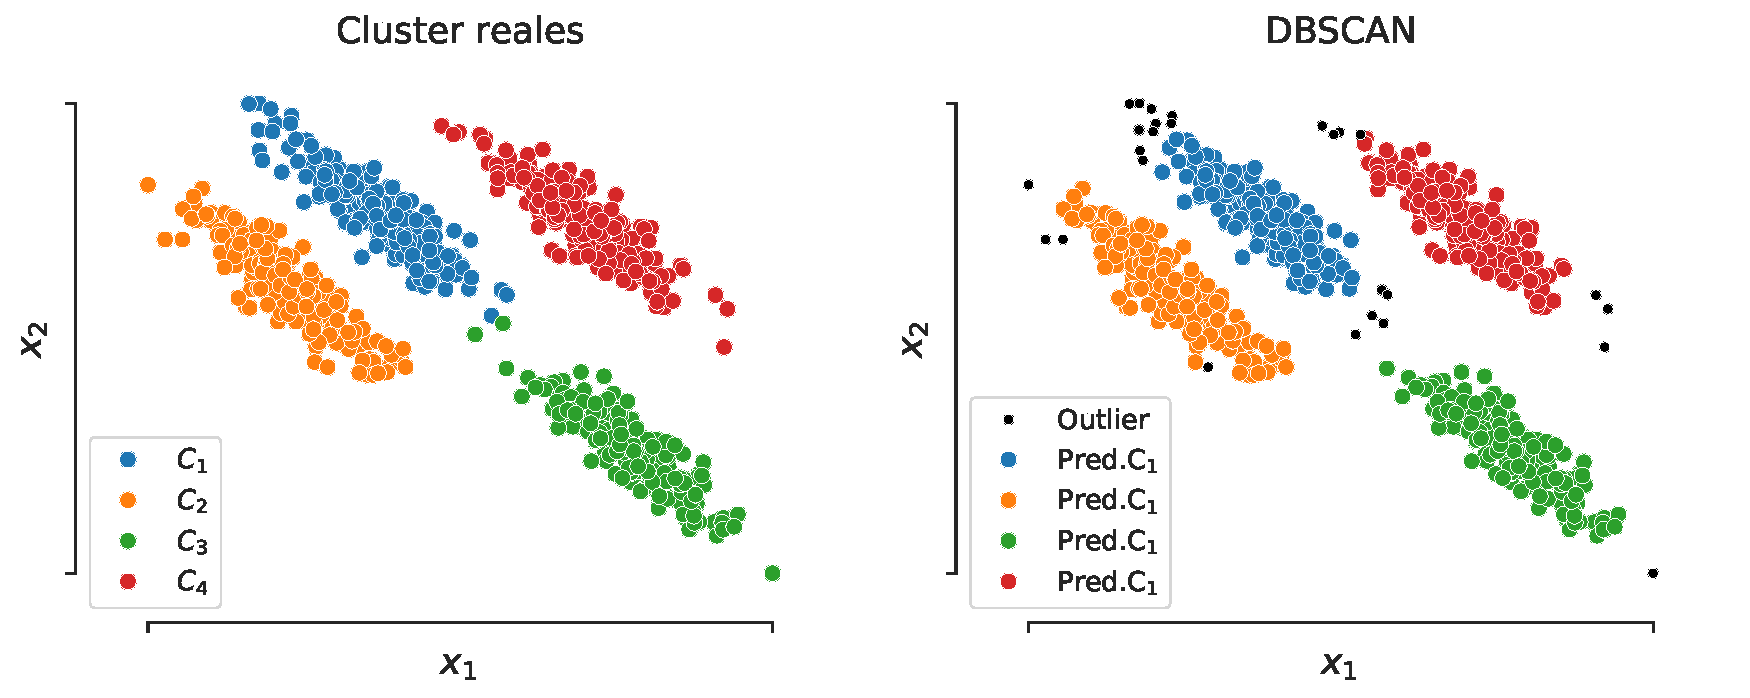
\includegraphics[width=0.8\textwidth]{img/cap7_dbscan}
  \caption{(Izquierda) Datos reales con sus etiquetas correctas. (Derecha) Clusters encontrados por DBSCAN.}
  \label{fig:dbscan}
\end{figure}\newpage
% subsection maximo_a_posteriori (end)
\bibliography{capitulos/referencias}
\bibliographystyle{apacite}


\end{document} 